%%%%%%%%%%%%%%%%%%%%%%%%%%%%%%%%%%%%%%%%%%%%%%%
%                                             %
% PERSONALIZACJa PRACY                        %
%                                             %
%%%%%%%%%%%%%%%%%%%%%%%%%%%%%%%%%%%%%%%%%%%%%%%

% dane autora
\newcommand{\FirstNameAuthor}{Szymon}
\newcommand{\SurnameAuthor}{Chmielewski}
\newcommand{\IdAuthor}{298498}   % numer albumu  (bez $\langle$ i $\rangle$)

% drugi autor:
%\newcommand{\FirstNameCoauthor}{Imię}   % Jeżeli jest drugi autor, to tutaj należy podać imię.
%\newcommand{\SurnameCoauthor}{Nazwisko} % Jeżeli jest drugi autor, to tutaj należy podać nazwisko.
%\newcommand{\IdCoauthor}{$\langle$wpisać właściwy$\rangle$}  % numer albumu drugiego autora (bez $\langle$ i $\rangle$)
% Gdy nie ma drugiego autora, należy zostawić poniższe definicje puste, jak poniżej. Gdy jest drugi autor, należy zakomentować te linie.
\newcommand{\FirstNameCoauthor}{} % Jeżeli praca ma tylko jednego autora, to dane drugiego autora zostają puste.
\newcommand{\SurnameCoauthor}{}   % Jeżeli praca ma tylko jednego autora, to dane drugiego autora zostają puste.
\newcommand{\IdCoauthor}{}  % Jeżeli praca ma tylko jednego autora, to dane drugiego autora zostają puste.
%%%%%%%%%%

\newcommand{\Supervisor}{Dr inż. Dominik Samociuk}     % dane promotora (bez $\langle$ i $\rangle$)
\newcommand{\Title}{Badanie wpływu zabezpieczeń w systemach IoT na prywatność i bezpieczeństwo użytkowników}           % tytuł pracy po polsku
\newcommand{\TitleAlt}{Study of the Impact of Security Measures in IoT Systems on User Privacy and Security}                     % thesis title in English
\newcommand{\Program}{Informatyka}            % kierunek studiów  (bez $\langle$ i $\rangle$)
\newcommand{\Specialisation}{Internet i technologie sieciowe}     % specjalność  (bez $\langle$ i $\rangle$)
\newcommand{\Departament}{Sieci i Systemów Komputerowych}        % katedra promotora  (bez $\langle$ i $\rangle$)
\newcommand{\Consultant}{} % brak promotowa pomocniczego / opiekuna



%%%%%%%%%%%%%%%%%%%%%%%%%%%%%%%%%%%%%%%%%%%%%%%
%                                             %
% PAKIETY, MAKRA, USTAWIENIA ITD.             %
%                                             %
%%%%%%%%%%%%%%%%%%%%%%%%%%%%%%%%%%%%%%%%%%%%%%%
\documentclass[a4paper,twoside,12pt]{book}
\usepackage[utf8]{inputenc}                                      
\usepackage[T1]{fontenc}  
\usepackage{amsmath,amsfonts,amssymb,amsthm}
\usepackage[british,polish]{babel} 
\usepackage{indentfirst}
\usepackage{xurl}
\usepackage{xstring}
\usepackage{ifthen}
\usepackage{hyperref}


\usepackage{ifxetex}

\ifxetex
	\usepackage{fontspec}
	\defaultfontfeatures{Mapping=tex—text} % to support TeX conventions like ``——-''
	\usepackage{xunicode} % Unicode support for LaTeX character names (accents, European chars, etc)
	\usepackage{xltxtra} % Extra customizations for XeLaTeX
\else
	\usepackage{lmodern}
\fi



\usepackage[margin=2.5cm]{geometry}
\usepackage{graphicx} 
\usepackage{hyperref}
\usepackage{booktabs}
\usepackage{tikz}
\usepackage{pgfplots}
\usepackage{mathtools}
\usepackage{geometry}
\usepackage{subcaption}   % subfigures
\usepackage[page]{appendix} % toc,
\renewcommand{\appendixtocname}{Dodatki}
\renewcommand{\appendixpagename}{Dodatki}
\renewcommand{\appendixname}{Dodatek}

\usepackage{csquotes}

\usepackage[backend=biber,style=ieee,maxbibnames=99]{biblatex}

%\usepackage[natbib=true,backend=bibtex,maxbibnames=99]{biblatex}  % kompilacja bibliografii BibTeXem
%\usepackage[natbib=true,backend=biber,maxbibnames=99]{biblatex}  % kompilacja bibliografii Biberem

%\bibliography{biblio/biblio}
\addbibresource{biblio/biblio.bib}

\usepackage{ifmtarg}   % empty commands  

\usepackage{setspace}
\onehalfspacing


\frenchspacing



%%%% TODO LIST GENERATOR %%%%%%%%%

\usepackage{color}
\definecolor{brickred}      {cmyk}{0   , 0.89, 0.94, 0.28}

\makeatletter \newcommand \kslistofremarks{\section*{Uwagi} \@starttoc{rks}}
  \newcommand\l@uwagas[2]
    {\par\noindent \textbf{#2:} %\parbox{10cm}
{#1}\par} \makeatother


\newcommand{\ksremark}[1]{%
{%\marginpar{\textdbend}
{\color{brickred}{[#1]}}}%
\addcontentsline{rks}{uwagas}{\protect{#1}}%
}

\newcommand{\comma}{\ksremark{przecinek}}
\newcommand{\nocomma}{\ksremark{bez przecinka}}
\newcommand{\styl}{\ksremark{styl}}
\newcommand{\ortografia}{\ksremark{ortografia}}
\newcommand{\fleksja}{\ksremark{fleksja}}
\newcommand{\pauza}{\ksremark{pauza `--', nie dywiz `-'}}
\newcommand{\kolokwializm}{\ksremark{kolokwializm}}
\newcommand{\cudzyslowy}{\ksremark{,,polskie cudzysłowy''}}

%%%%%%%%%%%%%% END OF TODO LIST GENERATOR %%%%%%%%%%%

\newcommand{\printCoauthor}{%		
    \StrLen{\FirstNameCoauthor}[\FNCoALen]
    \ifthenelse{\FNCoALen > 0}%
    {%
		{\large\bfseries\Coauthor\par}
	
		{\normalsize\bfseries \LeftId: \IdCoauthor\par}
    }%
    {}
} 

%%%%%%%%%%%%%%%%%%%%%
\newcommand{\autor}{%		
    \StrLen{\FirstNameCoauthor}[\FNCoALenXX]
    \ifthenelse{\FNCoALenXX > 0}%
    {\FirstNameAuthor\ \SurnameAuthor, \FirstNameCoauthor\ \SurnameCoauthor}%
	{\FirstNameAuthor\ \SurnameAuthor}%
}
%%%%%%%%%%%%%%%%%%%%%

\StrLen{\FirstNameCoauthor}[\FNCoALen]
\ifthenelse{\FNCoALen > 0}%
{%
\author{\FirstNameAuthor\ \SurnameAuthor, \FirstNameCoauthor\ \SurnameCoauthor}
}%
{%
\author{\FirstNameAuthor\ \SurnameAuthor}
}%

%%%%%%%%%%%% ZYWA PAGINA %%%%%%%%%%%%%%%
% brak kapitalizacji zywej paginy
\usepackage{fancyhdr}
\pagestyle{fancy}
\fancyhf{}
\fancyhead[LO]{\nouppercase{\it\rightmark}}
\fancyhead[RE]{\nouppercase{\it\leftmark}}
\fancyhead[LE,RO]{\it\thepage}


\fancypagestyle{tylkoNumeryStron}{%
   \fancyhf{} 
   \fancyhead[LE,RO]{\it\thepage}
}

\fancypagestyle{bezNumeracji}{%
   \fancyhf{} 
   \fancyhead[LE,RO]{}
}


\fancypagestyle{NumeryStronNazwyRozdzialow}{%
   \fancyhf{} 
   \fancyhead[LE]{\nouppercase{\autor}}
   \fancyhead[RO]{\nouppercase{\leftmark}} 
   \fancyfoot[CE, CO]{\thepage}
}


%%%%%%%%%%%%% OBCE WTRETY  
\newcommand{\obcy}[1]{\emph{#1}}
\newcommand{\english}[1]{{\selectlanguage{british}\obcy{#1}}}
%%%%%%%%%%%%%%%%%%%%%%%%%%%%%

% polskie oznaczenia funkcji matematycznych
\renewcommand{\tan}{\operatorname {tg}}
\renewcommand{\log}{\operatorname {lg}}

% jeszcze jakies drobiazgi

\newcounter{stronyPozaNumeracja}

%%%%%%%%%%%%%%%%%%%%%%%%%%% 
\newcommand{\printOpiekun}[1]{%		

    \StrLen{\Consultant}[\mystringlen]
    \ifthenelse{\mystringlen > 0}%
    {%
       {\large{\bfseries OPIEKUN, PROMOTOR POMOCNICZY}\par}
       
       {\large{\bfseries \Consultant}\par}
    }%
    {}
} 
%
%%%%%%%%%%%%%%%%%%%%%%%%%%%%%%%%%%%%%%%%%%%%%%
 
% Proszę nie modyfikować poniższych definicji!
\newcommand{\Author}{\FirstNameAuthor\ \MakeUppercase{\SurnameAuthor}} 
\newcommand{\Coauthor}{\FirstNameCoauthor\ \MakeUppercase{\SurnameCoauthor}}
\newcommand{\Type}{PRACA MAGISTERSKA}
\newcommand{\Faculty}{Wydział Automatyki, Elektroniki i Informatyki} 
\newcommand{\Polsl}{Politechnika Śląska}
\newcommand{\Logo}{graf/politechnika_sl_logo_bw_pion_pl.pdf}
\newcommand{\LeftId}{Nr albumu}
\newcommand{\LeftProgram}{Kierunek}
\newcommand{\LeftSpecialisation}{Specjalność}
\newcommand{\LeftSUPERVISOR}{PROWADZĄCY PRACĘ}
\newcommand{\LeftDEPARTMENT}{KATEDRA}
%%%%%%%%%%%%%%%%%%%%%%%%%%%%%%%%%%%%%%%%%%%%%%

%%%%%%%%%%%%%%%%%%%%%%%%%%%%%%%%%%%%%%%%%%%%%%%
%                                             %
% KONIEC USTAWIEŃ                             %
%                                             %
%%%%%%%%%%%%%%%%%%%%%%%%%%%%%%%%%%%%%%%%%%%%%%%

 

%%%%%%%%%%%%%%%%%%%%%%%%%%%%%%%%%%%%%%%%%%%%%%%
%                                             %
% MOJE PAKIETY, USTAWIENIA ITD                %
%                                             %
%%%%%%%%%%%%%%%%%%%%%%%%%%%%%%%%%%%%%%%%%%%%%%%

% Tutaj proszę umieszczać swoje pakiety, makra, ustawienia itd.


 
%%%%%%%%%%%%%%%%%%%%%%%%%%%%%%%%%%%%%%%%%%%%%%%%%%%%%%%%%%%%%%%%%%%%%
% listingi i fragmentu kodu źródłowego 
% pakiet: listings lub minted
% % % % % % % % % % % % % % % % % % % % % % % % % % % % % % % % % % % 

% biblioteka listings
\usepackage{listings}
\lstset{%
morekeywords={string,exception,std,vector},% słowa kluczowe rozpoznawane przez pakiet listings
language=C++,% C, Matlab, Python, SQL, TeX, XML, bash, ... – vide https://www.ctan.org/pkg/listings
commentstyle=\textit,%
identifierstyle=\textsf,%
keywordstyle=\sffamily\bfseries, %\texttt, %
%captionpos=b,%
tabsize=3,%
frame=lines,%
numbers=left,%
numberstyle=\tiny,%
numbersep=5pt,%
breaklines=true,%
escapeinside={@*}{*@},%
}

% % % % % % % % % % % % % % % % % % % % % % % % % % % % % % % % % % % 
% pakiet minted
%\usepackage{minted}

% pakiet wymaga specjalnego kompilowania:
% pdflatex -shell-escape main.tex
% xelatex  -shell-escape main.tex

%\usepackage[chapter]{minted} % [section]
%%\usemintedstyle{bw}   % czarno-białe kody 
%
%\setminted % https://ctan.org/pkg/minted
%{
%%fontsize=\normalsize,%\footnotesize,
%%captionpos=b,%
%tabsize=3,%
%frame=lines,%
%framesep=2mm,
%numbers=left,%
%numbersep=5pt,%
%breaklines=true,%
%escapeinside=@@,%
%}

%%%%%%%%%%%%%%%%%%%%%%%%%%%%%%%%%%%%%%%%%%%%%%%%%%%%%%%%%%%%%%%%%%%%%



%%%%%%%%%%%%%%%%%%%%%%%%%%%%%%%%%%%%%%%%%%%%%%%
%                                             %
% KONIEC MOICH USTAWIEŃ                       %
%                                             %
%%%%%%%%%%%%%%%%%%%%%%%%%%%%%%%%%%%%%%%%%%%%%%%

 
\usepackage{enumitem}
\usepackage{listings}
\usepackage{xcolor}
\usepackage{hyperref}
\usepackage{rotating} 
\usepackage{graphicx} 
\usepackage{array}    
\usepackage{booktabs} 
\usepackage{lipsum}   
\usepackage{pdflscape}

\lstset{
  language=Python,
  basicstyle=\ttfamily\small,
  keywordstyle=\color{blue},
  stringstyle=\color{orange},
  commentstyle=\color{gray},
  numbers=left,
  numberstyle=\tiny\color{gray},
  stepnumber=1,
  frame=single,
  breaklines=true,
  showstringspaces=false,
}

\begin{document}
%\kslistofremarks

\frontmatter

%%%%%%%%%%%%%%%%%%%%%%%%%%%%%%%%%%%%%%%%%%%%%%%
%                                             %
% PROSZĘ NIE MODYFIKOWAĆ STRONY TYTUŁOWEJ!    %
%                                             %
%%%%%%%%%%%%%%%%%%%%%%%%%%%%%%%%%%%%%%%%%%%%%%%


%%%%%%%%%%%%%%%%%%  STRONA TYTUŁOWA %%%%%%%%%%%%%%%%%%%
\pagestyle{empty}
{
	\newgeometry{top=1.5cm,%
	             bottom=2.5cm,%
	             left=3cm,
	             right=2.5cm}
 
	\ifxetex 
	  \begingroup
	  \setsansfont{Calibri}
	   
	\fi 
	 \sffamily
	\begin{center}
	\includegraphics[width=50mm]{\Logo}
	 
	
	{\Large\bfseries\Type\par}
	
	\vfill  \vfill  
			 
	{\large\Title\par}
	
	\vfill  
		
	{\large\bfseries\Author\par}
	
	{\normalsize\bfseries \LeftId: \IdAuthor}

	\printCoauthor
	
	\vfill  		
 
	{\large{\bfseries \LeftProgram:} \Program\par} 
	
	{\large{\bfseries \LeftSpecialisation:} \Specialisation\par} 
	 		
	\vfill  \vfill 	\vfill 	\vfill 	\vfill 	\vfill 	\vfill  
	 
	{\large{\bfseries \LeftSUPERVISOR}\par}
	
	{\large{\bfseries \Supervisor}\par}
				
	{\large{\bfseries \LeftDEPARTMENT\ \Departament} \par}
		
	{\large{\bfseries \Faculty}\par}
		
	\vfill  \vfill  

    	
    \printOpiekun{\Consultant}
    
	\vfill  \vfill  
		
    {\large\bfseries  Gliwice \the\year}

   \end{center}	
       \ifxetex 
       	  \endgroup
       \fi
	\restoregeometry
}
  
%%%%%%%%%%%%%%%%%%%%%%%%%%%%%%%%%%%%%%%%%%%%%%%
%                                             %
% KONIEC STRONY TYTUŁOWEJ                     %
%                                             %
%%%%%%%%%%%%%%%%%%%%%%%%%%%%%%%%%%%%%%%%%%%%%%%  




\lstset{
  language=Python,
  basicstyle=\ttfamily\small,
  keywordstyle=\color{blue},
  stringstyle=\color{orange},
  commentstyle=\color{gray},
  numbers=left,
  numberstyle=\tiny\color{gray},
  stepnumber=1,
  frame=single,
  breaklines=true,
  showstringspaces=false,
}


\cleardoublepage

\rmfamily\normalfont
\pagestyle{empty}

%%%%%%%%%%%%%%%%%%%%%%%%%%%%%%%%%%%%%%%%%%%%%%%
%                                             %
% CHAPTER 0                                   %
%                                             %
%%%%%%%%%%%%%%%%%%%%%%%%%%%%%%%%%%%%%%%%%%%%%%%

\subsubsection*{Tytuł pracy} 
\Title

\subsubsection*{Streszczenie}  
Praca magisterska poświęcona jest zagadnieniom bezpieczeństwa i ochrony prywatności w systemach Internetu Rzeczy (IoT). Wraz z dynamicznym rozwojem technologii IoT rośnie znaczenie skutecznych mechanizmów zabezpieczających, które muszą jednocześnie chronić dane użytkowników i uwzględniać ograniczenia zasobowe urządzeń.

W pracy przeanalizowano kluczowe wyzwania związane z bezpieczeństwem w IoT, w tym zagrożenia takie jak nieautoryzowany dostęp, ataki typu DDoS czy naruszenia prywatności. Omówiono stosowane obecnie rozwiązania techniczne, w tym metody szyfrowania, protokoły komunikacyjne i systemy uwierzytelniania, zwracając szczególną uwagę na ich wpływ na wydajność systemów IoT.

Głównym celem badania było znalezienie optymalnej równowagi między poziomem bezpieczeństwa, ochroną prywatności użytkowników a efektywnym wykorzystaniem zasobów urządzeń IoT. W pracy zaproponowano szereg rozwiązań optymalizacyjnych, które mogą przyczynić się do poprawy bezpieczeństwa systemów IoT bez nadmiernego obciążania ich ograniczonych możliwości obliczeniowych.

Wyniki przeprowadzonych analiz mogą stanowić wartościowy punkt wyjścia dla producentów urządzeń IoT oraz dostawców rozwiązań chmurowych, pomagając w projektowaniu bardziej bezpiecznych i przyjaznych dla użytkownika systemów Internetu Rzeczy. Praca wskazuje także kierunki dalszych badań w tej dynamicznie rozwijającej się dziedzinie.

\subsubsection*{Słowa kluczowe} 
Internet Rzeczy (IoT), bezpieczeństwo cybernetyczne, ochrona prywatności, szyfrowanie danych, optymalizacja zabezpieczeń
\newpage
\subsubsection*{Thesis title} 
\begin{otherlanguage}{british}
\TitleAlt
\end{otherlanguage}

\subsubsection*{Abstract} 
\begin{otherlanguage}{british}
This master's thesis focuses on security and privacy issues in Internet of Things (IoT) systems. As IoT technology rapidly develops, there is a growing need for effective security mechanisms that can protect user data while accounting for device resource limitations.

The study examines key IoT security challenges, including threats such as unauthorized access, DDoS attacks, and privacy breaches. It analyzes current technical solutions, including encryption methods, communication protocols, and authentication systems, with particular attention to their impact on IoT system performance.

The main research objective was to find an optimal balance between security levels, user privacy protection, and efficient utilization of IoT device resources. The thesis proposes several optimization approaches that could enhance IoT security without excessively straining the limited computational capabilities of these devices.

The analysis results provide valuable insights for IoT device manufacturers and cloud solution providers, supporting the development of more secure and user-friendly IoT systems. The study also identifies promising directions for future research in this rapidly evolving field.
\end{otherlanguage}
\subsubsection*{Key words}  
\begin{otherlanguage}{british}
Internet of Things (IoT), cybersecurity, privacy protection, data encryption, security optimization
\end{otherlanguage}

 % informacje redakcyjne

%%%%%%%%%%%%%%%%%% SPIS TRESCI %%%%%%%%%%%%%%%%%%%%%%
% Add \thispagestyle{empty} to the toc file (main.toc), because \pagestyle{empty} doesn't work if the TOC has multiple pages
\addtocontents{toc}{\protect\thispagestyle{empty}}
\tableofcontents

%%%%%%%%%%%%%%%%%%%%%%%%%%%%%%%%%%%%%%%%%%%%%%%%%%%%%
\setcounter{stronyPozaNumeracja}{\value{page}}
\mainmatter
\pagestyle{empty}

\cleardoublepage

\pagestyle{NumeryStronNazwyRozdzialow}

%%%%%%%%%%%%%%%%%%%%%%%%%%%%%%%%%%%%%%%%%%%%%%%
%                                             %
% TREŚĆ WŁAŚCIWA PRACY                        %
%                                             %
%%%%%%%%%%%%%%%%%%%%%%%%%%%%%%%%%%%%%%%%%%%%%%%

% TODO
\chapter{Wstęp}

\section{Cel i zakres pracy}
Głównym celem niniejszej pracy jest kompleksowa analiza wpływu współczesnych mechanizmów bezpieczeństwa na ochronę prywatności użytkowników w systemach Internetu Rzeczy (IoT) oraz opracowanie rekomendacji optymalizujących ich wdrożenie. Praca koncentruje się na zbadaniu, w jaki sposób stosowane rozwiązania techniczne, takie jak szyfrowanie danych czy systemy uwierzytelniania, oddziałują na poziom bezpieczeństwa i prywatności w środowisku IoT. W szczególności analizowane są kompromisy między skutecznością ochrony danych a wydajnością systemów oraz zasobami ograniczonych urządzeń IoT.
Przedmiotem analizy są zarówno teoretyczne aspekty bezpieczeństwa, jak i praktyczne testy w kontrolowanym środowisku, mające na celu weryfikację rzeczywistej skuteczności zabezpieczeń.
Finalnym celem pracy jest opracowanie praktycznych rekomendacji optymalizujących bezpieczeństwo systemów IoT bez nadmiernego pogarszania ich funkcjonalności i wydajności. Dodatkowym celem jest podniesienie świadomości użytkowników oraz osób bezpośrednio zaangażowanych w pracę lub rozwój takich urządzeń, aby zwiększyć ich zdolność do identyfikacji zagrożeń i skutecznego wdrażania środków ochrony.
\subsection{Hipotezy badawcze}
W oparciu o cele pracy, sformułowano następujące hipotezy badawcze:

\begin{enumerate}[]
    \item \textbf{Hipoteza H1} - Stosowanie standardowych mechanizmów bezpieczeństwa (szyfrowanie danych, uwierzytelnianie, autoryzacja) znacząco zmniejsza ryzyko naruszenia prywatności użytkowników w systemach IoT.
    \item \textbf{Hipoteza H2} - Niskokosztowe środki ochrony, jeśli są prawidłowo wdrożone, wykazują wysoką skuteczność przy minimalnym wpływie na wydajność urządzeń.
    \item \textbf{Hipoteza H3} - Wiele popularnych urządzeń IoT nie spełnia wymogów regulacyjnych dotyczących ochrony danych, co zwiększa ryzyko prawne dla użytkowników i organizacji.
    \item \textbf{Hipoteza H4} - Optymalizacja algorytmów bezpieczeństwa może znacząco poprawić równowagę między bezpieczeństwem, prywatnością a wydajnością systemów IoT.
\end{enumerate}

\section{Motywacja do podjęcia tematu}
Dynamiczny rozwój Internetu Rzeczy (IoT), którego globalna skala według najnowszych danych osiągnęła już ponad 18 miliardów podłączonych urządzeń \cite{iotanalytics2024}, stanowi główną przesłankę do podjęcia niniejszych badań. Obszerne spektrum zastosowań IoT — od inteligentnych domów i urządzeń noszonych po infrastrukturę przemysłową (IIoT) — wskazuje na pilną potrzebę systemowej analizy efektywności współczesnych mechanizmów bezpieczeństwa. Istotnym aspektem problemu badawczego jest fundamentalny paradoks współczesnego IoT: z jednej strony potencjał usprawniający różne aspekty ludzkiego życia, z drugiej zaś — rosnące zagrożenia dla prywatności i bezpieczeństwa danych.

Analiza głośnych przypadków naruszeń bezpieczeństwa, takich jak incydent z kamerami \hyperref[subsec:mirai]{Mirai} w 2021 roku, który dotknął ponad 500 000 użytkowników \cite{sharad2020mirai}, ujawnia systemowe słabości obecnych rozwiązań. Jednocześnie badania rynkowe wskazują, że wielu producentów urządzeń IoT priorytetowo traktuje funkcjonalność, marginalizując kwestie ochrony prywatności, co znajduje odzwierciedlenie w decyzjach konsumentów \cite{cisco2024}. Właśnie owo napięcie między innowacyjnością a bezpieczeństwem stało się kluczową przesłanką do podjęcia przedstawionych badań. 

\section{Struktura pracy}
Niniejsza praca ma na celu kompleksową analizę zagadnień związanych z bezpieczeństwem i prywatnością w systemach Internetu Rzeczy (IoT), ze szczególnym uwzględnieniem oceny istniejących mechanizmów zabezpieczających, ich testowania w kontrolowanym środowisku oraz propozycji optymalizacji. Struktura pracy została zaprojektowana tak, aby w logiczny sposób poprowadzić czytelnika od wprowadzenia teoretycznego, przez badania praktyczne, aż do sformułowania wniosków i rekomendacji.

Praca składa się z ośmiu rozdziałów, których zawartość przedstawia się następująco:

\textbf{\hyperref[chap:rozdzial2] {Rozdział 2: Wprowadzenie do IoT i związanych z nim zagrożeń}} - Wprowadzenie do IoT i związanych z nim zagrożeń
Rozdział ten pełni rolę wprowadzenia teoretycznego w tematykę pracy. Zdefiniowane zostają kluczowe pojęcia związane z IoT, prywatnością i bezpieczeństwem danych. Przedstawiona jest ogromna różnorodność urządzeń IoT oraz architektury systemów, wraz z ich implikacjami dla bezpieczeństwa. Rozdział kończy się przeglądem najpoważniejszych i najczęściej spotykanych zagrożeń czyhających na ekosystemy IoT, stanowiąc teoretyczną podstawę dla dalszych badań.

\textbf{\hyperref[chap:rozdzial3] {Rozdział 3: Zabezpieczenia w systemach IoT}} - W rozdziale tym przeprowadzona została szczegółowa analiza mechanizmów obronnych stosowanych w odpowiedzi na zidentyfikowane zagrożenia. Przedstawione są takie techniki jak szyfrowanie danych, uwierzytelnianie i autoryzacja, zarządzanie tożsamością (IAM) oraz zabezpieczenia protokołów komunikacyjnych. Dodatkowo, rozdział omawia kluczowe wyzwania, takie jak ryzyko wycieku danych, śledzenie użytkowników oraz brak standaryzacji, a także ocenia wpływ stosowanych zabezpieczeń na prywatność użytkowników końcowych.

\textbf{\hyperref[chap:rozdzial4] {Rozdział 4: Projekt środowiska testowego dla systemów IoT}} - Rozdział czwarty ma charakter metodologiczny i opisuje praktyczne przygotowania do badań. Zawiera opis zaprojektowanego i wdrożonego kontrolowanego środowiska testowego, w tym kryteria doboru urządzeń, platform i protokołów IoT. Kluczowym elementem tego rozdziału jest opracowanie szczegółowych scenariuszy testowych symulujących realne ataki, takie atak typu Man-in-the-Middle (MITM), przechwytywanie danych, nieautoryzowany dostęp oraz ataki Denial of Service (DoS/DDoS).

\textbf{\hyperref[chap:rozdzial5] {Rozdział 5: Testowanie zabezpieczeń IoT}} - W tym rozdziale przedstawione zostały proces i wyniki praktycznych testów bezpieczeństwa przeprowadzonych w zaprojektowanym środowisku. Opisana została przyjęta metodologia testów oraz narzędzia wykorzystane do ich przeprowadzenia. Przedstawiona jest szczegółowa ocena skuteczności zabezpieczeń badanych systemów IoT, głównie pod kątem ich odporności na różne typy ataków. Rozdział kończy się podsumowaniem wyników testów, wskazującym na słabe i mocne strony analizowanych rozwiązań.

\textbf{\hyperref[chap:rozdzial6] {Rozdział 6: Zgodność zabezpieczeń IoT z regulacjami dotyczącymi prywatności}} - Rozdział szósty przenosi analizę z płaszczyzny technicznej na prawno-regulacyjną. Zawiera przegląd kluczowych regulacji prawnych dotyczących ochrony danych, takich jak RODO czy HIPAA, oraz analizę wymagań stawianych systemom IoT przez te akty prawne. Ocena zgodności przeprowadzona jest w kontekście wyników testów z rozdziału 5 oraz omówionych mechanizmów zabezpieczeń z rozdziału 3. Rozdział kończy się cząstkowymi wnioskami dotyczącymi prawnego wymiaru bezpieczeństwa IoT.

\textbf{\hyperref[chap:rozdzial7] {Rozdział 7: Optymalizacja mechanizmów zabezpieczeń w IoT}} - Na podstawie wniosków wyciągniętych z części teoretycznej i praktycznej, w rozdziale siódmym zaproponowane zostały kierunki optymalizacji istniejących rozwiązań. Dotyczą one m.in. zastosowania lekkich algorytmów szyfrowania, lepszego równoważenia między bezpieczeństwem, prywatnością a wydajnością urządzeń oraz wykorzystania zaawansowanych technologii, takich jak sztuczna inteligencja, do dynamicznego zarządzania ryzykiem. Przedstawione są także propozycje nowych standardów ochrony prywatności.

\textbf{\hyperref[chap:rozdzial8] {Rozdizał 8: Wnioski i rekomendacje}} - Ostatni rozdział pracy zawiera podsumowanie całego projektu badawczego, syntezę najważniejszych ustaleń i końcowych wniosków. Wskazane zostały napotkane w trakcie badań problemy i ograniczenia. Na końcu sformułowane są praktyczne rekomendacje dla twórców urządzeń, administratorów systemów oraz użytkowników końcowych, a także propozycje przyszłych obszarów badań w dziedzinie bezpieczeństwa i prywatności IoT.



  

% TODO
\chapter{Wprowadzenie do IoT i związanych z nim zagrożeń}
\label{chap:rozdzial2}  
\section{Wprowadzenie do tematyki IoT}
\textbf{Internet Rzeczy (IoT - Internet of Things)} to koncepcja sieciowej komunikacji między fizycznymi urządzeniami wyposażonymi w sensory, oprogramowanie i technologie łączności, umożliwiająca im gromadzenie, przetwarzanie i wymianę danych. W przeciwieństwie do tradycyjnego internetu, który skupia się na wymianie informacji między ludźmi, IoT tworzy rozproszony ekosystem, w którym przedmioty („rzeczy”) autonomicznie współdziałają ze sobą, z infrastrukturą chmurową oraz z systemami nadrzędnymi poprzez sieci przewodowe i bezprzewodowe. Ogólną strukturę takiego systemu przedstawiono na rysunku \ref{fig:Trzy główne elementy IoT}.
\vspace{1cm}\\
\textbf{Kluczowe cechy IoT}
    \begin{itemize}
        \item \textbf{Autonomiczność} - Urządzenia IoT dzięki wbudowanym mechanizmom mogą analizować dane środowiskowe, wykrywać anomalie i podejmować złożone decyzje (np. regulacja parametrów procesów przemysłowych) bez stałego nadzoru człowieka. Przykładem są inteligentne systemy zarządzania energią, które optymalizują pobór mocy w czasie rzeczywistym.
        \item \textbf{Komunikacja M2M} (Machine-to-Machine) - Wymiana informacji między urządzeniami (np. między czujnikami temperatury a systemem klimatyzacji w smart building) odbywa się poprzez standardowe protokoły (MQTT, CoAP, LoRaWAN) bez konieczności interwencji użytkownika \cite{IEEE2413}.
        \item \textbf{Heterogeniczność } - Różnorodność urządzeń (od prostych sensorów po zaawansowane roboty przemysłowe), wieloprotokołowość (komunikacja poprzez różne protokoły w zależności od wymagań energetycznych i przepustowości) oraz różne systemy operacyjne (RIOT, FreeRTOS, Linux) i platformy chmurowe (AWS IoT, Azure Sphere).
        \item \textbf{Integracja z chmurą i edge computing} - Przetwarzanie danych odbywa się hierarchicznie w warstwie brzegowej (lokalna analiza danych na urządzeniach wejściowych w celu redukcji opóźnień), chmurze (agregacja danych z wielu źródeł i zaawansowana analityka np. predykcyjne utrzymanie ruchu w IIoT), czy hybrydowe modele fog computing (przetwarzanie wrażliwych danych medycznych w lokalnej chmurze z zachowaniem zgodności prawnej (GDRP/HIPAA)) \cite{bonomi2012fog}.
    \end{itemize}

\begin{figure}[h]
    \centering
    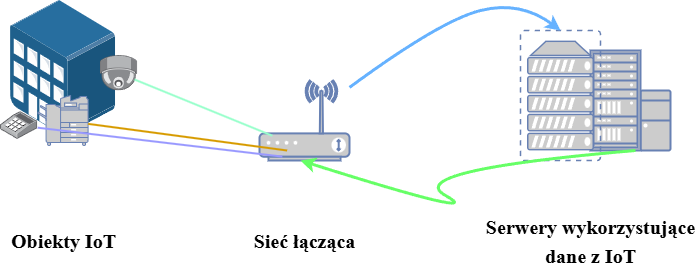
\includegraphics[width=0.8\textwidth]{pictures/IoT_basic.drawio.png}
    \caption{Trzy główne elementy IoT}
    \label{fig:Trzy główne elementy IoT}
\end{figure}

\vspace{1cm}

\textbf{Znaczenie IoT w różnych dziedzinach życia i gospodarki}
    \begin{itemize}
    \item \textbf{Gospodarka i Przemysł 4.0} – Internet Rzeczy jest kluczowym elementem transformacji cyfrowej przemysłu, znanej jako Przemysł 4.0. Dzięki integracji czujników i urządzeń z systemami produkcyjnymi możliwa jest ciągła analiza danych z maszyn, co pozwala przewidywać awarie, automatyzować linie produkcyjne oraz dynamicznie zarządzać zasobami. To z kolei przekłada się na zwiększenie wydajności, redukcję kosztów oraz poprawę jakości produktów.

    \item \textbf{Opieka zdrowotna} – IoT rewolucjonizuje sektor medyczny, umożliwiając zdalne monitorowanie pacjentów w czasie rzeczywistym, niezależnie od ich lokalizacji. Urządzenia noszone (np. smartwatche, inteligentne opaski) monitorują tętno, ciśnienie krwi, poziom cukru i inne parametry, przesyłając dane bezpośrednio do systemów lekarzy. Taka technologia znacząco zwiększa skuteczność leczenia przewlekłych chorób, poprawia jakość życia pacjentów oraz odciąża systemy opieki zdrowotnej.

    \item \textbf{Inteligentne miasta (Smart Cities)} – IoT umożliwia efektywne zarządzanie przestrzenią miejską i usługami publicznymi. Przykładowo, inteligentne systemy zarządzania ruchem drogowym pozwalają zmniejszyć korki i emisję spalin, a czujniki jakości powietrza umożliwiają monitorowanie poziomu zanieczyszczeń w czasie rzeczywistym. Oświetlenie uliczne może automatycznie dostosowywać natężenie światła w zależności od ruchu, co zmniejsza zużycie energii. Dzięki IoT miasta stają się bardziej przyjazne mieszkańcom, zrównoważone i nowoczesne.

    \item \textbf{Inteligentne domy (Smart Homes)} – W sferze prywatnej IoT zapewnia wygodę i bezpieczeństwo. Użytkownicy mogą zdalnie sterować systemami ogrzewania, klimatyzacji, oświetlenia czy domowymi urządzeniami elektronicznymi za pomocą smartfonów lub asystentów głosowych. Inteligentne zamki, alarmy i kamery zwiększają poziom ochrony, a automatyzacja procesów (np. harmonogramy włączania urządzeń) prowadzi do oszczędności energii i niższych rachunków.

    \item \textbf{Transport i logistyka} – Dzięki IoT firmy transportowe i logistyczne mogą śledzić pojazdy, monitorować warunki transportu (np. temperaturę w chłodniach), przewidywać opóźnienia oraz optymalizować trasy w czasie rzeczywistym. Technologie takie jak RFID i GPS w połączeniu z platformami analitycznymi pozwalają na dokładniejsze zarządzanie łańcuchem dostaw, redukując straty i zwiększając niezawodność dostaw.

    \item \textbf{Rolnictwo (Smart Agriculture)} – IoT ma ogromny potencjał w rolnictwie precyzyjnym. Czujniki gleby, stacje pogodowe i drony umożliwiają rolnikom monitorowanie warunków środowiskowych i upraw, automatyzację nawadniania czy kontrolę nad nawożeniem. Dzięki temu możliwe jest zwiększenie plonów, zmniejszenie zużycia wody i środków chemicznych oraz ograniczenie wpływu na środowisko. Systemy te wspierają także monitorowanie stanu zdrowia zwierząt hodowlanych, co przekłada się na lepszą jakość i efektywność produkcji \cite{wolfert2017big}.
\end{itemize}

\section{Kluczowe pojęcia związane z prywatnością i bezpieczeństwem danych w IoT}
\textbf{Prywatność} w systemach IoT odnosi się do ochrony danych osobowych użytkowników, ich anonimowości oraz metadanych zbieranych przez urządzenia IoT. W kontekście IoT prywatność zyskuje szczególne znaczenie, ponieważ urządzenia te często gromadzą bardzo wrażliwe informacje — na przykład dane zdrowotne, lokalizacyjne, czy osobiste preferencje użytkowników. Ponieważ wiele urządzeń łączy się z chmurą i innymi systemami w sieci, zagrożenia związane z niewłaściwym zarządzaniem tymi danymi są wysokie.

W praktyce zapewnienie prywatności oznacza wdrożenie odpowiednich polityk ochrony danych, takich jak zgodność z regulacjami prawnymi (np. RODO w Europie). Ważne jest stosowanie mechanizmów szyfrowania danych zarówno podczas transmisji, jak i ich przechowywania, aby uniemożliwić dostęp osobom nieuprawnionym. Równie istotna jest transparentność wobec użytkowników — powinni oni być informowani, jakie dane są zbierane, w jaki sposób są wykorzystywane i komu mogą być udostępniane. Ponadto, użytkownicy powinni mieć realną kontrolę nad swoimi danymi, np. możliwość ich usunięcia lub zmiany zgód na przetwarzanie.

\textbf{Bezpieczeństwo} danych w systemach IoT to szeroki zakres działań mających na celu ochronę integralności, poufności oraz dostępności informacji. Ze względu na rozproszoną architekturę IoT i ogromną liczbę połączonych urządzeń, systemy te są szczególnie podatne na różnorodne ataki. Do najczęstszych należą: manipulacja danymi, nieautoryzowany dostęp do urządzeń i sieci, ataki DDoS (Distributed Denial of Service), które przeciążają systemy, a także wstrzykiwanie złośliwego oprogramowania (malware), które może przejąć kontrolę nad urządzeniem lub całym systemem.

Aby przeciwdziałać tym zagrożeniom, kluczowe jest stosowanie zaawansowanych mechanizmów ochrony, takich jak:
\begin{itemize}
    \item \textbf{Szyfrowanie} - Zabezpieczenie danych przed przechwyceniem i odczytaniem.

    \item \textbf{Uwierzytelnianie} - Weryfikacja tożsamości urządzeń i użytkowników.
    
    \item \textbf{Zarządzanie tożsamościami i uprawnieniami} - Nadawanie odpowiednich ról i dostępów.
    
    \item \textbf{Monitorowanie i wykrywanie zagrożeń } - Ciągłe śledzenie zachowań w sieci i szybkie reagowanie na anomalie.
\end{itemize}

\textbf{Protokoły komunikuacyjne w systemach IoT} odgrywają kluczową rolę, umożliwiając urządzeniom wymianę danych i współpracę w sieci. Protokoły te są lekkie i energooszczędne, dostosowane do ograniczonych zasobów urządzeń. Można wyróżnić kilka kluczowych protokołów, takich jak: MQTT, CoAP, BLE, LoRaWAN.

\section{Różnorodność urządzeń IoT}
Systemy IoT integrują heterogeniczne urządzenia, które można sklasyfikować według dwóch kluczowych kryteriów:

\subsubsection{Klasyfikacja według zasobów obliczeniowych:}
    \begin{enumerate}
        \item \textbf{Urządzenia wysokiej mocy}: \\
        Urządzenia tego typu dysponują dużą mocą obliczeniową, często posiadają własne systemy operacyjne, wsparcie dla wielu protokołów komunikacyjnych i są zdolne do lokalnego przetwarzania danych bez konieczności stałego połączenia z chmurą.
        \begin{itemize}
            \item \textbf{Przykłady}: Roboty przemysłowe, serwery brzegowe (edge servers), bramki IoT (gateway), systemy SCADA (Supervisory Control and Data Acquisition), systemy MES (Manufacturing Execution Systems), sterowniki PLC (Programmable Logic Controllers). 
            \item \textbf{Zastosowania}: Lokalna analiza danych w czasie rzeczywistym (edge computing), agregacja danych z wielu czujników i ich przesyłanie do chmury, sterowanie złożonymi procesami przemysłowymi, reakcja na krytyczne zdarzenia bez opóźnień związanych z przesyłem do chmury.
            \item \textbf{Wyzwania bezpieczeństwa}: Ataki na interfejsy i protokoły (na podatne API lub niezabezpieczone porty), luki w aktualizacjach oprogramowania (brak automatycznych aktualizacji), ataki DDoS/DoS (przeciążenie bramki lub serwera brzegowego), złośliwe oprogramowanie.
        \end{itemize}
        \item \textbf{Urządzenia ograniczone zasobowo}: \\
        To małe, często jednozadaniowe urządzenia, które charakteryzują się niskim poborem mocy i ograniczoną pamięcią oraz mocą obliczeniową.
        \begin{itemize}
            \item \textbf{Przykłady}: Czujniki temperatury, wilgotności, ruchu, tagi RFID, urządzenia noszone (wearables), smartwatche, pompy insulinowe, inteligentne zamki, inteligentne termostaty. Zbieranie danych z otoczenia (np. środowiska, biometrycznych), identyfikacja i śledzenie (np. za pomocą RFID), zarządzanie energią i zużyciem w budynkach (smart building), monitorowanie stanu zdrowia w czasie rzeczywistym.
            \item \textbf{Wyzwania bezpieczeństwa}: Brak mocy obliczeniowej do implementacji zaawansowanych protokołów kryptograficznych, brak możliwości aktualizacji firmware'u, co utrudnia łatanie luk bezpieczeństwa, podatność na ataki fizyczne ze względu na mały rozmiar i łatwy dostęp, podatność na sniffing i spoofing w przypadku niezabezpieczonej komunikacji, ataki na lekkie protokoły komunikacyjne.
        \end{itemize}
    \end{enumerate}
    
\subsubsection{Klasyfikacja według funkcjonalności:}
    \begin{enumerate}
        \item \textbf{Sensory:} \\
        Urządzenia te służą do akwizycji danych – mierzą parametry otoczenia i przesyłają dane do centrów przetwarzania (lokalnych lub chmurowych).
        \begin{itemize}
            \item Zasosowania: Monitorowanie (np. jakości powietrza, wilgotności, ciśnienia), czujniki biomedyczne (np. EKG, ciśnieniomierze), systemy inteligentnych miast (np. monitoring hałasu, ruchu drogowego). 
            \item Podatności: Sensor spoofing (atak polegający na fałszowaniu danych np. podgrzanie czujnika), side-channel attacks (analiza poboru mocy, zakłóceń elektromagnetycznych w celu odczytu danych), fałszowanie danych wejściowych, które mogą wprowadzać błędy w całych systemach decyzyjnych.
        \end{itemize}
        \item \textbf{Aktuatory:} \\
        Urządzenia, które wykonują konkretne działania w odpowiedzi na dane wejściowe – mogą np. otworzyć zawór, uruchomić alarm lub zmienić ustawienia systemu.
        \begin{itemize}
            \item \textbf{Zasosowania}: Sterowanie np. oświetleniem, temperaturą, systemami bezpieczeństwa, reakcja na sytuacje awaryjne (np. włączenie alarmu przeciwpożarowego), automatyczne serowanie procesami przemysłowymi.
            \item \textbf{Podatności}: False data injection (wstrzyknięcie fałszywych danych skutkuje wykonaniem błędnych działań np. wyłączenie zabezpieczenia), ataki na protokoły komunikacyjne (np. przejęcie komunikacji między kontrolerem a aktuatorami), przejęcie kontroli nad urządzeniem (np. odblokowanie drzwi przez nieautoryzowanego użytkownika) \cite{antonakakis2017mirai}.
        \end{itemize}
        \item \textbf{Urządzenia hybrydowe:} \\
        Urządzenia łączące funkcje zarówno sensoryczne, jak i aktuacyjne — zbierają dane i na ich podstawie wykonują akcje.
        \begin{itemize}
            \item \textbf{Zasosowania}: Termostaty, które mierzą temperaturę i odpowiednio sterują ogrzewaniem, roboty mobilne, które analizują otoczenie i reagują (np. zmieniają trasę), Systemy automatyki domowej i przemysłowej.
            \item \textbf{Podatności}: Podwójna powierzchnia ataku (zarówno sensor, jak i aktuator mogą być celem - zwiększona ilośc potencjalnych obiektów ataku), złożoność urządzenia może powodować większe ryzyko błędów w konifguracji lub oprogramowani, synchornizacja ataków (np. jednoczesne przejęcie danych z czujnika i wprowadzenie błędnych działań poprzez aktuator).
        \end{itemize}
    \end{enumerate}
Przykłady urządzeń z każdej z powyższych kategorii funkcjonalnych przedstawiono na zdjęciach poniżej \ref{fig:Przykładowy sensor, aktuator i urządzenie hybrydowe}. Wszystkie zdjęcia zostały pozyskane ze stron producentów. Od lewej umieszczono: Sensor MAX30102, wykorzystujący technologię I2C, mierzy tętno i saturację (SpO2), znajduje zastosowanie w urządzeniach noszonych (monitorujących zdrowie). Następnym urządzeniem jest aktuator Shelly 2.5, który jest przekaźnikiem z funkcją pomiaru energii, umożliwiającym zdalne sterowanie np. oświetleniem, ogrzewaniem lub gniazdkami. Po prawej stronie znajduje się robot sprzątający Xiaomi Vacuum S20+, który jest przykładem urządzenia hybrydowego. Posiada funkcje sensoryczne w postaci mapowania pomieszczeń, wykrywania przeszkód oraz funkcje aktuacyjne - ruch, odkurzanie, nawigacja.
\begin{figure}[h]
    \centering
    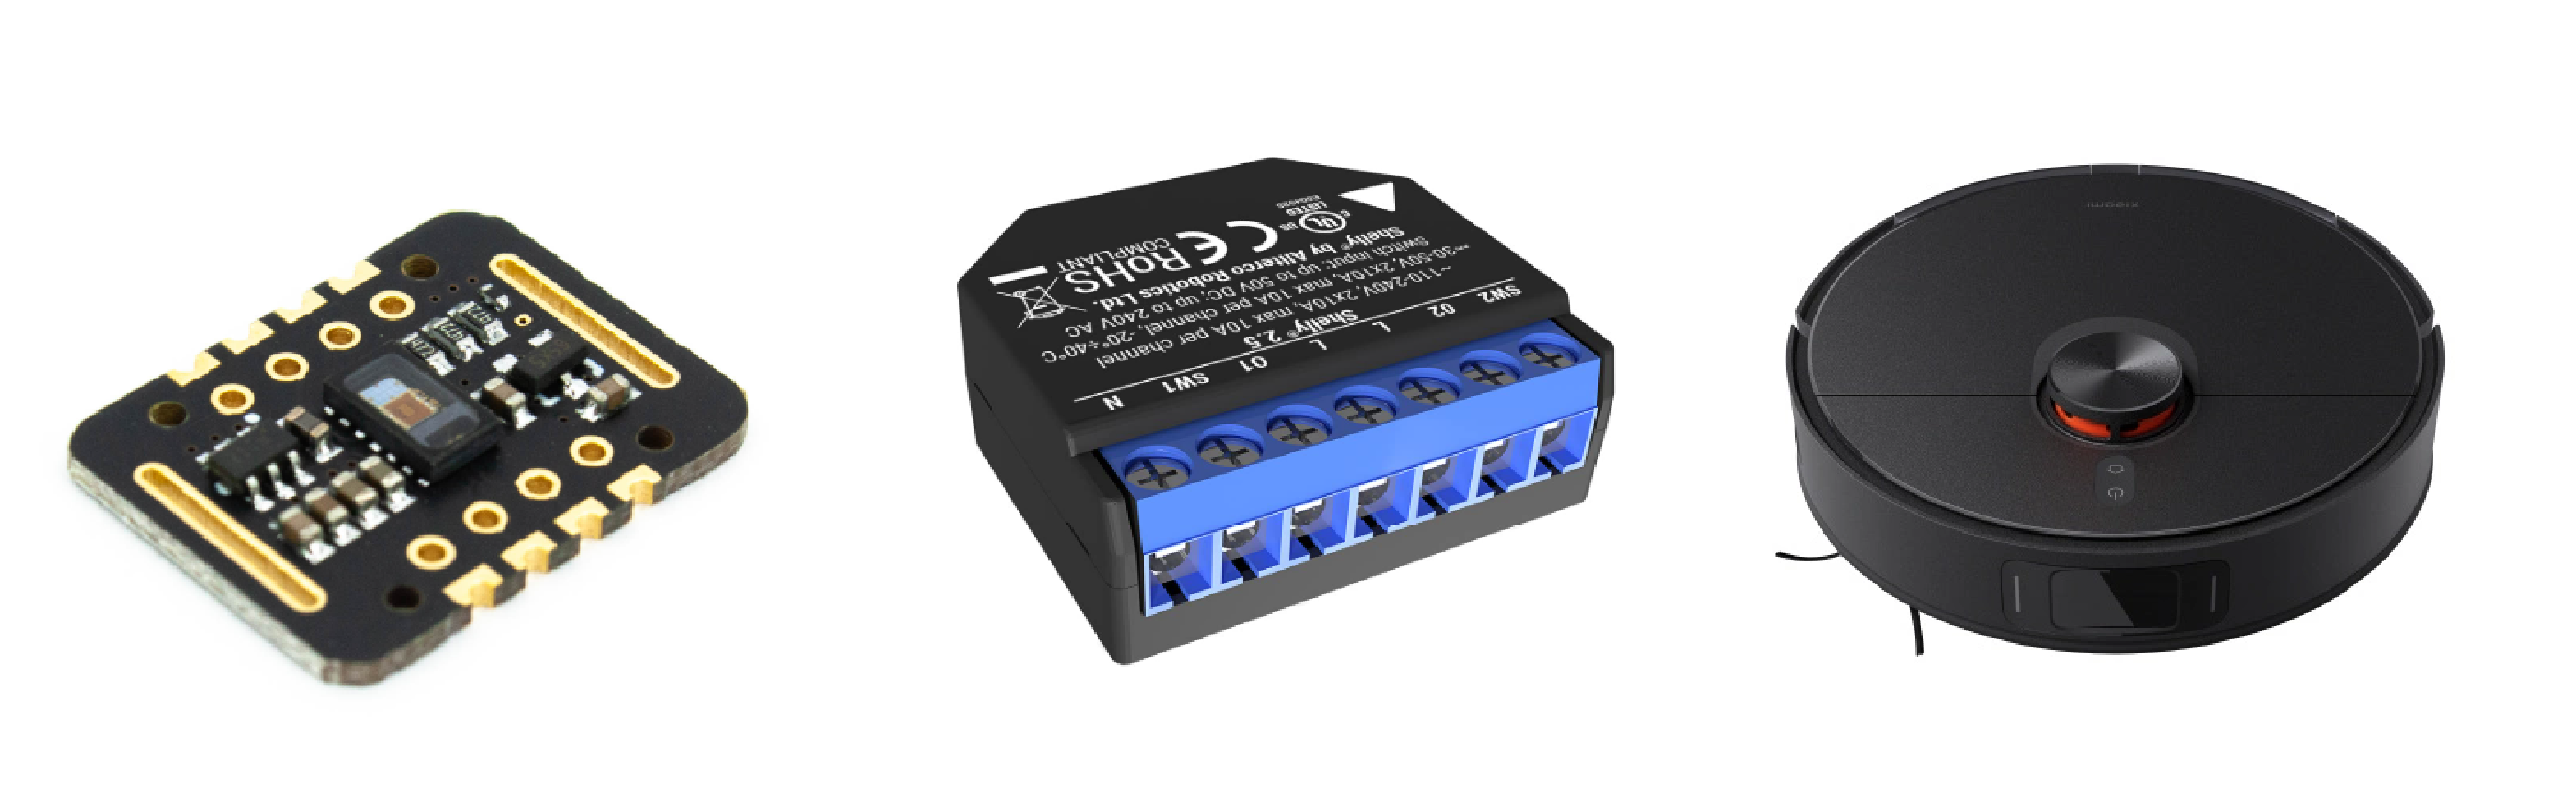
\includegraphics[width=0.8\textwidth]{pictures/urzadzenia-iot.png}
    \caption{Przykładowy sensor, aktuator i urządzenie hybrydowe}
    \label{fig:Przykładowy sensor, aktuator i urządzenie hybrydowe}
\end{figure}

\section{Architektury systemów IoT i ich implikacje bezpieczeństwa}

W systemach IoT wyróżnia się kilka architektur, które mają różne zalety i wady, zwłaszcza pod kątem bezpieczeństwa. Każda z tych architektur wprowadza unikalne wyzwania, które mogą wpływać na stabilność, prywatność i integralność danych. Ogólna architektura IoT przedstawiona jest na rysunku \ref{fig:Ogólna architektura IoT}.

\begin{figure}[h]
    \centering
    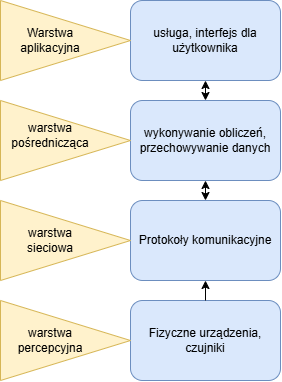
\includegraphics[width=0.3\textwidth]{pictures/IoTarch.drawio.png}
    \caption{Ogólna architektura IoT}
    \label{fig:Ogólna architektura IoT}
\end{figure}

\textbf{3-warstwowa architektura:}
Jest to podstawowy model IoT, który dzieli system na trzy główne warstwy: percepcyjną (obejmuje czujniki, urządzenia aktorów i inne komponenty zbierające dane), sieciową (odpowiada za przesył danych np. Wi-Fi, Bluetooth, LoRaWAN, 5G) i aplikacyjną (przetwarza dane i zapewnia interfejs użytkownikowi). Chociaż model ten jest prosty w implementacji, stanowi cel ataków typu Man-in-the-Middle (atakujący może przechwycić dane) w warstwie sieciowej oraz ataków na interfejsy użytkownika (np. SQL Injection) w warstwie aplikacyjnej. Ataki te mogą prowadzić do przechwycenia lub manipulacji danymi, a także przejęcia kontroli nad systemem.

\textbf{Architektura Edge Computing:}
W tej architekturze przetwarzanie danych odbywa się bezpośrednio na urządzeniach brzegowych (np. inteligentnych kamerach, sterownikach PLC), co pozwala na minimalizację opóźnień. Choć jest to ogromna zaleta, wprowadza również wyzwania związane z fizycznym bezpieczeństwem urządzeń. Ataki fizyczne, takie jak manipulacja urządzeniami lub ich fizyczne usunięcie, mogą być szczególnie groźne. Dodatkowo, ze względu na ograniczone zasoby urządzeń brzegowych, często stosuje się lekkie protokoły komunikacyjne, co może zwiększyć ryzyko ataków \cite{Lynn2020}.

\textbf{Architektura Fog Computing:}
Fog Computing stanowi pomost między urządzeniami brzegowymi (Edge) a chmurą, z wykorzystaniem węzłów przetwarzających dane lokalnie (Fog Nodes). Choć poprawia to wydajność, wprowadza nowe zagrożenia, takie jak ataki typu DDoS na węzły przetwarzające oraz problemy z zarządzaniem tożsamościami w rozproszonym środowisku \cite{Lynn2020}. W szczególności, bezpieczeństwo zarządzania tożsamością i dostępem w tej architekturze stanowi jedno z kluczowych wyzwań, szczególnie w kontekście dużych, heterogenicznych systemów \cite{OpenFog2018}.

\textbf{5-warstwowa architektura:}
Jest to rozwinięcie modelu 3-warstwowego o dodatkowe warstwy: przetwarzania (Edge/Fog Computing) oraz warstwę biznesową. Wprowadza to nowe możliwości, ale także dodatkowe wektory ataku. Przetwarzanie danych na brzegu sieci zmniejsza opóźnienia, ale wymaga odpowiednich zabezpieczeń rozproszonych węzłów przetwarzających. Warstwa biznesowa, odpowiedzialna za analizę danych oraz podejmowanie decyzji, narażona jest na ryzyko wycieku wrażliwych danych, co szczególnie dotyczy systemów, które muszą być zgodne z regulacjami, takimi jak RODO \cite{rao2023iot}.

\textbf{Architektura Cloud-Centric:}
W tej architekturze całość przetwarzania danych odbywa się w chmurze publicznej, co umożliwia dostęp do zaawansowanych narzędzi analitycznych i dużej mocy obliczeniowej. Jednak ta centralizacja danych wiąże się z ryzykiem, zwłaszcza w przypadku nieprawidłowo skonfigurowanych zasobów. Dodatkowo, ograniczenia konkretnego dostawcy chmurowego mogą ograniczyć elastyczność systemu i uniemożliwić łatwą migrację do innych platform.

\textbf{Architektura Peer-to-Peer (P2P):}
Architektura P2P eliminuje pośrednictwo chmury, zapewniając bezpośrednią komunikację między urządzeniami. Dzięki temu użytkownicy zyskują większą prywatność, ponieważ dane nie są przechowywane w centralnych zasobach. Niemniej jednak, brak centralnej kontroli utrudnia implementację skutecznych mechanizmów uwierzytelniania i audytu. Ponadto, w tej architekturze istnieje ryzyko ataków typu Sybil oraz manipulacji danymi, szczególnie w sieciach o niskim poziomie zaufania. Architektura P2P sprawdza się szczególnie w zastosowaniach wymagających niskich opóźnień, takich jak komunikacja między pojazdami.

Szczegółowe porównanie omówionych architektur pod kątem ich cech, zagrożeń i rozwiązań bezpieczeństwa prezentuje tabela \ref{tab:iot_architectures}.

\begin{landscape}
\renewcommand{\arraystretch}{1.5}
\begin{table}[h]
\centering
\caption{Porównanie architektur IoT pod kątem bezpieczeństwa}
\label{tab:iot_architectures}
\begin{tabular}{|l|l|l|l|}
\hline
\textbf{Architektura} & \textbf{Kluczowe cechy} & \textbf{Główne zagrożenia} & \textbf{Rozwiązania bezpieczeństwa} \\ \hline
3-warstwowa & 
\begin{tabular}[c]{@{}l@{}}- Percepcyjna\\ - Sieciowa\\ - Aplikacyjna\end{tabular} &
\begin{tabular}[c]{@{}l@{}}- MITM\\ - Ataki na interfejs\\ - Brak szyfrowania\end{tabular} &
\begin{tabular}[c]{@{}l@{}}- TLS\\ - Uwierzytelnianie MFA\end{tabular} \\ \hline

Edge Computing & 
\begin{tabular}[c]{@{}l@{}}- Przetwarzanie na brzegu\\ - Niskie opóźnienia\end{tabular} &
\begin{tabular}[c]{@{}l@{}}- Ataki fizyczne\\ - Ograniczone zasoby\\ - Ataki na firmware\end{tabular} &
\begin{tabular}[c]{@{}l@{}}- TPM\\ - Aktualizacje firmware\end{tabular} \\ \hline

Fog Computing & 
\begin{tabular}[c]{@{}l@{}}- Węzły przetwarzające\\ - Pośrednia warstwa\end{tabular} &
\begin{tabular}[c]{@{}l@{}}- DDoS\\ - Problemy z tożsamością\end{tabular} &
\begin{tabular}[c]{@{}l@{}}- Blockchain\\ - Detekcja anomalii\end{tabular} \\ \hline

5-warstwowa & 
\begin{tabular}[c]{@{}l@{}}- Dodana warstwa\\ przetwarzania i biznesowa\end{tabular} &
\begin{tabular}[c]{@{}l@{}}- Wyciek danych\\ - Ataki na węzły\end{tabular} &
\begin{tabular}[c]{@{}l@{}}- Szyfrowanie E2E\\ - RBAC\end{tabular} \\ \hline

Cloud-Centric & 
\begin{tabular}[c]{@{}l@{}}- Przetwarzanie w chmurze\\ - Duża moc obliczeniowa\end{tabular} &
\begin{tabular}[c]{@{}l@{}}- Błędy konfiguracji\\ - Vendor lock-in\end{tabular} &
\begin{tabular}[c]{@{}l@{}}- CSPM\\ - Multi-cloud\end{tabular} \\ \hline

Peer-to-Peer & 
\begin{tabular}[c]{@{}l@{}}- Bezpośrednia komunikacja\\ - Wysoka prywatność\end{tabular} &
\begin{tabular}[c]{@{}l@{}}- Ataki Sybil\\ - Brak audytu\end{tabular} &
\begin{tabular}[c]{@{}l@{}}- Mechanizmy reputacji\\ - Blockchain\end{tabular} \\ \hline
\label{tab:architektury-iot}
\end{tabular}
\end{table}
\end{landscape}
\section{Wprowadzenie do zagrożeń w systemach IoT}
Internet Rzeczy (IoT) niesie za sobą wiele korzyści, jednak dynamiczny rozwój tej technologii wiąże się także z licznymi zagrożeniami dla bezpieczeństwa i prywatności użytkowników. Ataki na urządzenia IoT mogą prowadzić do kradzieży danych, zakłóceń w działaniu systemów, a nawet fizycznych uszkodzeń infrastruktury. Poniżej przedstawiono najważniejsze zagrożenia związane z IoT.
\vspace{10pt} \\
\textbf{1. Nieautoryzowany dostęp} do urządzeń IoT to jedno z najczęściej występujących i najgroźniejszych zagrożeń w tym ekosystemie. Głównym powodem tej podatności jest fakt, że wiele urządzeń IoT jest dostarczanych z domyślnymi danymi logowania (np. „admin/admin”), które użytkownicy rzadko zmieniają. Co więcej, część producentów nie umożliwia nawet łatwej zmiany danych uwierzytelniających, co znacznie utrudnia zabezpieczenie tych urządzeń. Taka sytuacja sprzyja atakom typu brute-force, a także wykorzystaniu wcześniej wyciekłych danych logowania dostępnych w sieci.

Atak typu \textbf{brute force (siłowy)} polega na systematycznym próbowaniu wszystkich możliwych kombinacji nazw użytkowników i haseł, aż do momentu uzyskania poprawnych danych logowania. Jest to jeden z najprostszych, ale nadal skutecznych typów ataków, szczególnie w środowisku IoT.

Nieautoryzowany dostęp może mieć poważne skutki w różnych kontekstach środowisk domowych, przemysłowych lub medycynie. W środowiskach domowych, cyberprzestępcy mogą przejąć kontrolę nad inteligentnymi zamkami, systemami alarmowymi, kamerami monitoringu, termostatami czy asystentami głosowymi. Prowadzi to nie tylko do utraty prywatności, ale również może umożliwić fizyczne włamanie do domu bez śladów. W zastosowaniach przemysłowych przejęcie kontroli nad urządzeniami może prowadzić do sabotażu produkcji, awarii maszyn, błędów pomiarowych, a nawet stanowić zagrożenie dla życia pracowników. Szczególnie narażone są systemy SCADA, które często komunikują się bez odpowiedniego szyfrowania i uwierzytelniania. W medycynie nieautoryzowany dostęp do urządzeń medycznych (np. pomp infuzyjnych, monitorów EKG) może prowadzić do nieprawidłowego podania leków lub fałszywych odczytów parametrów życiowych, co może bezpośrednio zagrozić życiu pacjentów. \cite{antonakakis2017mirai}
\vspace{10pt} \\
\textbf{2. Śledzenie użytkowników}, urządzenia Internetu Rzeczy są często wyposażone w sensory i moduły komunikacyjne, które zbierają i przekazują dane dotyczące lokalizacji, aktywności fizycznej, nawyków użytkownika, a nawet parametrów zdrowotnych. Choć dane te są wykorzystywane do poprawy komfortu życia, personalizacji usług czy zwiększenia funkcjonalności urządzeń, to w przypadku niewystarczającej ochrony stają się one poważnym zagrożeniem dla prywatności użytkowników. Istnieje kilka sposobów, w jaki sposób może dochodzić do śledzenia:
\begin{itemize}
    \item \textbf{Analiza ruchu sieciowego} - Nawet jeśli dane są szyfrowane, analiza metadanych (częstotliwości połączeń, adresów IP, wzorców komunikacji) może zdradzić lokalizację lub zachowania użytkownika. \textit{Przykład: } Smartwatch regularnie łączy się z siecią Wi-Fi domową, a następnie z siecią biurową – łatwo wywnioskować miejsce zamieszkania i pracy.
    \item \textbf{Przechwytywanie sygnałów radiowych} -  Urządzenia IoT emitują sygnały Bluetooth, Zigbee, Wi-Fi — te mogą zostać przechwycone zdalnie. \textit{Przykład: } napastnik może ustalić obecność konkretnej osoby w danym miejscu, analizując emisję sygnału opaski fitness.
    \item \textbf{Podatności sprzętowe i firmware'owe} - Niektóre urządzenia posiadają luki w oprogramowaniu, które pozwalają na zdalne odczytywanie współrzędnych GPS lub danych z żyroskopów/akcelerometrów. \textit{Przykład: } inteligentny lokalizator samochodu, który przesyła dane bez szyfrowania – każdy z dostępem do sieci może je odczytać.
    \item \textbf{Nieświadoma zgoda użytkownika} - Aplikacje mobilne zbierają dane, których użytkownicy nie są w pełni świadomi (np. historia połączeń Bluetooth, logi z czujników). Dane te są często agregowane, sprzedawane lub przekazywane podmiotom trzecim (np. firmom reklamowym).
\end{itemize}
Skutkami śledzenia może być inwigilacja, stalking cyfrowy, kradzież tożsamości, czy profilowanie behawioralne. Jednym z najbardziej znanych ataków przeprowadzancyh w celu śledzenia użytkowników jest atak Man-in-the-Middle.
\vspace{10pt} \\
\textbf{3. Ataki typu Man-in-the-Middle (MITM)} polega na przechwyceniu i ewentualnej modyfikacji danych wymienianych pomiędzy dwoma stronami komunikacji — np. między urządzeniem IoT a serwerem w chmurze lub aplikacją mobilną użytkownika. W klasycznym scenariuszu atakujący „podszywa się” jednocześnie pod obie strony, nie ujawniając swojej obecności. W kontekście Internetu Rzeczy MITM jest szczególnie groźny, ponieważ wiele urządzeń korzysta z uproszczonych, lekkich protokołów komunikacyjnych, nie wdraża domyślnie szyfrowania (lub robi to w sposób nieprawidłowy), często działa na otwartych lub słabo zabezpieczonych środowiskach. W pierwszej fazie takiego ataku napastnik uzyskuje dostęp do sieci, w której znajduje się urządzenie IoT (np. poprzez niezabezpieczone Wi-Fi), po czym ustawia swoje urządzenie jako pośrednik między ofiarą a serwerem. Następnie jeśli komunikacja nie jest szyfrowana, dane mogą być przechwycone „w czystej postaci” (np. loginy, hasła, dane lokalizacyjne). Możliwa jest także manipulacja danymi w locie — np. zmiana polecenia sterującego lub wartości z czujnika. Schemat działania tego ataku w kontekście inteligentnego domu zobrazowano na rysunku \ref{fig:Schemat ataku typu Man-in-the-Middle (MITM) w systemach IoT}.
\begin{figure}[h]
    \centering
    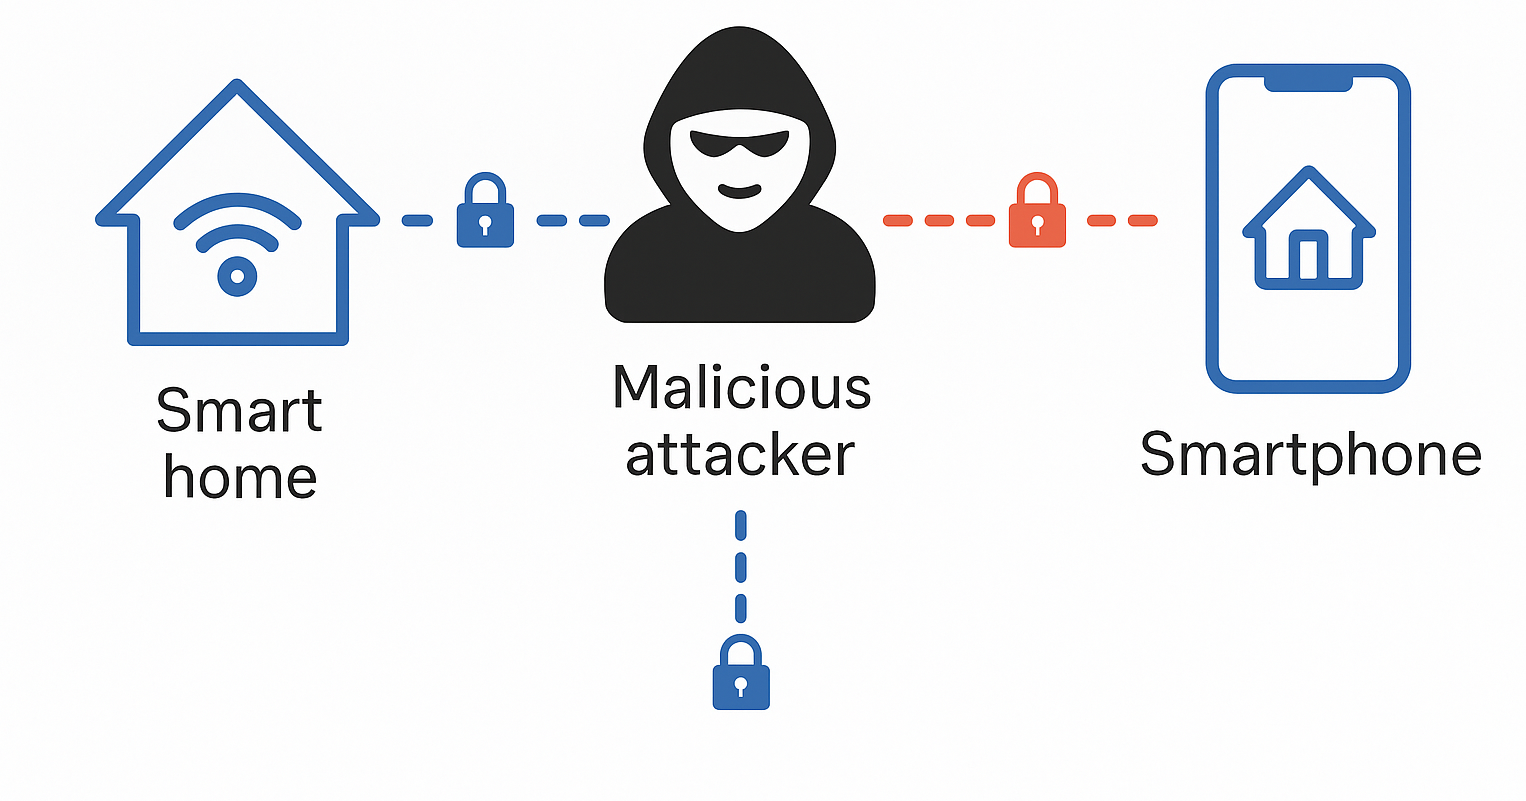
\includegraphics[width=0.6\textwidth]{pictures/MITM.png}
    \caption{Schemat ataku typu Man-in-the-Middle (MITM) w systemach IoT}
    \label{fig:Schemat ataku typu Man-in-the-Middle (MITM) w systemach IoT}
\end{figure}
\vspace{10pt} \\
\textbf{4. Manipulacja danymi} w systemach IoT stanowi jedno z bardziej podstępnych i trudnych do wykrycia zagrożeń, polegające na celowej zmianie, wstrzykiwaniu lub fałszowaniu przesyłanych danych. W przeciwieństwie do ataków ukierunkowanych na zakłócenie działania urządzeń, manipulacja danymi ma na celu wprowadzenie odbiorcy w błąd, co może prowadzić do błędnych decyzji systemów sterujących lub użytkowników.
W praktyce manipulacja danymi może przyjmować wiele form:
\begin{itemize}
    \item \textbf{Fałszowanie pomiarów} - w środowiskach medycznych może to oznaczać zmianę danych zbieranych przez czujniki monitorujące stan zdrowia pacjenta (np. tętno, ciśnienie krwi), co może prowadzić do niewłaściwej diagnozy i zagrożenia życia.
    \item \textbf{Sabotaż procesów przemysłowych} - atakujący mogą zmienić dane z czujników temperatury, ciśnienia lub wilgotności, co może doprowadzić do błędnych decyzji systemów automatyki i uszkodzenia maszyn lub całych linii produkcyjnych.
    \item \textbf{Zakłócenie systemów transportowych} - inteligentne systemy sterujące ruchem, bazujące na danych z wielu źródeł (czujniki, GPS, sygnalizacja), mogą zostać zmanipulowane, co może skutkować wypadkami, korkami lub nieprawidłowym sterowaniem ruchem.
    \item \textbf{Dezinformacja w systemach analitycznych} - manipulacja może dotyczyć np. danych środowiskowych (zanieczyszczenie powietrza, poziom hałasu), co może prowadzić do błędnych wniosków analitycznych i decyzji na poziomie zarządzania miastem.
    \item \textbf{Fałszywe alarmy i sabotaż} - w inteligentnych budynkach lub systemach zabezpieczeń zmiana danych z czujników (np. dymu, ruchu) może prowadzić do nieuzasadnionych alarmów, które dezorganizują pracę instytucji lub przedsiębiorstw.
\end{itemize}
Technicznie manipulacja danych może być przeprowadzona na różnych poziomach: ataki MITM, na poziomie samego urządzenia, na poziomie agregatorów danych, W systemach analitycznych lub bazach danych. Z uwagi na to, że IoT opiera się na automatycznym przetwarzaniu dużych ilości danych, ich integralność jest kluczowa. Nawet niewielka zmiana może spowodować poważne skutki w skali całego systemu \cite{schneier2018}.
\vspace{10pt} \\
\textbf{5. Ataki typu DDoS (Distributed Denial of Service) i DoS (Daniel of Service)} stanowią jedne z najpoważniejszych zagrożeń dla systemów Internetu Rzeczy. Ich celem jest zakłócenie lub całkowite uniemożliwienie działania danej usługi, aplikacji lub urządzenia, co może prowadzić do poważnych strat finansowych, przestojów w działaniu systemów oraz zagrożeń dla bezpieczeństwa użytkowników. 

Atak typu DoS polega na przeprowadzeniu przez jedno źródło (np. jedno urządzenie lub komputer) dużej liczby zapytań do danego systemu, serwera lub aplikacji w krótkim czasie. Celem jest przeciążenie zasobów docelowego systemu – takich jak pamięć, CPU lub pasmo sieciowe – aż do momentu, gdy stanie się on niedostępny dla legalnych użytkowników. Chociaż ataki DoS są relatywnie proste do zrealizowania, ich skuteczność w środowisku IoT jest większa z uwagi na ograniczoną moc obliczeniową i słabe zabezpieczenia wielu urządzeń. Przykład: prosty atak może skutecznie unieruchomić inteligentne czujniki, routery lub bramy IoT wykorzystywane np. w systemach monitoringu lub automatyki domowej.

DDoS to rozwinięcie ataku DoS, w którym udział bierze wiele rozproszonych źródeł – często setki tysięcy zainfekowanych urządzeń IoT. Tworzą one tzw. botnet, czyli sieć zombie – urządzeń zdalnie sterowanych przez atakującego.
Skutkami takich ataków w środowiskach IoT mogą być:
\begin{itemize}
    \item Zakłócenie działania infrastruktury krytycznej, np. systemów transportu, opieki zdrowotnej, automatyki przemysłowej.
    \item Straty finansowe wynikające z przestojów, kar umownych i konieczności przywracania usług.
    \item Utrata zaufania klientów i reputacji marki.
    \item Możliwość wykorzystania jako punktu wyjścia do innych, bardziej zaawansowanych ataków, takich jak manipulacja danymi czy kradzież informacji.
\end{itemize}

Przykładem z życia może być rekordowy atak DDoS w Polsce - W maju 2025 roku CERT Orange Polska odparł największy atak DDoS w historii polskiego internetu. Atak, który trwał kilka dni, osiągnął szczytowy ruch na poziomie 1,3 terabita na sekundę (Tbps). Dla porównania, przeciętne domowe łącze internetowe w Polsce ma przepustowość około 200 megabitów na sekundę (Mbps), co podkreśla skalę tego incydentu. \cite{certorange2025}
\vspace{10pt} \\
\textbf{6. Brak aktualizacji i podatności w oprogramowaniu}, wiele urządzeń IoT działa na oprogramowaniu, które nie jest regularnie aktualizowane, co znacząco zwiększa ryzyko wykorzystania znanych luk bezpieczeństwa. Producenci często nie zapewniają odpowiedniego wsparcia technicznego — w tym poprawek bezpieczeństwa czy aktualizacji systemów operacyjnych i firmware’u — przez co urządzenia pozostają narażone na ataki przez długi czas. Ponadto, nawet jeśli aktualizacje są dostępne, to użytkownicy często nie mają łatwej możliwości ich samodzielnego instalowania lub wręcz nie są świadomi potrzeby regularnej aktualizacji. W wielu przypadkach proces aktualizacji wymaga specjalistycznej wiedzy lub ingerencji serwisu, co powoduje, że aktualizacje są pomijane lub opóźniane. Brak regularnych aktualizacji powoduje, że urządzenia IoT stają się łatwym celem dla cyberprzestępców, którzy mogą wykorzystać istniejące podatności do przejęcia kontroli nad systemami, podsłuchiwania komunikacji, wprowadzania złośliwego oprogramowania lub tworzenia botnetów wykorzystywanych do ataków DDoS i innych działań przestępczych. W praktyce oznacza to, że nawet najnowsze i najbardziej zaawansowane urządzenia mogą stać się zagrożeniem, jeśli ich oprogramowanie nie jest odpowiednio i systematycznie zabezpieczane. W konsekwencji, brak aktualizacji nie tylko naraża prywatność i bezpieczeństwo użytkowników, ale może mieć również poważne skutki dla całej infrastruktury sieciowej \cite{johnston2019}.
\vspace{10pt} \\
\textbf{7. Ataki fizyczne} na urządzenia IoT to realne zagrożenie, szczególnie w przypadku systemów rozmieszczonych w przestrzeni publicznej, przemysłowej lub trudno nadzorowanej. Urządzenia IoT, takie jak czujniki, kamery, bramki komunikacyjne czy sterowniki PLC, często działają w niekontrolowanych środowiskach, co czyni je podatnymi na manipulacje fizyczne. Atakujący mogą uzyskać fizyczny dostęp do urządzenia w celu: zresetowania ustawień do wartości fabrycznych i przejęcia nad nim kontroli, podłączenia interfejsów debugowania (np. UART), aby uzyskać dostęp do firmware'u lub danych, zainstalowania złośliwego oprogramowania, wymiany komponentów elektronicznych lub podmiany całego urządzenia, zasilania urządzenia w celu obserwacji jego działania w bezpiecznym środowisku laboratoryjnym. W sektorach takich jak przemysł, transport czy smart city, skutki takich ataków mogą być poważne — od wycieku danych po sabotaż procesów operacyjnych. Przykładem może być manipulacja czujnikami w inteligentnych systemach sterowania ruchem lub dostęp do lokalnych węzłów sieci energetycznych. 
\vspace{10pt}
Internet Rzeczy wprowadza zasadnicze zmiany w sposobie gromadzenia i przetwarzania danych, jednocześnie tworząc nowe wektory potencjalnych ataków. Ograniczenia sprzętowe wielu urządzeń stanowią poważną barierę w implementacji zaawansowanych mechanizmów ochrony. Choć protokoły komunikacyjne są zoptymalizowane pod kątem wydajności, często okazują się niewystarczające w kontekście zapewnienia odpowiednich zabezpieczeń. 

% TODO
\chapter{Zabezpieczenia w systemach IoT}
\label{chap:rozdzial3}
\section{Przegląd zabezpieczeń stosowanych w systemach IoT}
Dynamiczny rozwój IoT pociąga za sobą liczne wyzwania z zakresu cyberbezpieczeństwa. Ze względu na ogromną liczbę urządzeń, różnorodność architektur oraz ograniczenia sprzętowe, projektowanie skutecznych zabezpieczeń w systemach IoT wymaga szczególnej uwagi.
W tej sekcji zostanie przedstawiony przegląd najważniejszych zabezpieczeń stosowanych w systemach IoT, które mają na celu ochronę danych, urządzeń oraz komunikacji w sieciach IoT.
\subsection{Szyfrowanie danych}
Jednym z podstawowych środków ochrony danych w systemach IoT jest szyfrowanie. Chroni ono informacje przesyłane między urządzeniami brzegowymi, bramkami a serwerami centralnymi przed nieautoryzowanym dostępem, modyfikacją lub podsłuchem. W środowisku IoT, gdzie często występują ograniczenia zasobów (moc obliczeniowa, pamięć, zużycie energii), wybór odpowiednich algorytmów szyfrujących jest kluczowy dla zachowania równowagi między bezpieczeństwem a wydajnością.

W praktyce stosuje się zarówno algorytmy szyfrowania symetrycznego, jak i asymetrycznego:
\begin{itemize}
    \item \textbf{AES (Advanced Encryption Standard)} – jest najczęściej stosowanym algorytmem szyfrowania symetrycznego w systemach IoT. Oferuje wysoki poziom bezpieczeństwa przy stosunkowo niskim zapotrzebowaniu na zasoby, co czyni go odpowiednim dla urządzeń o ograniczonych możliwościach. Typowe długości kluczy to 128, 192 lub 256 bitów. AES jest powszechnie wykorzystywany w transmisji danych, np. w komunikacji Bluetooth, Zigbee, LoRaWAN czy TLS.
    
    \item \textbf{RSA} – klasyczny algorytm kryptografii asymetrycznej, stosowany głównie do wymiany kluczy szyfrowania lub podpisów cyfrowych. Choć zapewnia wysoki poziom bezpieczeństwa, jego implementacja może być zbyt zasobożerna dla wielu małych urządzeń IoT.
    
    \item \textbf{ECC (Elliptic Curve Cryptography)} - nowocześniejsza alternatywa dla RSA. Dzięki mniejszym kluczom (np. 256-bitowy klucz ECC oferuje porównywalne bezpieczeństwo do 3072-bitowego RSA), ECC jest lepiej dostosowana do wymagań środowisk IoT. Jest szeroko stosowana w certyfikatach cyfrowych, podpisach oraz uwierzytelnianiu urządzeń \cite{nist_keylength}.
\end{itemize}

Dodatkowo, w zaawansowanych systemach stosuje się często połączenie obu podejść w tzw. kryptografii hybrydowej – asymetryczna kryptografia służy do bezpiecznej wymiany klucza sesyjnego, po czym dalsza komunikacja odbywa się z użyciem szyfrowania symetrycznego.

Warto również wspomnieć o istotnej roli zarządzania kluczami (key management), które w systemach rozproszonych, takich jak IoT, stanowi jedno z największych wyzwań w zakresie bezpieczeństwa. Niewłaściwe przechowywanie, dystrybucja lub rotacja kluczy może zniweczyć skuteczność nawet najsilniejszych algorytmów szyfrowania.

\subsection{Autoryzacja i uwierzytelnianie}
W systemach IoT krytyczne znaczenie ma zapewnienie, że jedynie uprawnione urządzenia oraz użytkownicy mają dostęp do zasobów i funkcji systemu. Ochrona przed nieautoryzowanym dostępem odbywa się na dwóch kluczowych poziomach:

\textbf{Uwierzytelnienie} - proces weryfikacji tożsamości użytkownika lub urządzenia. Ma na celu potwierdzenie, że dany podmiot jest tym, za kogo się podaje.
W środowisku IoT, gdzie urządzenia często komunikują się automatycznie bez udziału człowieka, uwierzytelnianie musi być zarówno bezpieczne, jak i lekkie obliczeniowo.
\begin{itemize}
    \item \textbf{Uwierzytelnianie dwuskładnikowe (2FA)} — stosowane najczęściej po stronie użytkowników końcowych, wymaga podania dwóch niezależnych elementów (np. hasła i kodu SMS lub aplikacji uwierzytelniającej). Zmniejsza ryzyko przejęcia konta nawet w przypadku kradzieży jednego składnika.
    
    \item \textbf{Certyfikaty X.509} — szeroko stosowane w komunikacji typu urządzenie-urządzenie (\textit{device-to-device}) oraz urządzenie-serwer (\textit{device-to-server}). Umożliwiają wzajemne uwierzytelnianie przy pomocy infrastruktury klucza publicznego (PKI). Certyfikaty te zawierają m.in. klucz publiczny, tożsamość właściciela oraz podpis urzędu certyfikacji (CA) \cite{stallings2017cryptography}.
    
    \item \textbf{Uwierzytelnianie oparte na kluczach symetrycznych} — wykorzystywane w urządzeniach o bardzo ograniczonych zasobach, gdzie przechowywany jest wspólny sekret. Rozwiązanie to jest wydajne, lecz trudniejsze w zarządzaniu w większych systemach z wieloma uczestnikami.
\end{itemize}
Po pomyślnym uwierzytelnieniu użytkownik lub urządzenie uzyskuje prawa dostępu do określonych zasobów systemu. Autoryzacja może być oparta na rolach, zasadach lub tokenach.

\textbf{Autoryzacja} - proces przyznawania uprawnień do określonych zasobów lub działań po uprzednim uwierzytelnieniu. Określa, co dany użytkownik lub urządzenie może zrobić w systemie.
\begin{itemize}
    \item \textbf{OAuth 2.0} — protokół autoryzacji, który pozwala aplikacjom zewnętrznym na dostęp do zasobów użytkownika bez potrzeby udostępniania hasła. Powszechnie używany w aplikacjach mobilnych i chmurowych \cite{hardt2012oauth}.
    
    \item \textbf{JWT (JSON Web Token)} — samopodpisany token zawierający dane o użytkowniku i jego uprawnieniach, używany w rozproszonych systemach IoT do autoryzacji żądań API \cite{jones2015jwt}.
\end{itemize}

\textbf{Modele autoryzacji RBAC i ABAC:}
\begin{itemize}
    \item \textbf{RBAC (Role-Based Access Control)} — użytkownicy przypisani są do ról, a role definiują dostęp do zasobów. Popularne w dużych systemach z wieloma użytkownikami.
    
    \item \textbf{ABAC (Attribute-Based Access Control)} — decyzje o dostępie podejmowane są na podstawie atrybutów użytkownika, zasobu oraz kontekstu (np. lokalizacji, czasu) \cite{sicari2015security}.
\end{itemize}

W praktyce, skuteczne zabezpieczenie systemów IoT wymaga stosowania obu mechanizmów — uwierzytelniania w celu potwierdzenia tożsamości oraz autoryzacji w celu kontroli dostępu. Wyzwania w tym zakresie obejmują m.in. skalowalność systemów zarządzania tożsamościami, ochronę prywatności użytkowników oraz ograniczenia sprzętowe wielu urządzeń końcowych.

\subsection{Zarządzanie tożsamością i integracja z systemami IAM}

Zarządzanie tożsamością (ang. Identity and Access Management, IAM) w środowisku IoT obejmuje procesy nadawania, kontrolowania i weryfikowania tożsamości zarówno użytkowników, jak i urządzeń. W praktyce oznacza to przypisywanie unikalnych identyfikatorów, nadawanie odpowiednich uprawnień oraz kontrolę dostępu do zasobów i usług w sposób zautomatyzowany i skalowalny \cite{microsoftIAM}.

IAM odgrywa kluczową rolę w:
\begin{itemize}
    \item zarządzaniu cyklem życia urządzeń (rejestracja, uwierzytelnianie, dezaktywacja),
    
    \item zapewnianiu spójnej polityki dostępu w zróżnicowanych środowiskach,
    
    \item integracji z chmurą, aplikacjami mobilnymi i systemami klasy enterprise.
\end{itemize}

\subsubsection*{Zarządzanie tożsamością użytkowników i integracja z korporacyjnymi systemami}

W organizacjach IoT często integrowane są z istniejącymi systemami IAM, co umożliwia centralne zarządzanie uprawnieniami i jednolite stosowanie polityk bezpieczeństwa.

\begin{itemize}
    \item \textbf{LDAP (Lightweight Directory Access Protocol)} – protokół umożliwiający przeszukiwanie i modyfikację danych w usługach katalogowych, takich jak OpenLDAP czy Active Directory. Używany do autoryzacji i uwierzytelniania użytkowników i urządzeń.
    
    \item \textbf{Active Directory} – usługa katalogowa firmy Microsoft, szeroko stosowana w środowiskach korporacyjnych. Może pełnić funkcję repozytorium tożsamości urządzeń IoT dzięki integracji z rozwiązaniami gatewayowymi i brokerami IoT \cite{microsoftIAMiot}.

    \item \textbf{SAML (Security Assertion Markup Language)} – standard wymiany uwierzytelnionych danych między podmiotami (identity providers i service providers). Umożliwia jednokrotne logowanie (SSO) i jest wykorzystywany np. przy integracji z aplikacjami chmurowymi \cite{microsoftSAML}.
    
    \item \textbf{OpenID Connect} – protokół uwierzytelniania oparty na OAuth 2.0, stosowany w nowoczesnych aplikacjach webowych i mobilnych. Coraz częściej wykorzystywany również w rozwiązaniach IoT z interfejsem użytkownika \cite{microsoftOIDC}.
\end{itemize}

\subsubsection*{Zarządzanie tożsamością urządzeń (IoT IAM)}

IAM dla urządzeń różni się znacząco od klasycznego IAM dla ludzi, ponieważ:

\begin{itemize}
    \item każde urządzenie musi mieć unikalną, trudną do podrobienia tożsamość,
    
    \item proces rejestracji i provisioning musi być możliwie zautomatyzowany,
    
    \item uprawnienia muszą być nadawane w sposób dynamiczny, często zależnie od lokalizacji, czasu lub stanu urządzenia.
\end{itemize}

Popularne podejścia obejmują:
\begin{itemize}
    \item \textbf{Zarządzanie certyfikatami (PKI)} – urządzenia identyfikowane na podstawie certyfikatów X.509 i kluczy kryptograficznych.
    
    \item \textbf{IAM-as-a-Service} – usługi chmurowe (np. AWS IoT Core, Azure IoT Hub) oferujące rejestrację, uwierzytelnianie i kontrolę dostępu jako usługę.
\end{itemize}

Efektywne IAM w IoT jest fundamentem zaufanego środowiska cyfrowego, w którym urządzenia i użytkownicy mogą bezpiecznie współpracować zgodnie z zasadą najmniejszych uprawnień.

\subsection{Protokoły komunikacyjne i ich zabezpieczenia}

W systemach IoT wykorzystywane są różnorodne protokoły komunikacyjne, dostosowane do specyfiki urządzeń, wymagań dotyczących zużycia energii oraz zakresu transmisji. Każdy z nich implementuje własne mechanizmy bezpieczeństwa, mające na celu ochronę danych przesyłanych między urządzeniami oraz zapobieganie atakom sieciowym.

\begin{itemize}
    \item \textbf{MQTT (Message Queuing Telemetry Transport)} – jest to lekki protokół publikacji/subskrypcji, zoptymalizowany pod kątem urządzeń o ograniczonych zasobach oraz sieci o niskiej przepustowości. MQTT sam w sobie nie posiada wbudowanych mechanizmów bezpieczeństwa, dlatego najczęściej stosuje się go w połączeniu z warstwą TLS (Transport Layer Security), która zapewnia szyfrowanie transmisji oraz uwierzytelnianie serwera. Dodatkowo, do zabezpieczenia dostępu do brokera MQTT stosowane są mechanizmy uwierzytelniania z wykorzystaniem nazw użytkowników i haseł, a także tokenów dostępu, co pozwala na kontrolę autoryzacji urządzeń \cite{light2017mqtt}.

    \item \textbf{CoAP (Constrained Application Protocol)} – protokół zaprojektowany dla sieci o ograniczonych zasobach, takich jak sensorowe sieci bezprzewodowe. CoAP działa na bazie UDP, co pozwala na niskie opóźnienia i minimalizację zużycia energii. Bezpieczeństwo w CoAP zapewnia protokół DTLS (Datagram Transport Layer Security), który dostarcza uwierzytelnianie, integralność i szyfrowanie danych przesyłanych przez UDP, chroniąc przed podsłuchiwaniem i modyfikacją komunikatów \cite{shelby2014constrained}.

    \item \textbf{Zigbee} – standard komunikacji bezprzewodowej dedykowany urządzeniom o niskim poborze energii i krótkim zasięgu. Zigbee oferuje zabezpieczenia na poziomie warstwy sieciowej i aplikacyjnej, m.in. szyfrowanie AES-128, uwierzytelnianie urządzeń oraz mechanizmy ochrony przed replay attack. Zarządzanie kluczami kryptograficznymi w Zigbee umożliwia dynamiczne tworzenie i dystrybucję kluczy, co zwiększa odporność na próby przechwycenia komunikacji \cite{zigbeeAlliance}.

    \item \textbf{LoRaWAN (Long Range Wide Area Network)} – protokół dedykowany długodystansowej komunikacji urządzeń IoT o bardzo niskim zużyciu energii. LoRaWAN zapewnia bezpieczeństwo na dwóch poziomach: warstwy sieciowej oraz aplikacyjnej. Uwierzytelnianie urządzeń odbywa się poprzez unikalne klucze sesji, a dane przesyłane są szyfrowane z wykorzystaniem algorytmu AES-128. Takie podejście chroni prywatność danych oraz zabezpiecza przed nieautoryzowanym dostępem do sieci \cite{adelantado2017understanding}.

    \item \textbf{Bluetooth Low Energy (BLE)} – protokół bezprzewodowej komunikacji krótkiego zasięgu, często stosowany w urządzeniach IoT osobistego użytku. BLE stosuje mechanizmy zabezpieczeń oparte na procesie parowania urządzeń, który może wykorzystywać różne metody uwierzytelniania, w tym kod PIN, Just Works, Numeric Comparison czy Passkey Entry. Po sparowaniu, komunikacja jest zabezpieczona szyfrowaniem linku, co chroni przed podsłuchiwaniem oraz ingerencją osób trzecich \cite{bleSpec}.

\end{itemize}

Warto podkreślić, że mimo wbudowanych mechanizmów zabezpieczeń, skuteczność ochrony zależy również od prawidłowej konfiguracji protokołów oraz stosowania najlepszych praktyk, takich jak regularna aktualizacja oprogramowania, zarządzanie kluczami kryptograficznymi i monitoring sieci. W dobie rosnącej liczby urządzeń IoT, zabezpieczenie komunikacji jest jednym z kluczowych elementów zapewniających integralność, poufność oraz dostępność systemów.
Szczegółowe zestawienie właściwości i zabezpieczeń najpopularniejszych protokołów IoT przedstawiono w tabeli \ref{tab:iot_protocols_security}.
\begin{landscape}
\vspace*{2cm}
\renewcommand{\arraystretch}{1.3} 
\setlength{\tabcolsep}{4pt} 
\begin{table}[htbp]
\centering
\small 
\caption{Porównanie protokołów komunikacyjnych i ich zabezpieczeń w systemach IoT}
\label{tab:iot_protocols_security}
\begin{tabular}{|l|l|l|p{4cm}|p{3.5cm}|l|l|}
\hline
\textbf{Protokoł} & \textbf{Typ transportu} & \textbf{Bezpieczeństwo} & \textbf{Mechanizmy zabezpieczeń} & \textbf{Zastosowanie} & \textbf{Zużycie energii} & \textbf{Zasięg}\cite{sicari2015security} \\ \hline
MQTT & TCP & TLS (SSL) & Uwierzytelnianie przez hasła, TLS & Telemetria, M2M, niskie opóźnienia & Niskie & Krótki / średni \\ \hline
CoAP & UDP & DTLS & Szyfrowanie DTLS, uwierzytelnianie & Sieci sensorowe, urządzenia ograniczone & Bardzo niskie & Krótki \\ \hline
Zigbee & IEEE 802.15.4 & AES-128 & Szyfrowanie, uwierzytelnianie, klucze sesji & Automatyka domowa, niskopoborowe urządzenia & Bardzo niskie & Krótki (10-100 m) \\ \hline
LoRaWAN & Sub-GHz radio & AES-128 & Uwierzytelnianie urządzeń, szyfrowanie danych & Długodystansowe IoT, niskie zużycie energii & Bardzo niskie & Długi (kilometry) \\ \hline
BLE & RF (2.4 GHz) & Szyfrowanie linku, parowanie & Parowanie, uwierzytelnianie, szyfrowanie & Wearables, IoT krótkiego zasięgu & Niskie & Krótki (do 100 m) \\ \hline
\label{tab:iot_protocols_security}
\end{tabular}
\end{table}
\end{landscape}



\subsection{Dodatkowe techniki zabezpieczeń w IoT}
Oprócz wymienionych wcześniej zabezpieczeń, w systemach IoT stosuje się również inne techniki, które mają na celu zwiększenie bezpieczeństwa:
\begin{itemize}
    \item \textbf{Segmentacja sieci} - polega na podziale sieci IoT na mniejsze, izolowane segmenty lub strefy bezpieczeństwa. Dzięki temu w przypadku naruszenia jednego segmentu atak nie rozprzestrzenia się na cały system, co minimalizuje ryzyko i ułatwia zarządzanie bezpieczeństwem.
    
    \item \textbf{Monitorowanie i analiza ruchu sieciowego} - zaawansowane systemy wykrywające anomalie i analityka ruchu sieciowego pozwalają na identyfikację nietypowych zachowań, potencjalnych prób ataku oraz wczesne reagowanie na zagrożenia. Coraz częściej wykorzystywane są metody oparte na uczeniu maszynowym do automatycznej detekcji nieprawidłowości.
    
    \item \textbf{Aktualizacej OTA (Over-The-Air)} - umożliwiają zdalne i bezpieczne dostarczanie poprawek oraz nowych wersji oprogramowania na urządzenia IoT bez konieczności fizycznej ingerencji. Kluczowe jest tu zabezpieczenie procesu aktualizacji, np. przez cyfrowe podpisy aktualizacji, aby zapobiec wgraniu złośliwego oprogramowania \cite{android_ota}.
    
    \item \textbf{Zaufany komponent (Trusted Platform Module, TPM)} - jest to sprzętowy moduł zabezpieczający, który przechowuje klucze kryptograficzne, certyfikaty i inne wrażliwe dane w izolowanym środowisku. TPM umożliwia m.in. bezpieczne generowanie kluczy, uwierzytelnianie urządzenia oraz zapewnia integralność systemu \cite{tpm}.
    
    \item \textbf{Bezpieczne bootowanie (Secure Boot)} – mechanizm, który zapewnia, że urządzenie uruchamia tylko zweryfikowane i autoryzowane oprogramowanie, co zapobiega uruchomieniu złośliwego kodu na poziomie startu systemu.
    
    \item \textbf{Hardware Security Modules (HSM)} – dedykowane, fizyczne urządzenia lub moduły zabezpieczające o wysokim poziomie ochrony, wykorzystywane do zarządzania kluczami kryptograficznymi oraz realizacji operacji kryptograficznych w bezpiecznym środowisku sprzętowym.
    
    \item \textbf{Zarządzanie cyklem życia urządzenia} – ścisła kontrola i monitorowanie urządzeń IoT od momentu produkcji, przez wdrożenie, eksploatację, aż do utylizacji, co pomaga zapobiegać wykorzystaniu podatnych lub nieautoryzowanych urządzeń w sieci.
\end{itemize}

\section{Wyzwania związane z prywatnością i bezpieczeństwem w IoT}
Wraz z rosnącą liczbą urządzeń IoT w życiu codziennym oraz sektorze przemysłowym, wzrasta liczba potencjalnych zagrożeń związanych z prywatnością użytkowników i bezpieczeństwem danych. Systemy te często operują w rozproszonym środowisku, gromadząc i przetwarzając duże ilości danych, w tym dane osobowe. W rezultacie pojawiają się nowe wyzwania, których nie sposób zignorować przy projektowaniu i wdrażaniu rozwiązań IoT.
\subsection{Wyciek danych osobowych}
Jednym z najpoważniejszych problemów związanych z Internetem Rzeczy (IoT) jest ryzyko wycieku danych osobowych. Urządzenia IoT, takie jak inteligentne kamery monitoringu, opaski fitness, asystenci głosowi czy inteligentne liczniki energii, na bieżąco zbierają ogromne ilości informacji o użytkownikach i ich otoczeniu. Dane te obejmują między innymi szczegółowe informacje o lokalizacji, stanie zdrowia, codziennych nawykach, preferencjach zakupowych, a także dane środowiskowe, które mogą pośrednio ujawniać informacje o stylu życia czy aktywnościach użytkownika.

Ze względu na specyfikę i często ograniczone zasoby urządzeń IoT, w tym ograniczoną moc obliczeniową i pamięć, zabezpieczenia danych mogą być niewystarczające lub nieaktualne.
Konsekwencje wycieku danych osobowych są wielowymiarowe. Poza bezpośrednim zagrożeniem dla prywatności użytkowników, mogą wystąpić także skutki prawne i finansowe dla producentów i operatorów urządzeń IoT. W Unii Europejskiej obowiązuje Rozporządzenie o Ochronie Danych Osobowych (RODO), które nakłada na firmy obowiązek odpowiedniego zabezpieczenia danych osobowych oraz zgłaszania incydentów naruszenia bezpieczeństwa danych w określonym czasie. Naruszenie tych przepisów może skutkować wysokimi karami finansowymi i utratą reputacji.
\subsection{Śledzenie aktywności użytkowników}
Urządzenia IoT coraz częściej stają się integralną częścią codziennego życia, dostarczając danych na temat aktywności, nawyków oraz zachowań swoich użytkowników. Takie dane mogą pochodzić z różnorodnych źródeł — inteligentnych zegarków, opasek fitness, asystentów głosowych, kamer monitoringu, systemów automatyki domowej czy nawet inteligentnych urządzeń AGD.

Gromadzenie i analiza tych informacji pozwala na dostarczanie spersonalizowanych usług, poprawę wygody użytkownika oraz optymalizację funkcjonowania urządzeń. Jednak równocześnie niesie to za sobą poważne zagrożenia związane z prywatnością i bezpieczeństwem:

\begin{itemize}
\item \textbf{Nieautoryzowane śledzenie} — jeżeli dane nie są odpowiednio chronione, osoby trzecie mogą przechwycić szczegółowe informacje dotyczące ruchów, lokalizacji i codziennych rutyn użytkownika. Może to prowadzić do profilowania oraz tworzenia dokładnych map zachowań.

\item \textbf{Brak przejrzystości i świadomej zgody} — często użytkownicy nie są w pełni informowani o tym, jakie dane są zbierane i w jakim celu, a proces uzyskiwania zgody bywa niejasny lub ukryty w długich i skomplikowanych regulaminach.

\item \textbf{Wykorzystanie danych do celów komercyjnych} — dane mogą być sprzedawane lub udostępniane firmom marketingowym, które na ich podstawie prowadzą ukierunkowane kampanie reklamowe, czasem bez wiedzy lub zgody użytkownika.

\item \textbf{Potencjalne wykorzystanie w celach przestępczych} — informacje o tym, kiedy użytkownicy są obecni lub nieobecni w domu, mogą zostać wykorzystane przez osoby o złych intencjach, np. do planowania włamań czy innych form nadużyć.

\item \textbf{Ryzyko inwigilacji} — w niektórych przypadkach dane zbierane przez IoT mogą być wykorzystywane przez organy państwowe lub inne podmioty do nadzoru nad obywatelami, co rodzi obawy dotyczące praw człowieka i wolności obywatelskich.
\end{itemize}

Zarządzanie tym ryzykiem wymaga wdrożenia odpowiednich środków technicznych i organizacyjnych. W praktyce powinno się stosować zasady minimalizacji danych — gromadzenie wyłącznie tych informacji, które są niezbędne do działania urządzenia lub świadczenia usługi. Istotne jest także stosowanie transparentnych polityk prywatności, które jasno komunikują użytkownikom zakres i cel przetwarzania danych.

Dodatkowo, rozwiązania techniczne takie jak anonimizacja i pseudonimizacja danych mogą ograniczyć możliwość identyfikacji osób na podstawie zgromadzonych informacji. Ponadto, użytkownicy powinni mieć łatwy dostęp do zarządzania swoimi danymi — możliwość ich przeglądania, modyfikacji oraz usuwania.

Ostatecznie, ochrona prywatności w IoT wymaga współpracy producentów urządzeń, dostawców usług oraz regulacji prawnych, które będą wymuszać transparentność i odpowiedzialne zarządzanie danymi użytkowników.
\subsection{Brak standaryzacji zabezpieczeń IoT}

Ekosystem Internetu Rzeczy charakteryzuje się niezwykłą różnorodnością – obejmuje miliardy urządzeń produkowanych przez setki, a nawet tysiące różnych firm, które wykorzystują odmienne technologie, protokoły komunikacyjne oraz systemy operacyjne. Taka fragmentacja przekłada się na poważne wyzwania w zakresie bezpieczeństwa, wynikające przede wszystkim z braku powszechnie obowiązujących, spójnych standardów zabezpieczeń.

Skutki tego stanu rzeczy są wielowymiarowe:

\begin{itemize}
\item \textbf{Niski poziom interoperacyjności} – urządzenia różnych producentów często nie potrafią skutecznie współpracować, co utrudnia centralne zarządzanie zabezpieczeniami oraz implementację jednolitych mechanizmów ochronnych w całym systemie.

\item \textbf{Nierówna jakość zabezpieczeń} – wiele urządzeń, szczególnie tych tańszych lub przeznaczonych do masowej produkcji, posiada bardzo ograniczone lub wręcz brakujące mechanizmy bezpieczeństwa. Często producenci skupiają się na funkcjonalności i kosztach, pomijając odpowiednie zabezpieczenia.

\item \textbf{Problemy z aktualizacjami i zarządzaniem} – brak standaryzacji powoduje, że każde urządzenie może mieć inny sposób aktualizacji oprogramowania, często niedokumentowany lub utrudniony. Niektóre modele nie wspierają aktualizacji OTA (Over-The-Air), co naraża je na pozostawanie z niezałatanymi lukami bezpieczeństwa przez długi czas.

\item \textbf{Wbudowane hasła fabryczne i ich brak zmiany} – wiele urządzeń IoT dostarczanych jest z domyślnymi, słabymi hasłami, które użytkownicy często ignorują lub nie zmieniają, co stwarza łatwy dostęp dla atakujących.

\item \textbf{Słaba dokumentacja i brak transparentności} – brak jasnych wytycznych dotyczących zabezpieczeń powoduje, że użytkownicy nie mają pewności co do stopnia ochrony ich urządzeń, a administratorzy systemów nie dysponują narzędziami pozwalającymi na skuteczne monitorowanie i zarządzanie ryzykiem.
\end{itemize}

Efektem tych problemów jest sytuacja, w której nawet pojedyncze, słabo zabezpieczone urządzenie może stać się punktem wejścia dla cyberataków na całą infrastrukturę IoT, umożliwiając rozprzestrzenianie się zagrożeń, przejęcie kontroli nad siecią lub wyciek cennych danych.

Aby przeciwdziałać tym wyzwaniom, konieczne jest dążenie do:

\begin{itemize}
\item opracowania i przyjęcia wspólnych, otwartych standardów bezpieczeństwa dla urządzeń IoT, uwzględniających minimalne wymagania dotyczące uwierzytelniania, szyfrowania, aktualizacji oprogramowania i zarządzania.

\item promowania certyfikacji i audytów bezpieczeństwa urządzeń przed ich wprowadzeniem na rynek.

\item edukacji użytkowników końcowych na temat konieczności zmiany domyślnych haseł oraz regularnego aktualizowania oprogramowania.

\item rozwoju narzędzi centralnego zarządzania i monitoringu bezpieczeństwa, które pozwolą na skuteczne kontrolowanie rozproszonych i heterogenicznych środowisk IoT.
\end{itemize}

Tylko kompleksowe podejście i współpraca wszystkich interesariuszy – producentów, dostawców usług, użytkowników i regulatorów – pozwolą podnieść poziom bezpieczeństwa i zminimalizować ryzyko wynikające z braku standaryzacji w systemach IoT.

\section{Ocena wpływu zabezpieczeń na prywatność użytkowników}
Zabezpieczenia w systemach IoT mają na celu ochronę danych użytkowników oraz zapobieganie nieautoryzowanemu dostępowi. Jednakże ich skuteczność bezpośrednio przekłada się na poziom zachowania prywatności – zarówno w kontekście ochrony danych osobowych, jak i zapewnienia użytkownikom przejrzystości co do sposobu, w jaki ich dane są przetwarzane i przechowywane. 
\subsection{Ochrona danych lokalizacyjnych i osobowych}
W systemach IoT dane lokalizacyjne i osobowe należą do najbardziej wrażliwych kategorii informacji. Urządzenia takie jak trackery GPS, smartfony, inteligentne zegarki czy nawet systemy inteligentnego domu mogą zbierać i transmitować dane dotyczące: dokładnej lokalizacji użytkownika w czasie rzeczywistym, danych identyfikujących (np. imię, adres e-mail, IP), nawyków i harmonogramów dnia.
Zabezpieczenia wpływają bezpośrednio na poziom ochrony tych danych. Stosowanie szyfrowania (np. AES, TLS), anonimizacja danych lokalizacyjnych oraz segmentacja sieci są podstawowymi metodami zabezpieczenia informacji wrażliwych. Niemniej, niewłaściwa konfiguracja systemu lub brak odpowiednich mechanizmów kontroli dostępu może prowadzić do naruszeń prywatności – np. śledzenia użytkownika bez jego wiedzy, przechwycenia danych przez osoby trzecie, a nawet ich nieautoryzowanego wykorzystania w celach komercyjnych lub przestępczych. W niektórych przypadkach ujawnienie danych lokalizacyjnych może skutkować fizycznym zagrożeniem dla użytkownika, np. poprzez umożliwienie włamania do domu w czasie jego nieobecności. Dlatego też konieczne jest nie tylko stosowanie technicznych środków ochrony, ale również jasne i przejrzyste informowanie użytkownika o tym, jakie dane są gromadzone, w jakim celu oraz w jaki sposób są zabezpieczane i przechowywane.

\subsection{Polityki prywatności i przechowywanie danych}
Polityki prywatności pełnią kluczową rolę w informowaniu użytkowników o tym, jakie dane są zbierane, w jaki sposób są wykorzystywane, komu są udostępniane oraz jak długo są przechowywane. Niestety, w wielu przypadkach:
\begin{itemize}
    \item Polityki prywatności są zbyt skomplikowane lub nieczytelne, co utrudnia użytkownikom zrozumienie, jakie dane są zbierane i w jaki sposób są wykorzystywane.
    
    \item Niektóre urządzenia IoT nie oferują użytkownikom możliwości zarządzania swoimi danymi, co prowadzi do sytuacji, w której użytkownicy nie mają kontroli nad tym, jakie informacje są gromadzone i jak są wykorzystywane.
    
    \item Niektóre urządzenia IoT przechowują dane w chmurze, co rodzi dodatkowe pytania dotyczące bezpieczeństwa i prywatności. Użytkownicy muszą ufać dostawcom usług chmurowych, że odpowiednio zabezpieczą ich dane i nie udostępnią ich osobom trzecim bez zgody użytkownika.
    
    \item Wiele urządzeń IoT nie oferuje użytkownikom możliwości usunięcia swoich danych, co może prowadzić do sytuacji, w której dane osobowe są przechowywane przez długi czas, nawet po zakończeniu korzystania z urządzenia.
    
    \item Niektóre urządzenia IoT mogą zbierać dane w sposób niejawny, bez zgody użytkownika, co narusza zasady ochrony prywatności. Przykładem mogą być aplikacje mobilne, które zbierają dane o lokalizacji użytkownika, nawet gdy aplikacja nie jest aktywna.
\end{itemize}

\subsection{Przypadki wycieków danych z urządzeń IoT}
\label{subsec:mirai}
W ostatnich latach odnotowano wiele poważnych incydentów związanych z bezpieczeństwem Internetu Rzeczy, które unaoczniły potencjalne zagrożenia wynikające z braku odpowiednich zabezpieczeń. Poniżej omówiono kilka najbardziej znaczących przypadków, które przyczyniły się do wzrostu świadomości na temat potrzeby ochrony danych w środowisku IoT:
\begin{itemize}
    \item \textbf{Mirai (2016)} - jedno z najsłynniejszych złośliwych oprogramowań typu malware, które zainfekowało setki tysięcy urządzeń IoT, takich jak kamery IP, routery czy rejestratory DVR. Wirus wykorzystywał domyślne, fabryczne hasła, aby uzyskać dostęp do urządzeń i przejąć nad nimi kontrolę. Zainfekowane urządzenia tworzyły botnet, który został wykorzystany do przeprowadzenia masowego ataku DDoS na serwis DNS Dyn, skutkując niedostępnością wielu znanych witryn internetowych, m.in. Twittera, Netflixa czy Reddita. Incydent ten zwrócił uwagę świata na powagę zagrożeń związanych z nieodpowiednio zabezpieczonymi urządzeniami IoT.
    
    \item \textbf{VTech (2015)} - hakerzy uzyskali dostęp do baz danych producenta zabawek edukacyjnych VTech, w tym urządzeń z funkcjami połączeń internetowych. Wyciekły dane osobowe ponad 6 milionów dzieci i ich rodziców, w tym imiona, daty urodzenia, adresy e-mail, hasła oraz dane dotyczące profili użytkowników. Wśród informacji znalazły się również zdjęcia i wiadomości głosowe. Atak był możliwy m.in. z powodu niezaszyfrowanych transmisji danych i braku odpowiednich zabezpieczeń serwerów firmy.
    
    \item \textbf{Ring (2019)} – należąca do Amazon firma Ring, produkująca inteligentne dzwonki i kamery do monitoringu, została skrytykowana po doniesieniach o nieautoryzowanym dostępie do urządzeń klientów. W niektórych przypadkach hakerzy uzyskiwali dostęp do kamer domowych, zdalnie sterowali nimi, mówili do użytkowników przez wbudowane głośniki, a nawet śledzili dzieci. Chociaż technicznie rzecz biorąc, nie doszło do bezpośredniego włamania do infrastruktury Ring, problemem okazał się brak dwuskładnikowego uwierzytelnienia (2FA) oraz wykorzystywanie przez użytkowników słabych lub powielanych haseł.
\end{itemize}
Te przykłady unaoczniają, że:
\begin{itemize}
\item Nawet urządzenia o pozornie niskim ryzyku (np. zabawki lub domowe kamery) mogą stać się bramą do poważnych naruszeń bezpieczeństwa.
\item Brak podstawowych mechanizmów, takich jak silne uwierzytelnianie, szyfrowanie transmisji czy regularne aktualizacje oprogramowania, znacząco zwiększa podatność urządzeń na ataki.
\item Wyciek danych osobowych, szczególnie dotyczących dzieci czy domowego życia, może prowadzić do poważnych konsekwencji etycznych, prawnych i reputacyjnych.
\end{itemize}

Zdarzenia te zmusiły wiele firm do rewizji swoich praktyk w zakresie bezpieczeństwa oraz przyczyniły się do wzrostu nacisku ze strony regulatorów na wdrażanie ścisłych zasad ochrony danych w urządzeniach konsumenckich. W konsekwencji m.in. Federalna Komisja Handlu (FTC) i inne instytucje rozpoczęły prowadzenie dochodzeń i nakładanie kar na firmy nieprzestrzegające zasad prywatności i bezpieczeństwa.

\subsection{Korporacyjna góra złota - klatka dla zwykłych, szarych użytkowników}
W ekosystemie IoT dane użytkowników stanowią nie tylko cel ochrony, ale często również towar – przedmiot obrotu komercyjnego. Wiele korporacji technologicznych zbiera dane dotyczące lokalizacji, preferencji zakupowych, aktywności fizycznej czy nawyków domowych i następnie udostępnia je (lub sprzedaje) stronom trzecim – często firmom marketingowym lub analitycznym. Nawet w przypadkach, gdy praktyki te wychodzą na jaw i kończą się karami finansowymi, wielkie firmy często traktują je jako koszt prowadzenia działalności – znacznie niższy niż zyski osiągane z handlu danymi. Przykładowo:
\begin{itemize}
    \item Meta w 2019 roku jako firma zapłaciła rekordową karę 5 milardów dolarów za naruszenie prywatności, w tym samym czasie jej roczny przychów przekroczył 70 milardów dolarów.
    \item Google w 2021 został ukarany przez organy luksemburskie grzywną w wysokości 746 milionów euro za rpzetwarzanie danych w sposób niezgodny z RODO - mimo to firma wygenerowała 500 miliardów dolarów przychodu
    \item Inne korporacje wykorzystują dane z urządzeń typu smart TV, głośników czy aplikacji fitness zarabiają miliony dolarów na profilowaniu użytkowników, co przekłada się na wzrost efektywności reklam, a tym samym - ich dochodów.
\end{itemize}
Tego rodzaju działania podważają zaufanie użytkowników do dostawców technologii IoT i pokazują, że aktualne regulacje – choć ważne – bywają niewystarczające, jeśli nie towarzyszą im skuteczne mechanizmy egzekucji oraz większa przejrzystość działań firm. Jako użytkownicy uzyskujemy "darmowe" usługi, których ceną jest nasza prywatność sprzedana na aukcjach.
 

% TODO
\chapter{Projekt środowiska testowego dla systemów IoT}
\label{chap:rozdzial4}
\section{Opracowanie kontrolowanego środowiska do testowania zabezpieczeń w IoT}
W celu przeprowadzenia kompleksowych badań wpływu zabezpieczeń na prywatność i bezpieczeństwo w systemach IoT, zaprojektowano specjalne środowisko testowe. Składa się ono z fizycznych i wirtualnych komponentów, umożliwiających symulację rzeczywistych ataków oraz monitorowanie skutków ich działania.
\subsection{Wybór urządzeń, platform i protokołów IoT do testowania}
\subsubsection{Urządzenia IoT:}
\begin{itemize}
\item \textbf{Raspberry Pi 4 Model B} – minikomputer wykorzystywany jako urządzenie brzegowe IoT, umożliwiający uruchamianie systemu operacyjnego oraz aplikacji analitycznych:
\begin{itemize}
\item \textbf{Procesor:} 64-bitowy, czterordzeniowy ARM Cortex-A72 (1.5 GHz).
\item \textbf{Pamięć RAM:} 4 GB.
\item \textbf{Łączność:} Wi-Fi 802.11ac, Bluetooth 5.0, Ethernet Gigabit.
\item \textbf{Porty:} 2x USB 3.0, 2x USB 2.0, 2x micro-HDMI, GPIO.
\item \textbf{System operacyjny:} Raspberry Pi OS.
\item \textbf{Zastosowanie w projekcie:} Raspberry Pi zbiera dane o temperaturze zmiennego otoczenia, monitoruje metryki systemowe (CPU, RAM, I/O, ruch sieciowy) dzięki narzędziu \textbf{Node Exporter}, a następnie przesyła te dane do \textbf{Prometheusa}. Wykresy i alerty są wizualizowane za pomocą \textbf{Grafany}, co pozwala na analizę działania urządzenia i otoczenia w czasie rzeczywistym.
\end{itemize}
\item \textbf{Xiaomi Smart Pet Fountain} – inteligentne urządzenie IoT przeznaczone do automatycznego podawania wody zwierzętom domowym, wyposażone w czujniki i funkcje zdalnego sterowania:
\begin{itemize}
    \item \textbf{Czujniki:} poziomu wody, przypomnienia o czyszczeniu, monitorowania pracy pompy.
    \item \textbf{Łączność:} Wi-Fi 2.4 GHz (IEEE 802.11 b/g/n).
    \item \textbf{Zarządzanie:} aplikacja mobilna Xiaomi Home (Mi Home) – użytkownik może zdalnie kontrolować pracę urządzenia, włączać/wyłączać tryby, sprawdzać zużycie wody czy planować harmonogramy.
    \item \textbf{Zasilanie:} przez zewnętrzny adapter zasilający (typowe napięcie 5V w zależności od wersji).
    \item \textbf{Bezpieczeństwo:} transmisja danych odbywa się poprzez szyfrowane połączenie z aplikacją, jednak urządzenia tej klasy zwykle nie umożliwiają instalacji własnych certyfikatów SSL ani integracji z zewnętrznymi systemami monitorowania.
    \item \textbf{Funkcje dodatkowe:} automatyczne wykrywanie niskiego poziomu wody, przypomnienia o wymianie filtra i czyszczeniu urządzenia.
\end{itemize}
\end{itemize}
\subsubsection{Urządzenie atakującego}

\textbf{Laptop z systemem Kali Linux} – jako platformę do przeprowadzania testów penetracyjnych i symulacji ataków wykorzystano laptop MSI Cyborg 15 A12VE-017XPL. Dzięki swojej wydajności i kompatybilności z narzędziami bezpieczeństwa sieciowego, stanowi on użyteczne narzędzie do testowania zabezpieczeń środowisk IoT.

\begin{itemize}
\item \textbf{Procesor:} Intel Core i5-12450H (8 rdzeni, 12 wątków)

\item \textbf{Pamięć RAM:} 16 GB DDR5

\item \textbf{Dysk:} SSD NVMe 512 GB

\item \textbf{System operacyjny:} Kali Linux – dystrybucja oparta na Debianie, specjalnie zaprojektowana do testów bezpieczeństwa

\item \textbf{Karta sieciowa:} kompatybilna z \textbf{trybem monitorowania} i \textbf{packet injection}
\end{itemize}

Urządzenie to zostało wykorzystane w zamkniętym środowisku testowym wyłącznie do celów edukacyjnych i badawczych, zgodnie z zasadami etycznego hakowania.

\vspace{5mm}

\subsubsection{Narzędzia atakującego}

Do przeprowadzania analizy bezpieczeństwa zostały wykorzystane poniższe narzędzia:

\begin{itemize}
\item \textbf{Metasploit Framework} – wszechstronna platforma do testów penetracyjnych, zawierająca setki exploitów i payloadów umożliwiających przeprowadzenie symulowanych ataków na podatne usługi. W środowiskach IoT może być zastosowana np. do wykorzystania luk w interfejsach webowych urządzeń lub słabo zabezpieczonych usługach zdalnych.

\item \textbf{Bettercap} – narzędzie typu MITM (Man-in-the-Middle), które umożliwia przechwytywanie i modyfikację ruchu sieciowego w czasie rzeczywistym. Sprawdza się przy sniffowaniu protokołów IoT (np. MQTT, HTTP), spoofingu DNS, przejęciu sesji oraz inżynierii społecznej (np. podszywanie się pod bramkę IoT).

\item \textbf{Nmap} – zaawansowany skaner portów i usług. W kontekście IoT służy do identyfikacji aktywnych urządzeń, rozpoznawania systemów operacyjnych, wykrywania usług komunikacyjnych (np. MQTT, CoAP, HTTP, SSH) oraz przygotowania mapy topologii sieciowej.

\item \textbf{Hydra} – narzędzie do ataków siłowych (brute-force), wspierające wiele protokołów (SSH, FTP, Telnet, MQTT, HTTP, itp.). Może zostać użyte do testowania odporności na ataki słownikowe np. wobec bramek MQTT o słabych danych logowania.

\item \textbf{Hping3} – narzędzie generujące niestandardowe pakiety TCP/IP, umożliwiające testowanie zapór sieciowych, wykrywanie hostów ukrytych za NAT-em oraz symulowanie ataków DoS/DDoS. W środowisku IoT może posłużyć do sprawdzania odporności urządzeń na nadmiarowe zapytania sieciowe lub analizy opóźnień i filtrów pakietów.
\end{itemize}
\subsubsection{Serwery i infrastruktura monitorująca}
W celu zapewnienia kontrolowanego i elastycznego środowiska testowego zostało wykorzystane oprogramowanie do wirtualizacji — Oracle VirtualBox. Dzięki niemu możliwe było stworzenie odizolowanego, wieloelementowego ekosystemu, który symuluje infrastrukturę IoT wraz z systemami analityczno-monitorującymi. Zostały stworzone trzy dedykowane maszyny wirtualne, każda realizująca osobne zadania:

\begin{itemize}
\item \textbf{Serwer Mosquitto MQTT Broker} -
Maszyna wirtualna z systemem Linux (np. Ubuntu Server), na której został zainstalowany i skonfigurowany otwartoźródłowy broker wiadomości – \textbf{Eclipse Mosquitto}.
\begin{itemize}
\item Obsługuje komunikację w modelu \textit{publish/subscribe} pomiędzy urządzeniem IoT (Raspberry Pi) a innymi komponentami systemu.
\item Umożliwia testowanie mechanizmów obronnych min szyfrowanie transmisji (TLS).
\item W konfiguracji może wykorzystywać certyfikaty i hasła użytkowników.
\end{itemize}
\item \textbf{Maszyna z Wiresharkiem (Sniffer sieciowy)} -
Dedykowany host z graficznym systemem (np. Ubuntu Desktop), na którym zostało zainstalowane narzędzie \textbf{Wireshark} – służące do przechwytywania i analizowania ruchu sieciowego w czasie rzeczywistym.
\begin{itemize}
    \item Umożliwia monitorowanie pakietów MQTT, TCP/IP, TLS/SSL, HTTP i innych protokołów typowych dla ekosystemu IoT.
    \item Jest pomocne w analizie prób ataków typu MITM, weryfikacji poprawności transmisji danych oraz identyfikacji potencjalnych podatności w ruchu sieciowym.
    \item Host musi być podłączony do tej samej sieci wirtualnej co pozostałe maszyny (tryb „Internal Network” lub „Bridged Adapter”).
\end{itemize}

\item \textbf{Serwer monitorujący z Prometheusem i Grafaną} -
Kolejna maszyna wirtualna z systemem Linux, służąca jako centrum zbierania, przechowywania i wizualizacji metryk z urządzeń IoT.
\begin{itemize}
    \item \textbf{Prometheus} zbiera dane z \textbf{Node Exportera} działającego na Raspberry Pi – są to metryki takie jak użycie procesora, pamięci, obciążenie systemu, zużycie dysk i stan sieci.
    \item \textbf{Grafana} zapewnia graficzny interfejs do wizualizacji danych w czasie rzeczywistym – istnieje możliwość tworzenia niestandardowych dashboardów, alarmów oraz wykresów.
    \item Serwer może również monitorować metryki z brokera MQTT (przy użyciu exporterów dla Mosquitto).
\end{itemize}
\end{itemize}

\subsubsection{Komunikacja między urządzeniami IoT a MQTT Brokerem}
W zbudowanym środowisku testowym zachodzi ciągła wymiana danych pomiędzy urządzeniem IoT (Raspberry Pi), serwerem pośredniczącym (MQTT Broker), a systemami monitorującymi.
\textbf{Zachodząca wymiana danych:}
\begin{itemize}
    \item Raspberry Pi publikuje wiadomość na temat iot/data z wartością temperatury, podanej w stopniach Celsjusza z częstotliwością 5 sekund.
    \item Broker MQTT przekazuje tę wiadomość do subskrybentów (np. Prometheus, Grafana).
    \item Dane są przechwytywane przez Wireshark w celu analizy bezpieczeństwa (np. czy są szyfrowane).
\end{itemize}

\section{Przygotowanie scenariuszy testowych}
W celu kompleksowej oceny wpływu zabezpieczeń na prywatność i bezpieczeństwo w systemach IoT został opracowany szereg scenariuszy testowych. Obejmują one symulację różnych rodzajów ataków, które mogą wystąpić w rzeczywistym środowisku IoT.

\subsection{Atak typu Man-in-the-Middle (MITM)}
\textbf{Cel: } Przechwycenie i modyfikacja komunikacji między urządzeniami IoT a serwerem.
\textbf{Scenariusze:}
\begin{itemize}
    \item \textbf{ARP Spoofing przy użyciu Bettercap} - Atakujący (Kali Linux) wysyła fałszywe pakiety ARP, przekierowując ruch z urządzenia IoT przez swój komputer.
\end{itemize}
\subsection{Przechwytywanie i analiza danych}
\textbf{Cel: } Ocena skuteczności mechanizmów ochrony danych.
\textbf{Scenariusze:}
\begin{itemize}
    \item \textbf{Sniffing ruchu sieciowego} - Kompleksowa analiza pakietów przy użyciu Wiresharka, Identyfikacja potencjalnych wycieków wrażliwych danych, Weryfikacja stosowania szyfrowania w różnych warstwach komunikacji.
\end{itemize}
\subsection{Próby nieautoryzowanego dostępu}
\textbf{Cel: } Sprawdzenie, czy urządzenia IoT są odporne na próby logowania z użyciem słabych lub domyślnych poświadczeń.
\textbf{Scenariusze:}
\begin{itemize}
    \item \textbf{Brute-force haseł} - Atakujący próbuje złamać hasło do usługi SSH Raspberry Pi oraz brokera Mosquitto, używając słownika popularnych haseł. Następuje sprawdzenie, czy broker blokuje próby po kilku nieudanych logowaniach.
\end{itemize}
\subsection{Ataki DoS i DDoS}
\textbf{Cel: } Sprawdzenie odporności systemu na ataki DoS i DDoS.
\textbf{Scenariusze:}
\begin{itemize}
    \item \textbf{MQTT Flood} - Atakujący wysyła dużą liczbę wiadomości MQTT do brokera, aby zablokować jego zasoby.
    \item \textbf{TCP SYN Flood} - Atakujący wysyła dużą liczbę pakietów SYN do serwera, aby zablokować jego zasoby.
    \item \textbf{Atak na inne popularne protokoły IoT} - Atakujący wysyła dużą liczbę pakietów do urządzenia IoT, aby zablokować jego zasoby.
    \item \textbf{HTTP Flood} - Atakujący wysyła dużą liczbę żądań HTTP do serwera, aby zablokować jego zasoby.
\end{itemize}

Przedstawione scenariusze testowe umożliwiają kompleksową ocenę zabezpieczeń systemów IoT pod kątem różnych kategorii zagrożeń. Zebrane dane posłużą do analizy skuteczności stosowanych mechanizmów ochrony oraz ich wpływu na funkcjonalność systemu. Każdy scenariusz został zaprojektowany tak, aby odzwierciedlać rzeczywiste zagrożenia, z jakimi mogą się spotkać użytkownicy systemów IoT.

% TODO
\chapter{Testowanie zabezpieczeń IoT}
\label{chap:rozdzial5}
\section{Przeprowadzenie testów zabezpieczeń w środowisku testowym}
\subsection{Metodologia testów zabezpieczeń w środowisku testowym}
Proces testowy w każdym scenariuszu obejmował: 
\begin{enumerate}
    \item \textbf{Fazę przygotowawczą}, w której skonfigurowano środowisko testowe, ustalono metryki bazowe (baseline) dla wydajności systemu oraz zweryfikowano poprawność działania wszystkich komponentów.
    \item \textbf{Fazę wykonawczą}, w której przeprowadzano zaplanowany scenariusz ataku, równolegle monitorując parametry systemu oraz yellowdokumentując wszystkie obserwacje.
    \item \textbf{Fazę analityczną}, w której przeanalizowano zebrane dane, zweryfikowano skuteczność zabezpieczeń oraz zidentyfikowano potencjalne luki.
\end{enumerate}

\subsubsection{ARP Spoofing przy użyciu Bettercap}
Celem ataku ARP Spoofing było przejęcie kontroli nad komunikacją między urządzeniem IoT (Raspberry Pi oraz poidła dla psa Xiaomi) a routerem w sieci lokalnej. Atak umożliwił przekierowanie ruchu sieciowego przez urządzenie atakującego, co stanowiło podstawę do późniejszego zbadania podatności urządzeń IoT na ataki typu Man-in-the-Middle (MITM).
Narzędzie Bettercap zostało uruchomione w trybie interaktywnym z uprawnieniami administratora: \textit{sudo bettercap -iface eth0}, gdzie eth0 to interfejs atakującego. Przed rozpoczęciem ataku przeprowadzano pasywne skanowanie sieci w celu identyfikacji aktywnych hostów: \textit{net.probe on} oraz \textit{net.show}. Wynikiem było wykrycie: Raspberry Pi (192.168.1.39), urządzenia Xiaomi (192.168.1.25) oraz serwera MQTT (192.168.1.45). Wynik tego skanowania prezentuje Rysunek \ref{fig:Wyświetlenie listy urządzeń, przy użyciu Bettercap}.
\begin{figure}[h]
    \centering
    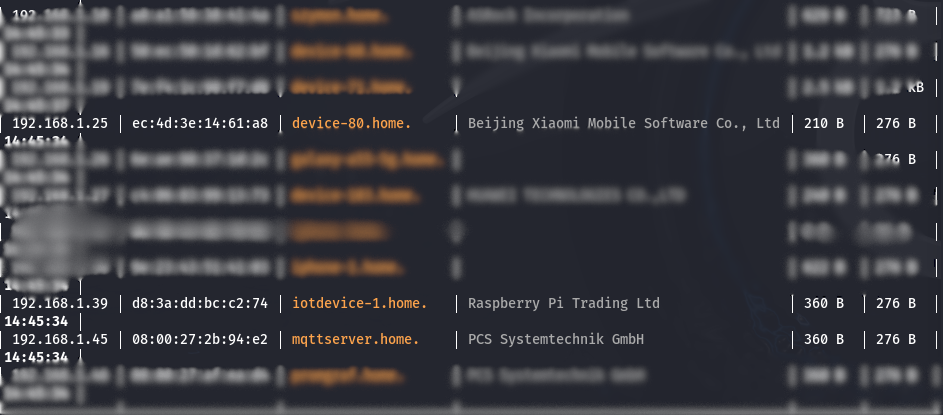
\includegraphics[width=0.8\textwidth]{pictures/net-show.png}
    \caption{Wyświetlenie listy urządzeń, przy użyciu Bettercap}
    \label{fig:Wyświetlenie listy urządzeń, przy użyciu Bettercap}
\end{figure}

W obu przypadkach atak polegał na wysyłaniu fałszywych odpowiedzi ARP, aby przekierować ruch ofiary przez system atakującego: \textit{set arp.spoof.targets 192.168.1.25 192.168.1.39}. W efekcie Kali Linux stał się pośrednikiem między urządzeniami a Routerem, wszystkie pakiety przesyłane przez ofiarę były przekierowywane.

\subsubsection{Sniffing ruchu sieciowego}
Po skutecznym przeprowadzeniu ataku ARP Spoofing, w którym ruch pomiędzy urządzeniami IoT (Raspberry Pi, poidło Xiaomi) a routerem został przekierowany przez system atakującego (Kali Linux), przystąpiono do przechwytywania i analizy danych. Wykorzystano narzędzia pasywne i aktywne w celu zbadania zawartości początkowo nieszyfrowanych komunikatów przesyłanych protokołami MQTT. 
W pierwszym etapie, za pomocą Wiresharka przechwycono nieszyfrowane komunikaty MQTT, identyfikując m.in dane przesyłane do brokera MQTT. Potwierdzono wyciek danych oraz niską odporność na wyciek danych.
Po pierwszej próbie, wdrożono zabezpieczenia przy użyciu protokołu TLS, po czym ponownie wykonano całą procedurę.

\subsubsection{Brute-force haseł}
Głównym celem przeprowadzonych testów była ocena skuteczności mechanizmów ochronnych urządzeń IoT oraz infrastruktury z nią bezpośrednio powiązanej, przed zautomatyzowanymi atakami słownikowymi. Badania obejmowały: analizę podatności na ataki brute force oraz weryfikację reakcji systemowych na wielokrotne próby logowania.
Testy przeprowadzono w kontrolowanym środowisku laboratoryjnym, z przygotowaną wcześniej infrastrukturą testową, w której aktywowano usługę SSH oraz MQTT z uwierzytelnieniem, tworząc przy tym testowe konto ze słabym hasłem. Następnie przygotowano dużą bazę haseł w formacie \textit{.txt}.
Najpierw przeprowadzono atak na protokół SSH, wykorzystując narzędzie Hydra i polecenia: \textit{hydra -l szymo -P passwordlist.txt 192.168.1.40 ssh -t 4 -vV -I}. Następnie przeprowadzano atak brute-force na broker MQTT. 

\subsubsection{Ataki DDoS}
W ramach badań przeprowadzono serię kontrolowanych ataków na środowisko testowe, w którym wyłączone zostały dodatkowe, nieistotne usługi w celu eliminacji zakłóceń. 
W pierwszym przypadku przeprowadzono atak na niezabezpieczony protokołem TLS broker MQTT, który nie wymagał uwierzytelnienia. Przy użyciu biblioteki \textit{paho.mqtt.client}, która jest bezpośrednią biblioteką do komunikacji z brokerem MQTT, stworzono skrypt w Pythonie.
\begin{lstlisting}[caption=Skrypt w Pythonie, label=lst:sensor]
    import paho.mqtt.client as mqtt
    import time
    
    broker = "192.168.1.45"
    port = 1883
    
    def flood_mqtt():
        while True:
            client = mqtt.Client()
            client.connect(broker, port)
            client.publish("test/flood", "Atak DDoS" * 1000)
            time.sleep(0.1)
    
    flood_mqtt()
\end{lstlisting}
W skrypcie przypisano adres IP brokera MQTT oraz port, na którym działa. Następnie w funkcji \textit{flood\_mqtt()} utworzono pętlę, która łączy się z brokerem i wysyła wiadomości na temat \textit{test/flood} co 0.1 sekundy. W ten sposób generowano dużą ilość ruchu, co prowadziło do przeciążenia brokera.
Podczas badania monitorowano parametry systemowe brokera MQTT.

W następnym przypadku przeprowadzono atak DDoS i DoS na protokół MQTT. Kluczowym elementem było użycie narzędzia hping3, a dokładnie polecenia: \textit{hping3 -S --flood -p 1883 192.168.1.45} w przypadku ataku z jednego adresu IP źródłowego oraz ataku rozproszonego, czyli przez zastosowanie \textit{--rand-source}. Jest to atak typu SYN Flood na port 1883 (port MQTT), wykorzystujący mechanizm nawiązywania połączeń TCP (tzw. three-way-handshake). Atakujący wysyła masowo pakiety SYN (żąda połączenia), serwer odpowiada pakietem SYN-ACK i rezerwuje zasoby (oczekuje ACK), natomiast atakujący nie wysyła ACK i pozostawia połączenie w stanie pół-otwartym.

Następnie przeprowadzono w identyczny sposób atak na protokoły UDP/55, UDP/123, TCP/22.

Na końcu przygotowano stronę HTTP, aby poddać ją ataku, przy użyciu narzędzia GoldenEye. Jest to narzędzie do przeprowadzania ataków DDoS warstwy aplikacji (HTTP Flood), które przeciąża cel poprzez masowe wysyłanie żądań HTTP. Jest napisane w Pythonie i działa na zasadzie generowania wielu równoległych połączeń, symulując ruch od wielu użytkowników. Wykonano polecenie \textit{python3 goldeneye.py http://192.168.1.45}, które: wysyła ogromną liczbę żądań HTTP (GET/POST), utrzymuje otwarte połączenia oraz używa losowych ścieżek URL. Narzędzie działa wielowątkowo, co pozwala na efektywne wykorzystanie zasobów atakującego. Wynik przechwycenia pakietów podczas tego ataku za pomocą narzędzia Wireshark przedstawia Rysunek \ref{fig:Przechwycone pakiety z programu Wireshark podczas ataku GoldenEye}.
\begin{figure}[h]
    \centering
    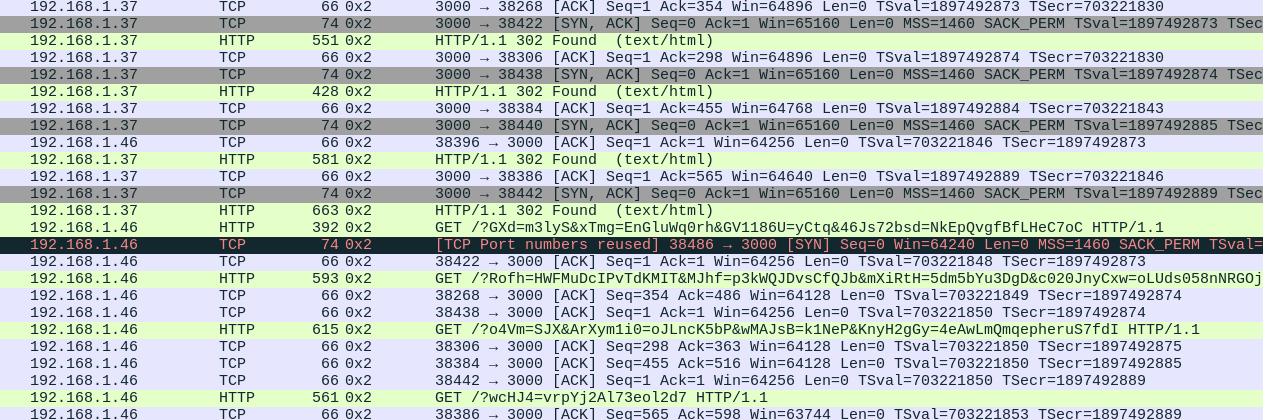
\includegraphics[width=0.8\textwidth]{pictures/wireshark-goldeneye.png}
    \caption{Przechwycone pakiety z programu Wireshark podczas ataku GoldenEye}
    \label{fig:Przechwycone pakiety z programu Wireshark podczas ataku GoldenEye}
\end{figure}

\subsection{Narzędzia wykorzystywane do testowania}
Narzędzia, które zostały wykorzystane w każdym scenariuszu i pozostawały niezmienne to:
\begin{itemize}
    \item \textbf{Infrastruktury sieciowej}: Router Wi-Fi, switch
    \item \textbf{System monitorujący:} Prometheus + Grafana na serwerze Ubuntu
\end{itemize}

\subsubsection{ARP Spoofing przy użyciu Bettercap}
Testy przeprowadzono w kontrolowanym środowisku laboratoryjnym, składającym się z:
\begin{itemize}
    \item \textbf{Urządzenia IoT:} Raspberry Pi 4B, pełniącego rolę urządzenia IoT, Xiaomi Pet Fountain
    \item \textbf{Stanowiska atakującego: } Laptop z Kali Linux (narzędzia: Bettercap, Metasploit, Wireshark, Nmap) 
\end{itemize}

\subsubsection{Sniffing ruchu sieciowego}
Testy przeprowadzono w prawie tym samym środowisku laboratoryjnym, co opisano w poprzednim scenariuszu (wykorzystując m.in. Raspberry Pi 4B oraz infrastrukturę sieciową). Do przechwycenia i analizy danych użyto narzędzi dostępnych na stanowisku atakującego (Kali Linux), w szczególności:
\begin{itemize}
    \item \textbf{Bettercap} - główna platforma do przeprowadzenia ataku ARP Spoofing oraz pasywnego sniffingu ruchu (moduły \textit{arp.spoof}, \textit{net.sniff}).
    \item \textbf{Wireshark} - narzędzie do analizy przechwyconych pakietów, umożliwiające wizualizację i dekodowanie różnych protokołów MQTT.
    \item \textbf{Nmap} - Dodatkowe skanowanie portów w celu weryfikacji aktywnych usług na urządzeniu IoT.
\end{itemize}

\subsubsection{Brute-force haseł}
Testy bezpieczeństwa przeprowadzono zgodnie z podejściem etycznego hakowania (ethical hacking), z wykorzystaniem następujących narzędzi:
\begin{itemize}
    \item \textbf{Urządzenia docelowe} - Raspberry Pi 4B, działające jako urządzenie IoT oraz Broker MQTT
    \item \textbf{Stacja atakująca} - Kali linux z narzędziami: Hydra, mqtt-pwn.
    \item \textbf{Słownik haseł} - Plik tekstowy z hasłami, zawierający 1000000 popularnych haseł, w tym domyślne hasła dla SSH i MQTT. 
\end{itemize}

\subsubsection{Ataki DDoS}
Testy przeprowadzono w kontrolowanym środowisku laboratoryjnym, składającym się z:
\begin{itemize}
    \item \textbf{Urządzenia docelowego} - Raspberry Pi 4 oraz broker MQTT Mosquitto.
    \item \textbf{Komputera atakującego} - Kali Linux z zainstalowanym Hping3, GoldenEye.
    \item \textbf{Python} - Język programowania.
    \item \textbf{Paho MQTT, time} - Biblioteka do komunikacji z brokerem MQTT, wykorzystywana do przeprowadzania ataków DoS.
\end{itemize}

\section{Ocena skuteczności zabezpieczeń IoT}
\subsection{Odporność na próby ataków}
\subsubsection{ARP Spoofing przy użyciu Bettercap}
Atak ARP spoofing został przeprowadzony w celu przejęcia kontroli nad komunikacją pomiędzy urządzeniem Xiaomi a routerem w sieci lokalnej. Urządzenie Xiaomi nie wykryło manipulacji w tablicy ARP, co potwierdziło brak mechanizmów obronnych na poziomie warstwy drugiej (L2). W urządzeniu nie zaimplementowano metod weryfikacji spójności tablic ARP, takich jak Secure ARP (S-ARP).

W kolejnym etapie badań przeprowadzono atak typu Man-in-the-Middle (MITM) na urządzenie Raspberry Pi, który zakończył się powodzeniem. Badane urządzenie komunikowało się wyłącznie z lokalnym serwerem Mosquitto MQTT, co ograniczyło możliwość wystąpienia wyraźnych anomalii w ruchu sieciowym. W przechwyconych pakietach zidentyfikowano jedynie podstawowe protokoły sieciowe, takie jak:
\begin{enumerate}
    \item \textbf{ICMP (Internet Control Message Protocol)} – wykorzystywany do diagnostyki połączeń sieciowych (np. polecenia ping),
    \item \textbf{NBNS (NetBIOS Name Service)} – protokół rozpoznawania nazw hostów w sieciach lokalnych,
    \item \textbf{MQTT} – protokół komunikacji wykorzystywany przez urządzenia IoT.
\end{enumerate}

Wykrycie ataku MITM na wczesnym etapie stanowi wyzwanie, ponieważ tego typu działania zwykle nie generują jednoznacznych sygnałów w standardowym ruchu sieciowym. W badaniach zastosowano metodę detekcji opartą na monitorowaniu dynamicznych zmian w tablicy ARP. W tym celu użyto narzędzia \textit{watch -n 1 "ip neigh show"}, umożliwiającego porównanie stanu tablicy ARP przed i po przeprowadzeniu ataku.

Analiza wykazała anomalię polegającą na obecności podwójnego wpisu dla tego samego adresu IP, lecz z różnymi adresami MAC. Jeden z wpisów wskazywał na hosta atakującego, drugi natomiast na rzeczywisty router. Zjawisko to stanowi charakterystyczny objaw ataku ARP spoofing, będącego podstawą wielu technik MITM. Efekt zaobserwowanego ataku przedstawiono na rysunku \ref{fig:Porównanie tablicy arp na urządzeniu Raspberry Pi, przed i po ataku}.
\begin{figure}[h]
    \centering
    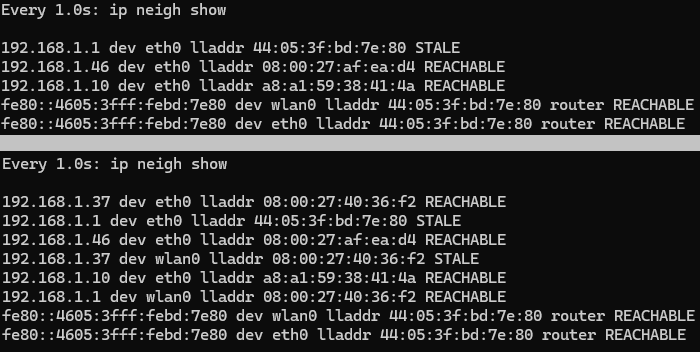
\includegraphics[width=0.8\textwidth]{pictures/arp-mitm.png}
    \caption{Porównanie tablicy ARP na urządzeniu Raspberry Pi, przed i po ataku}
    \label{fig:Porównanie tablicy arp na urządzeniu Raspberry Pi, przed i po ataku}
\end{figure}

Protokół ICMP, mimo że jest powszechnie wykorzystywany do diagnostyki, bywa również używany przez atakujących do rozpoznawania topologii sieci. Z kolei protokół NBNS, mimo swojego starszego charakteru, może ujawniać informacje dotyczące struktury sieci lokalnej, dlatego jego obecność w ruchu sieciowym ma znaczenie w kontekście bezpieczeństwa.

Zastosowana metoda detekcji, oparta na pasywnym monitorowaniu tablicy ARP, okazała się efektywna w środowisku lokalnym, w którym ruch sieciowy był ograniczony głównie do komunikacji MQTT. Automatyzacja tego procesu umożliwia szybkie wykrywanie ataków tego typu.

Testy potwierdziły, że wdrożone mechanizmy zabezpieczające, polegające na monitorowaniu i przeciwdziałaniu atakom ARP spoofing, nie wpływały negatywnie na czas reakcji urządzeń ani stabilność połączeń sieciowych. Rozwiązania te opierały się na pasywnym monitorowaniu tablicy ARP oraz stosowaniu statycznych wpisów dla krytycznych urządzeń (np. bramy domyślnej), co nie powodowało dodatkowego obciążenia procesora ani opóźnień transmisji.

Protokół ARP, pomimo swojej prostoty, działa na warstwie drugiej modelu OSI, a jego operacje realizowane są przez stos sieciowy systemu operacyjnego bez znaczącego udziału głównych zasobów obliczeniowych. W szczególności:
\begin{itemize}
    \item \textbf{Czas reakcji urządzenia} – nie przekraczał 1 ms, co jest zgodne z oczekiwaniami dla operacji ARP,
    \item \textbf{Stabilność połączeń} – nie odnotowano przerw w komunikacji ani utraty pakietów, co potwierdziło skuteczność zastosowanych zabezpieczeń.
\end{itemize}

Ponadto implementacja mechanizmów zabezpieczających przed atakami MITM nie wpłynęła w zauważalny sposób na zużycie energii ani zasobów systemowych urządzenia Raspberry Pi. Monitorowanie parametrów pracy wykazało:
\begin{itemize}
    \item \textbf{Zużycie procesora} – wzrosło nieznacznie z 0,5\% do 0,6\%,
    \item \textbf{Profil temperaturowy} – utrzymywał się średnio na poziomie 41,87 °C, co potwierdza brak dodatkowego obciążenia termicznego,
    \item \textbf{Zużycie pamięci RAM} – nie przekraczało 20 MiB, co mieści się w akceptowalnym zakresie dla operacji związanych z monitorowaniem tablicy ARP.
\end{itemize}

Podsumowując, przeciwdziałanie atakom ARP spoofing na poziomie stosu sieciowego stanowi operację o niskim koszcie obliczeniowym i nie wpływa negatywnie na wydajność systemu. W przypadku bardziej złożonych ataków, takich jak połączenie ARP spoofing z innymi technikami MITM, konieczne może być zastosowanie bardziej zaawansowanych mechanizmów obronnych, które zostaną uwzględnione w dalszych scenariuszach testowych.

\subsubsection{Sniffing ruchu sieciowego}
W trakcie przeprowadzonych testów penetracyjnych stwierdzono, że badane urządzenie Xiaomi wymienia pakiety UDP z zewnętrznym serwerem chmurowym o adresie 20.33.1.228 (należącym do infrastruktury Microsoft Azure). Wynik przechwycenia tych pakietów przedstawiono na rysunku \ref{fig:Pakiety w programie Wireshark przechwycone z urządzenia Xiaomi}.
\begin{figure}[h]
    \centering
    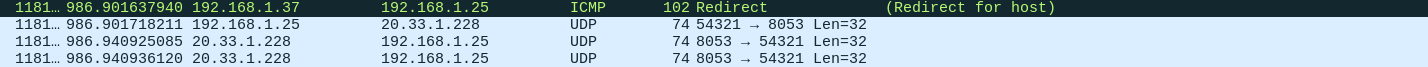
\includegraphics[width=0.8\textwidth]{pictures/wireshark-mitm-xiaomi.png}
    \caption{Pakiety w programie Wireshark przechwycone z urządzenia Xiaomi}
    \label{fig:Pakiety w programie Wireshark przechwycone z urządzenia Xiaomi}
\end{figure}

Analiza ruchu sieciowego wykazała następujące charakterystyki bezpieczeństwa:

\textbf{Brak zabezpieczeń na warstwie sieciowej:}  
Przechwycone pakiety nie zawierały nagłówków kryptograficznych ani mechanizmów uwierzytelniania protokołu UDP.

\textbf{Charakterystyka szyfrowania:}  
Urządzenie stosowało szyfrowanie lokalne z kluczem symetrycznym (np. AES-256) zapisanym w pamięci firmware, co potwierdzała stała długość (32 bajty) i struktura zaszyfrowanego payloadu. Wdrożony został model hybrydowy z deszyfracją w chmurze, w którym serwer odbierał dane w postaci struktury binarnej i deszyfrował je przy użyciu dedykowanego klucza, prawdopodobnie z wykorzystaniem klucza sesyjnego wyprowadzanego z unikalnego identyfikatora urządzenia.

\textbf{Minimalistyczna architektura sieciowa:}  
Wyniki skanowania portów (nmap -sS/-sU) potwierdziły, że urządzenie:
\begin{itemize}
    \item nie udostępniało żadnych usług sieciowych (TCP/UDP) poza komunikacją wychodzącą na porcie 8053/UDP,
    \item działało w modelu \textit{„fire-and-forget”}, tj. inicjowało wyłącznie połączenia do chmury,
    \item implementowało zasadę \textit{zero trust} dla połączeń przychodzących.
\end{itemize}

\textbf{Zidentyfikowane zagrożenia:}  
Pomimo braku otwartych portów urządzenie pozostawało podatne na:
\begin{itemize}
    \item ataki MITM poprzez ARP spoofing, umożliwiające przechwycenie danych w tranzycie,
    \item analizę statystyczną zaszyfrowanych pakietów, mogącą prowadzić do złamania klucza przy długotrwałym przechwytywaniu ruchu,
    \item ataki na fizyczne zabezpieczenia urządzenia, w tym potencjalną ekstrakcję klucza z pamięci firmware.
\end{itemize}

Przeanalizowany protokół komunikacyjny wykazywał cechy typowe dla rozwiązań IoT klasy konsumenckiej, w których priorytetem jest minimalizacja zużycia energii kosztem pełnej transparentności kryptograficznej. Brak implementacji mechanizmów zabezpieczeń warstwy transportowej stanowi istotne ograniczenie w kontekście środowisk o podwyższonym poziomie ryzyka.

W przypadku urządzenia Raspberry Pi stwierdzono dodatkowe luki bezpieczeństwa w komunikacji MQTT. Przechwycone pakiety ujawniły następujące problemy, zobrazowane na rysunku \ref{fig:Pakiety w programie Wireshark przechwycone z urządzenia Raspberry Pi}.
\begin{figure}[h]
    \centering
    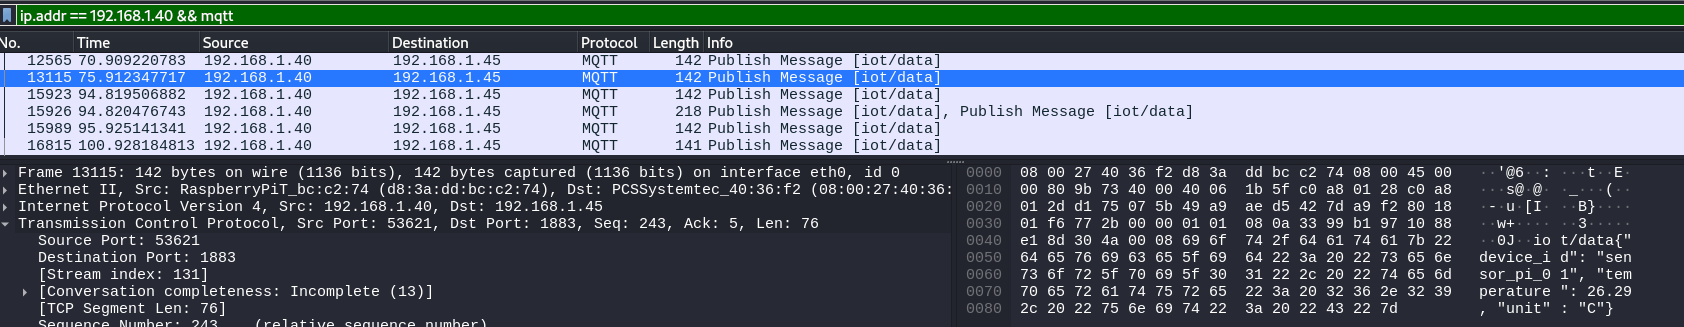
\includegraphics[width=0.8\textwidth]{pictures/sniffwireshark.png}
    \caption{Pakiety w programie Wireshark przechwycone z urządzenia Raspberry Pi}
    \label{fig:Pakiety w programie Wireshark przechwycone z urządzenia Raspberry Pi}
\end{figure}

\textbf{Dane przesyłane jawnym tekstem:}  
Pełna treść wiadomości MQTT była dostępna w formie niezaszyfrowanego JSON:
\begin{verbatim}
{
"device_id": "sensor_pi_01",
"temperature": 26.29,
"unit": "C"
}
\end{verbatim}
Brakowało mechanizmów szyfrowania na poziomie transportowym (TLS) i aplikacyjnym.

\textbf{Brak mechanizmów uwierzytelniania:}  
Broker MQTT nie wymagał uwierzytelnienia klienta ani nie stosował weryfikacji autentyczności wiadomości.

\textbf{Niski poziom QoS:}  
Wykorzystywano QoS 0 (\textit{„fire-and-forget”}), co zwiększało ryzyko utraty danych, a jednocześnie brakowało potwierdzenia doręczenia wiadomości.

\textbf{Przewidywalna struktura komunikacji:}  
Stały temat (topic) „iot/data” ułatwiał identyfikację strumieni danych, a regularny format JSON umożliwiał łatwą interpretację przechwyconych informacji.

W odróżnieniu od urządzenia Xiaomi, w którym zastosowano szyfrowanie lokalne, analizowany broker MQTT nie implementował żadnych mechanizmów zabezpieczających. Stanowiło to poważne zagrożenie w kontekście przesyłania danych sensorycznych, które mogą zawierać informacje o monitorowanym środowisku.

W kolejnym scenariuszu wdrożono protokół TLS, zapewniający szyfrowanie komunikacji między urządzeniem IoT a brokerem MQTT. Wykorzystano certyfikaty X.509 do uwierzytelnienia serwera oraz klienta, co istotnie zwiększyło bezpieczeństwo transmisji. Dane aplikacyjne, wcześniej dostępne w postaci jawnego tekstu, zostały po implementacji TLS przesyłane jako zaszyfrowany strumień bajtów. Komunikacja została przeniesiona na port 8883 (MQTTS), a każda sesja rozpoczynała się od pełnego handshake'a TLS. Broker wymagał przedstawienia ważnego certyfikatu klienta podpisanego przez zaufany urząd certyfikacji (CA).

Wdrożenie protokołu TLS podniosło poziom bezpieczeństwa systemu przy zachowaniu akceptowalnego zużycia zasobów obliczeniowych. Jak przedstawiono na rysunku \ref{fig:Wykresy monitorujące Raspberry Pi w trakcie wdrażania TLS, przy pomocy Grafany}, analiza metryk wydajnościowych urządzenia wykazała:
\begin{itemize}
    \item \textbf{Obciążenie procesora} – w stanie bazowym (przed implementacją TLS) na poziomie ok. 1\%; podczas inicjalizacji TLS (21:05) wzrost do 24\% i powrót do wartości bazowych w czasie poniżej 5 minut,
    \item \textbf{Pobór mocy} – brak zauważalnych zmian,
    \item \textbf{Zużycie pamięci RAM} – wzrost o ok. 50 MiB podczas inicjalizacji TLS i stabilizacja na nowym poziomie z marginesem poniżej 5\% względem wartości początkowej.
\end{itemize}

\begin{figure}[h]
    \centering
    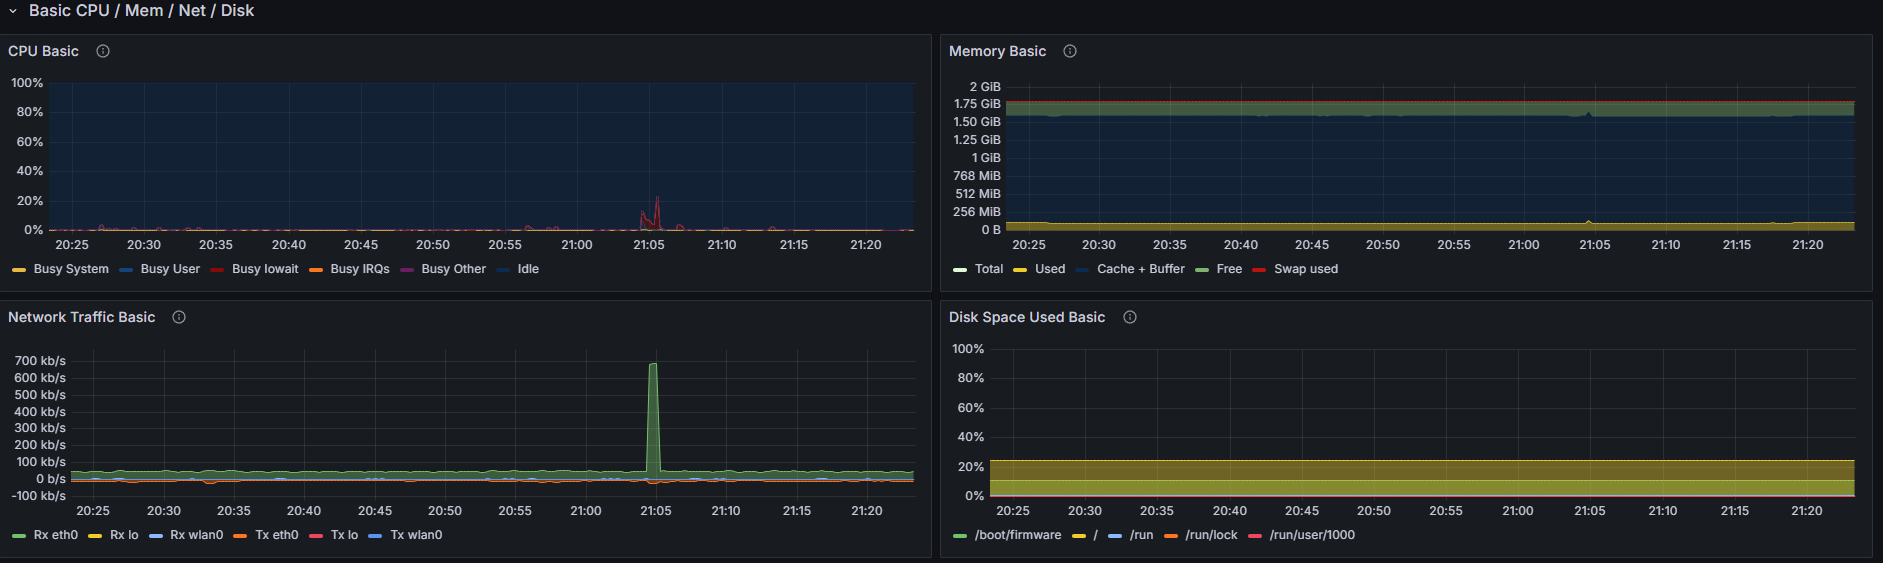
\includegraphics[width=0.8\textwidth]{pictures/raspberry-tls.png}
    \caption{Wykresy monitorujące Raspberry Pi w trakcie wdrażania TLS, przy pomocy Grafany} 
    \label{fig:Wykresy monitorujące Raspberry Pi w trakcie wdrażania TLS, przy pomocy Grafany}
\end{figure}

Uzyskane wyniki potwierdzają, że koszt wydajnościowy wprowadzenia szyfrowania TLS pozostaje niewielki w stosunku do uzyskanych korzyści w zakresie bezpieczeństwa. Tymczasowy wzrost zużycia zasobów podczas inicjalizacji połączenia (tzw. koszt handshake'a TLS) miał charakter incydentalny i nie wpływał na stabilność systemu. W środowiskach IoT, w których dane są przesyłane w interwałach dłuższych niż 5 s, zaobserwowany wzrost zużycia zasobów należy ocenić jako:
\begin{itemize}
    \item \textbf{akceptowalny} – zgodnie z normą ISO/IEC 27001 dla systemów klasy II,
    \item \textbf{proporcjonalny} – do uzyskanej ochrony przed sniffingiem i atakami MITM,
    \item \textbf{kompatybilny} – z wymaganiami dla systemów IoT, w których priorytetem jest minimalizacja zużycia energii.
\end{itemize}

Podsumowanie różnic w poziomie bezpieczeństwa przedstawiono w tabeli \ref{tab:security_comparison}.
\begin{table}[h]
    \centering
    \caption{Porównanie właściwości bezpieczeństwa komunikacji MQTT z uwzględnieniem implementacji TLS}
    \label{tab:security_comparison}
    \begin{tabular}{|l|c|c|}
        \hline
        \textbf{Parametr bezpieczeństwa} & \textbf{Bez TLS} & \textbf{Z TLS} \\ \hline
        Poufność danych & Nie & Tak \\ \hline
        Integralność danych & Nie & Tak \\ \hline
        Uwierzytelnienie & Nie & Tak \\ \hline
        Ochrona przed wyciekiem danych & Nie & Tak \\ \hline
    \end{tabular}
\end{table}

\subsubsection{Brute-force haseł}
Przeprowadzone testy ataków brute force na protokoły SSH i MQTT umożliwiły ocenę odporności badanych urządzeń IoT na próby nieautoryzowanego dostępu. W przypadku protokołu SSH stwierdzono, że:
\begin{enumerate}
    \item Standardowa konfiguracja usługi SSH (bez dodatkowych zabezpieczeń) umożliwiała złamanie słabego hasła (6-znakowego, bez znaków specjalnych) w czasie średnio 4 minut przy użyciu narzędzia Hydra z słownikiem 100000 najpopularniejszych haseł.
    \item Włączenie modułu fail2ban (blokada po 3 nieudanych próbach) całkowicie uniemożliwiało atak brute force.
\end{enumerate}

Dla protokołu MQTT uzyskane wyniki wskazały, że:
\begin{enumerate}
    \item Broker Mosquitto bez dodatkowej konfiguracji był podatny na ataki słownikowe.
    \item Aktywacja blokady po 5 nieudanych próbach oraz wymóg stosowania certyfikatów TLS znacząco poprawiały poziom bezpieczeństwa.
\end{enumerate}

Wyniki prób ataku przedstawiono na rysunku \ref{fig:Porównanie próby złamania hasła na Raspberry Pi, przy użyciu narzędzia Hydra przed i po zabezpieczeniu}. W pierwszym przypadku, bez dodatkowych zabezpieczeń, atak zakończył się powodzeniem w ciągu kilku minut. Po wdrożeniu mechanizmu fail2ban oraz silnych haseł próba ataku nie powiodła się, a narzędzie Hydra nie było w stanie znaleźć poprawnego hasła w czasie dłuższym niż 24 godziny.
\begin{figure}[h]
    \centering
    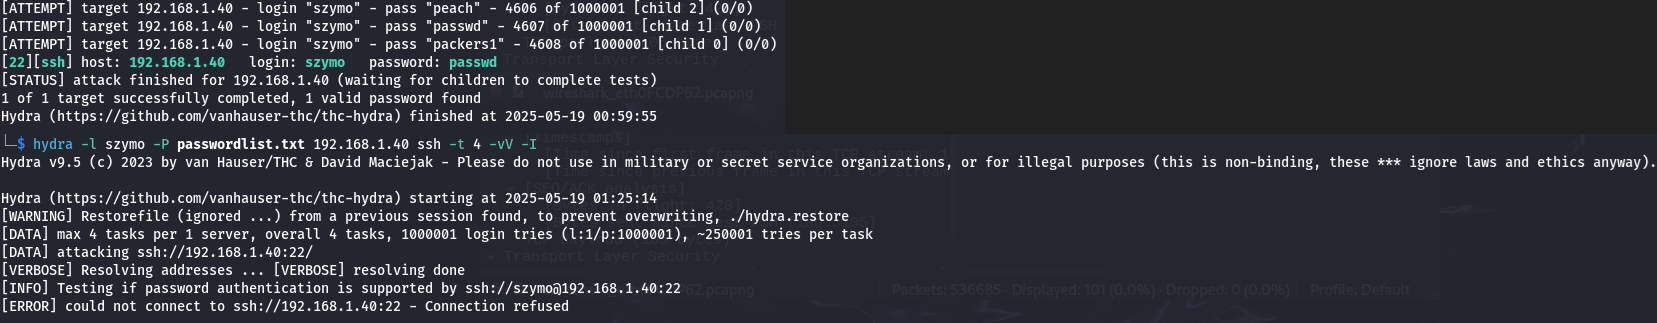
\includegraphics[width=0.8\textwidth]{pictures/hydra-atack-pi.png}
    \caption{Porównanie próby złamania hasła na Raspberry Pi, przy użyciu narzędzia Hydra przed i po zabezpieczeniu}
    \label{fig:Porównanie próby złamania hasła na Raspberry Pi, przy użyciu narzędzia Hydra przed i po zabezpieczeniu}
\end{figure}

Przeprowadzone badania wykazały, że jednym z najskuteczniejszych oraz najmniej obciążających system rozwiązań jest stosowanie silnych haseł w połączeniu z podstawowymi mechanizmami ochronnymi. W przeciwieństwie do zaawansowanych mechanizmów kryptograficznych, które mogą znacząco obciążać procesor i pamięć, stosowanie odpowiednio skonstruowanych haseł nie powodowało zauważalnego wpływu na:
\begin{itemize}
    \item zużycie energii elektrycznej,
    \item stabilność połączeń,
    \item czas reakcji urządzenia,
    \item obciążenie procesora,
    \item zużycie pamięci RAM.
\end{itemize}

Na rysunku \ref{fig:Wykresy monitorujące Raspberry Pi w trakcie ataku Brute Force, przy pomocy Grafany} przedstawiono wyniki monitorowania urządzenia podczas ataku brute force. Zaobserwowano wzrost wykorzystania CPU o 9,2\% ±0,5\% w stosunku do stanu spoczynkowego. W przypadku ataku trwającego dłuższy czas temperatura procesora wzrosła o około 5 °C, co może wpływać na funkcjonowanie urządzenia.
\begin{figure}[h]
    \centering
    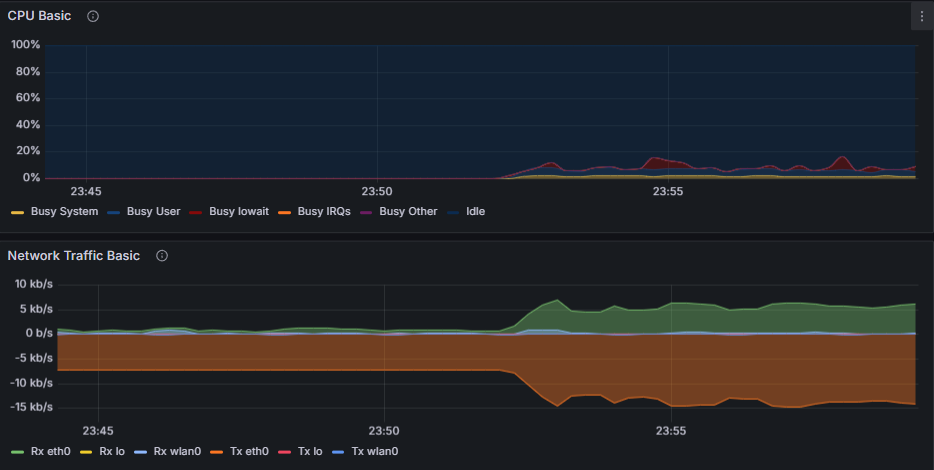
\includegraphics[width=0.8\textwidth]{pictures/brute-force-pi.png}
    \caption{Wykresy monitorujące Raspberry Pi w trakcie ataku Brute Force, przy pomocy Grafany}
    \label{fig:Wykresy monitorujące Raspberry Pi w trakcie ataku Brute Force, przy pomocy Grafany}
\end{figure}

Uzyskane wyniki potwierdziły, że to sam proces ataku, a nie wdrożone mechanizmy ochronne, stanowił główne źródło obciążenia systemu. Wykres wskazuje na korelację między intensywnością ataku a wzrostem wykorzystania zasobów. Mechanizmy takie jak fail2ban pełnią istotną rolę w minimalizacji wpływu ataków poprzez wczesne wykrywanie charakterystycznych wzorców i automatyczną blokadę źródłowych adresów IP. Dane empiryczne wykazały, że prawidłowo skonfigurowany fail2ban (parametry: bantime=1h, findtime=10m, maxretry=3) pozwalał na ograniczenie obciążenia procesora oraz skrócenie czasu powrotu do stanu nominalnego. Wyniki te potwierdziły zasadność stosowania lekkich mechanizmów ochronnych na urządzeniach IoT, które skutecznie redukują negatywny wpływ ataków bez generowania znaczącego obciążenia systemu.

Dodatkowo stwierdzono, że zastosowanie słabych haseł stanowi czynnik krytyczny w skuteczności ataków brute force. Zastosowanie haseł spełniających dobre praktyki bezpieczeństwa znacząco wydłuża czas potrzebny do ich złamania. Szacunkowe obliczenia wskazują, że dla współczesnych mocy obliczeniowych czas ten może wynosić setki lat, przy czym rozwiązanie to pozostaje neutralne dla wydajności systemu.

\subsubsection{Ataki DDoS}
Ataki typu DDoS (Distributed Denial of Service) na urządzenia IoT stanowią jedno z najpoważniejszych i najczęściej spotykanych zagrożeń we współczesnych systemach sieciowych. Celem ich przeprowadzenia jest zazwyczaj przeciążenie zasobów urządzenia lub usługi, co prowadzi do braku dostępności kluczowych funkcjonalności.

W pierwszym etapie badań atak został skierowany na brokera MQTT działającego bez mechanizmów uwierzytelniania. Za pomocą skryptu w języku Python wykonano próbę ataku DoS na lokalny serwer Mosquitto. Choć obserwowano niewielki wzrost obciążenia CPU wraz ze wzrostem częstotliwości przesyłania pakietów, nie wpłynęło to w istotny sposób na stabilność połączenia ani dostępność usługi. Zauważono jednak, że atak tego typu może pełnić inny cel — masowe przesyłanie danych typu „Atak DoS” do brokera MQTT mogłoby doprowadzić do zapełnienia bazy danych i utrudnienia analizy rzeczywistych komunikatów.

W momencie, gdy komunikacja została zabezpieczona protokołem TLS wraz z certyfikatami klienta, atak zakończył się całkowitym niepowodzeniem. Broker MQTT skutecznie odrzucał wszystkie połączenia, dla których certyfikaty nie mogły zostać zweryfikowane.

\medskip
W kolejnym etapie zastosowano narzędzie \textit{hping3}, umożliwiające przeprowadzenie złożonych ataków DDoS. Wyniki przedstawiono na rysunku \ref{fig:Wykresy moniturujące broker MQTT w trakcie ataku DDOS, przy pomocy Grafany1}. 
\begin{enumerate}
    \item \textbf{Atak z losowymi, fałszowanymi adresami IP} – doprowadził do skokowego wzrostu obciążenia CPU do 100\% oraz podniesienia temperatury procesora do 80°C. Broker MQTT przestał odpowiadać na zapytania, co jednoznacznie potwierdziło skuteczność ataku. Mimo to możliwe było wykonywanie zapytań do zewnętrznych serwisów (np. www.wp.pl), choć z dużym opóźnieniem (328 ms).
    \item \textbf{Atak z jednego źródła IP} – spowodował wzrost obciążenia CPU do około 60\%. Broker MQTT nadal działał, jednak opóźnienia odpowiedzi wzrosły do około 220 ms. Test potwierdził, że pojedynczy atak jest mniej efektywny niż skoordynowany ruch z wielu źródeł.
\end{enumerate}

\begin{figure}[h]
    \centering
    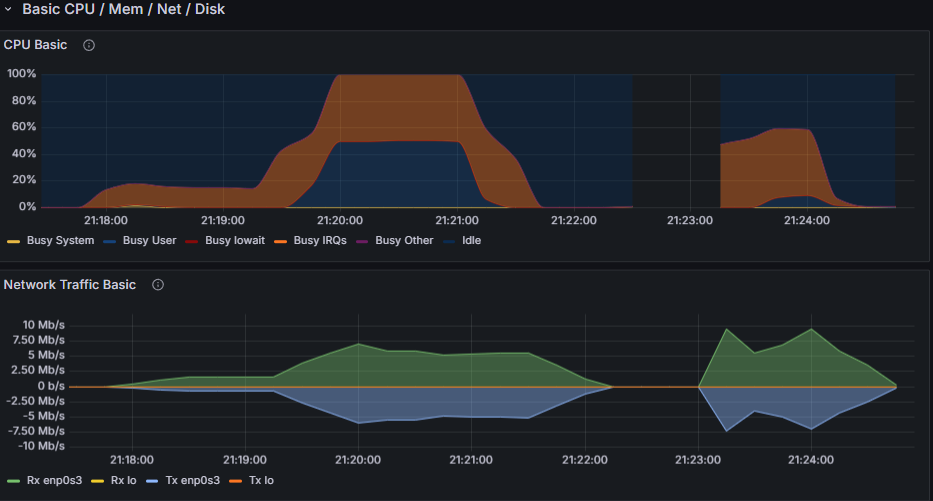
\includegraphics[width=0.8\textwidth]{pictures/hping-mqtt-z -i-bez.png}
    \caption{Wykresy monitorujące broker MQTT w trakcie ataku DDoS, przy pomocy Grafany}
    \label{fig:Wykresy moniturujące broker MQTT w trakcie ataku DDOS, przy pomocy Grafany1}
\end{figure}

W dalszych eksperymentach przeprowadzono ataki DDoS skierowane na protokoły UDP/53, UDP/123 oraz TCP/22, co przedstawiono na rysunku \ref{fig:Wykresy moniturujące broker MQTT w trakcie ataku DDOS na różne protokoły, przy pomocy Grafany2}. Obserwowano wzrost średniego obciążenia procesora do około 50\%. Po zakończeniu ataku broker powracał do stabilnej pracy. Ataki te okazały się mniej skuteczne niż te wymierzone bezpośrednio w port MQTT, co podkreśla znaczenie właściwej ochrony kluczowych usług sieciowych.

\begin{figure}[h]
    \centering
    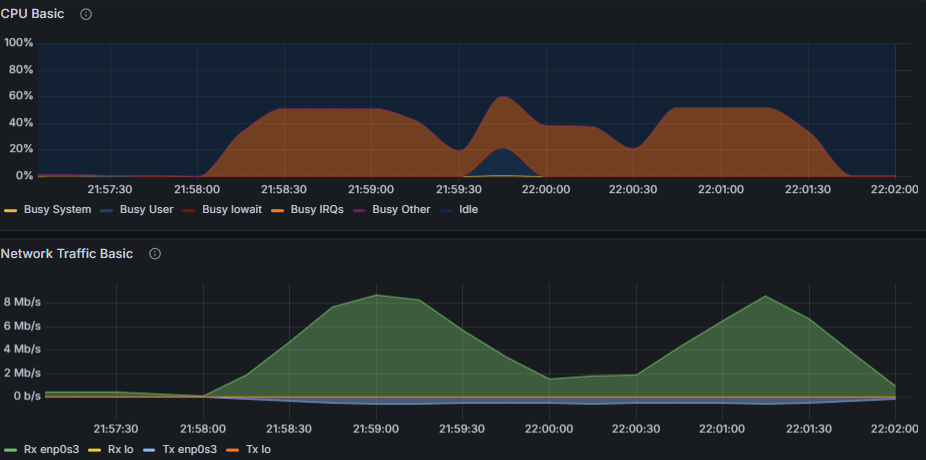
\includegraphics[width=0.8\textwidth]{pictures/hping-protokoly.png}
    \caption{Wykresy monitorujące broker MQTT w trakcie ataku DDoS na różne protokoły, przy pomocy Grafany}
    \label{fig:Wykresy moniturujące broker MQTT w trakcie ataku DDOS na różne protokoły, przy pomocy Grafany2}
\end{figure}

Ponieważ część urządzeń IoT komunikuje się również przy użyciu protokołu HTTP, przeprowadzono test z wykorzystaniem narzędzia \textit{GoldenEye}. Atak został skierowany na serwer HTTP działający obok brokera Mosquitto. W jego wyniku obciążenie CPU wzrosło do 80\%, a usługa HTTP przestała odpowiadać już po około 10 sekundach. Po zakończeniu ataku system wrócił do nominalnej pracy. Badanie to wykazało, że ataki skierowane na warstwę aplikacyjną mogą być wyjątkowo skuteczne i trudniejsze do odparcia.

\medskip
W ramach działań ochronnych wdrożono reguły firewalla \texttt{iptables}, m.in. blokujące nieużywane porty oraz limitujące liczbę równoczesnych połączeń TCP do pięciu przy użyciu reguły:
\begin{verbatim}
sudo iptables -A INPUT -p tcp --syn -m connlimit --connlimit-above 5 -j DROP
\end{verbatim}
Dodatkowo w konfiguracji Mosquitto ustawiono limity liczby równoczesnych połączeń. Zastosowane rozwiązania znacząco zmniejszyły skuteczność ataków, a w niektórych przypadkach całkowicie je neutralizowały, bez negatywnego wpływu na stabilność i wydajność systemu.

\medskip
Podsumowując, przeprowadzone eksperymenty wykazały wysoką podatność urządzeń IoT na ataki DDoS, które w skrajnych przypadkach mogą prowadzić do całkowitej niedostępności usług. Odpowiednia konfiguracja zabezpieczeń, takich jak firewalle, systemy wykrywania intruzów oraz monitoring ruchu sieciowego, jest kluczowa dla zapewnienia odporności i ciągłości działania infrastruktury IoT.

\section{Podsumowanie testów zabezpieczeń}
Przeprowadzone w niniejszym rozdziale testy miały na celu praktyczną ocenę skuteczności zabezpieczeń systemów IoT w kontrolowanym środowisku laboratoryjnym. Zastosowano wielowarstwowe podejście do testowania, obejmujące ataki na warstwę łącza danych (ARP Spoofing), aplikacyjną (Sniffing, Brute-Force) oraz ataki typu Denial of Service.

Główne ustalenia z przeprowadzonych scenariuszy testowych przedstawia tabela \ref{tab:podsumowanie-testow}.
\begin{table}[htbp]
\centering
\caption{Podsumowanie wyników testów zabezpieczeń IoT}
\begin{tabular}{p{4.5cm} p{5cm} p{5cm}}
\toprule
\textbf{Scenariusz testowy} & \textbf{Stan początkowy (brak zabezpieczeń)} & \textbf{Stan po wdrożeniu zabezpieczeń} \\
\midrule
\textbf{ARP Spoofing / MITM} & Pełna podatność. Udane przejęcie sesji komunikacyjnych dla wszystkich testowanych urządzeń. & Wykrywanie dzięki monitorowaniu tablicy ARP. Brak negatywnego wpływu na wydajność systemu. \\
\midrule
\textbf{Sniffing ruchu} & Pełny wyciek danych (JSON w postaci jawnej). Podatność na analizę ruchu (Xiaomi). & Skuteczne zaszyfrowanie danych przy użyciu TLS. Akceptowalny, chwilowy wzrost zużycia CPU. \\
\midrule
\textbf{Brute-Force} & Hasła łamane w kilka minut. Wysokie obciążenie systemu podczas ataku. & Blokada ataków dzięki mechanizmowi fail2ban. Brak wpływu silnych haseł na wydajność systemu. \\
\midrule
\textbf{DDoS} & Całkowite przeciążenie usług (100\% CPU, brak odpowiedzi). Skuteczne ataki z wielu źródeł. & Skuteczna ochrona dzięki regułom \texttt{iptables} i limitowaniu połączeń. Przywrócona stabilność działania. \\
\bottomrule
\label{tab:podsumowanie-testow}
\end{tabular}
\end{table}

Podsumowując, testy jednoznacznie wykazały, że podstawowe, niechronione konfiguracje systemów IoT są wysoce podatne na szeroki wachlarz ataków. Jednocześnie potwierdziły one wysoką skuteczność i relatywnie niski koszt wydajnościowy wdrożenia fundamentalnych środków ochrony, takich jak:
\begin{itemize}
    \item szyfrowanie komunikacji (TLS),
    \item egzekwowanie stosowania silnych haseł oraz mechanizmów blokady (fail2ban),
    \item podstawowa filtracja ruchu sieciowego (firewall),
    \item ciągłe monitorowanie aktywności systemowej.
\end{itemize}

Wyniki te dostarczają cennych danych praktycznych dotyczących odporności systemów IoT na cyberataki i stanowią istotną podstawę do sformułowania ogólnych wniosków oraz rekomendacji końcowych, przedstawionych w dalszej części pracy.
 

\chapter{Zgodność zabezpieczeń IoT z regulacjami dotyczącymi prywatności}
\label{chap:rozdzial6}
\section{Ocena zgodności zabezpieczeń z regulacjami dotyczącymi prywatności}
Wraz z dynamicznym rozwojem Internetu Rzeczy wzrasta znaczenie ochrony danych przetwarzanych przez urządzenia podłączone do sieci. Ze względu na wrażliwość tych danych, konieczne jest zapewnienie zgodności systemów IoT z obowiązującymi regulacjami prawnymi dotyczącymi prywatności. W tym rozdziale przeanalizowano kluczowe przepisy prawne, takie jak RODO (GDPR), HIPAA oraz inne istotne regulacje, a także zbadano wymogi dotyczące ochrony danych osobowych w systemach IoT oraz oceniono poziom zgodności stosowanych zabezpieczeń z obowiązującym prawem.

\subsection{Przegląd regulacji prawnych (RODO, HIPAA, itd.)}

\subsubsection{Ogólne Rozporządzenie o Ochronie Danych (RODO/GDPR)}
RODO (Rozporządzenie Parlamentu Europejskiego i Rady (UE) 2016/679 \cite{gdpr2016}), znane także jako GDPR (General Data Protection Regulation), stanowi fundament prawny dotyczący ochrony danych osobowych w Unii Europejskiej. W kontekście Internetu Rzeczy (IoT), gdzie urządzenia zbierają, przesyłają i przetwarzają dane osobowe w sposób często zautomatyzowany i ciągły, rozporządzenie to ma kluczowe znaczenie.
\textbf{Zasada prywatności przez projekt (Privacy by Design)} - Twórcy i producenci urządzeń IoT mają obowiązek uwzględniać kwestie ochrony danych już na etapie projektowania i wdrażania urządzeń i systemów. Oznacza to m.in. konieczność:
\begin{itemize}
    \item domyślnego wyłączania zbędnych funkcji zbierania danych,
    
    \item stosowania domyślnych ustawień prywatności,
    
    \item projektowania interfejsów w sposób zrozumiały i przejrzysty dla użytkownika (tzw. privacy UX).
\end{itemize}

\textbf{Minimalizacja danych} - Zgodnie z RODO, przetwarzane mogą być tylko te dane osobowe, które są niezbędne do realizacji konkretnego celu. W kontekście IoT oznacza to:
\begin{itemize}
    \item ograniczenie liczby zbieranych parametrów (np. tylko temperatura, bez lokalizacji),
    
    \item unikanie gromadzenia danych zapasowych lub nadmiarowych,
    
    \item regularne usuwanie niepotrzebnych informacji.
\end{itemize}

\textbf{Bezpieczeństwo przetwarzania} - Administratorzy i podmioty przetwarzające dane muszą wdrożyć odpowiednie środki techniczne i organizacyjne, aby zapewnić ich bezpieczeństwo. W IoT mogą to być:
\begin{itemize}
    \item szyfrowanie transmisji (np. TLS, DTLS),
    
    \item stosowanie silnych haseł lub uwierzytelniania dwuskładnikowego (2FA),
    
    \item bezpieczne aktualizacje oprogramowania (OTA),
    
    \item fizyczne zabezpieczenia urządzeń końcowych.
\end{itemize}

\textbf{Obowiązek informacyjny} - Użytkownik końcowy musi być jasno poinformowany: 
\begin{itemize}
    \item jakie dane są zbierane (np. dane lokalizacyjne, biomedyczne),
    
    \item w jakim celu i przez kogo są przetwarzane,

    \item jak długo dane będą przechowywane,
    
    \item jakie przysługują mu prawa.
\end{itemize}
W przypadku wielu urządzeń IoT, które nie posiadają ekranów ani interfejsu użytkownika, realizacja tego obowiązku może być trudna – dlatego zalecane są np. aplikacje mobilne z rozbudowanymi politykami prywatności lub strony internetowe z informacjami.

\textbf{Prawa osób, których dane dotyczą} - RODO przyznaje osobom fizycznym szereg praw, które muszą być również respektowane w środowisku IoT:
\begin{itemize}
    \item \textbf{prawo do dostępu do danych} – użytkownik może żądać pełnej informacji o przetwarzanych danych,

    \item \textbf{prawo do sprostowania danych} – np. poprawienie błędnych danych zdrowotnych w opasce fitness,

    \item \textbf{prawo do usunięcia danych} („prawo do bycia zapomnianym”) – np. usunięcie historii lokalizacji z chmury producenta,

    \item \textbf{prawo do przenoszenia danych} – możliwość eksportu danych z jednego urządzenia/usługi do innego dostawcy,

    \item \textbf{prawo do sprzeciwu} wobec przetwarzania danych w określonym celu (np. marketingowym).
\end{itemize}


\subsubsection{Ustawa HIPAA (Health Insurance Portability and Accountability Act)}
HIPAA to amerykańska ustawa przyjęta w 1996 roku \cite{hipaa_security_rule}, która reguluje ochronę danych osobowych w sektorze opieki zdrowotnej, ze szczególnym uwzględnieniem danych medycznych i zdrowotnych pacjentów. W kontekście IoT, gdzie coraz więcej urządzeń medycznych i monitorujących zdrowie zbiera i przetwarza dane wrażliwe, HIPAA wprowadza szereg wymogów mających na celu zapewnienie ich bezpieczeństwa oraz prywatności.

\begin{itemize}
\item \textbf{Zabezpieczenia danych wrażliwych} – HIPAA wymaga stosowania odpowiednich środków technicznych i organizacyjnych, takich jak szyfrowanie danych zarówno podczas ich przesyłania (np. szyfrowanie TLS) jak i w stanie spoczynku (np. szyfrowanie na dyskach urządzeń). Ponadto konieczne jest wdrożenie kontroli dostępu (autoryzacja użytkowników, role i uprawnienia), które ograniczają dostęp tylko do osób uprawnionych. W kontekście IoT, urządzenia muszą mieć zabezpieczenia chroniące przed nieautoryzowanym dostępem oraz mechanizmy uwierzytelniania.

\item \textbf{Ograniczone udostępnianie danych} – HIPAA nakłada restrykcje dotyczące udostępniania danych osobowych i medycznych. Dane mogą być przekazywane tylko podmiotom uprawnionym (np. lekarzom, ubezpieczycielom) oraz za zgodą pacjenta, chyba że przepisy prawa stanowią inaczej. W urządzeniach IoT, które zbierają dane zdrowotne, ważne jest, aby komunikacja i wymiana danych była kontrolowana i zgodna z tymi wymogami, zapobiegając nieautoryzowanemu udostępnianiu lub sprzedaży informacji.

\item \textbf{Raportowanie naruszeń bezpieczeństwa} – HIPAA wymaga, aby organizacje, które zarządzają danymi zdrowotnymi, w przypadku naruszenia bezpieczeństwa (np. wycieku danych, ataku hakerskiego), niezwłocznie zgłaszały incydent odpowiednim organom nadzorczym oraz osobom, których dane dotyczą. Procedury te mają na celu szybkie przeciwdziałanie skutkom naruszenia, ograniczenie szkód oraz zwiększenie transparentności wobec użytkowników.

\item \textbf{Audyt i monitorowanie} – HIPAA zaleca regularne audyty bezpieczeństwa systemów przetwarzających dane zdrowotne oraz monitorowanie dostępu do danych w celu wykrywania nieprawidłowości i potencjalnych zagrożeń. W systemach IoT może to oznaczać implementację narzędzi do monitoringu ruchu sieciowego, analizy logów oraz alarmowania o nietypowych działaniach.

\item \textbf{Szkolenia personelu} – HIPAA podkreśla konieczność regularnego szkolenia pracowników i użytkowników systemów w zakresie ochrony danych i bezpieczeństwa informacji. Dotyczy to również osób obsługujących urządzenia IoT, aby minimalizować ryzyko błędów ludzkich i świadomie przestrzegać zasad bezpieczeństwa.
\end{itemize}
Ze względu na rosnącą popularność urządzeń IoT w sektorze zdrowotnym, takich jak opaski monitorujące parametry życiowe, urządzenia do telemedycyny czy inteligentne implanty, przestrzeganie wymogów HIPAA jest kluczowe dla ochrony danych pacjentów oraz zgodności z prawem.

\subsubsection{Inne regulacje dotyczące prywatności}

Oprócz RODO i HIPAA, istnieje wiele innych istotnych regulacji na świecie, które mają na celu ochronę danych osobowych i prywatności użytkowników, także w kontekście Internetu Rzeczy (IoT):

\begin{itemize}

\item \textbf{CCPA (California Consumer Privacy Act)} – to kalifornijska ustawa o ochronie danych osobowych, która daje mieszkańcom Kalifornii szereg praw dotyczących ich danych. Konsumenci mają prawo do informacji o tym, jakie dane są zbierane, w jakim celu, a także prawo do żądania ich usunięcia. Ustawa wprowadza także wymogi dotyczące przejrzystości, zabezpieczeń oraz ogranicza sprzedaż danych osobowych firmom trzecim. W kontekście IoT oznacza to konieczność jasnego informowania użytkowników urządzeń o tym, jakie informacje są zbierane i jak są wykorzystywane \cite{ccpa}.

\item \textbf{PDPA (Personal Data Protection Act)} – singapurska ustawa regulująca przetwarzanie danych osobowych. PDPA wymaga uzyskania zgody użytkownika na przetwarzanie jego danych oraz nakłada obowiązek zapewnienia odpowiednich środków technicznych i organizacyjnych chroniących te dane. W kontekście IoT reguluje to m.in. kwestie zbierania danych przez inteligentne urządzenia oraz ich bezpiecznego przechowywania \cite{pdpa}.

\item \textbf{PIPEDA (Personal Information Protection and Electronic Documents Act)} – kanadyjska ustawa dotycząca ochrony danych osobowych, która podobnie jak PDPA, wymaga zgody na przetwarzanie danych oraz stosowania odpowiednich zabezpieczeń. Wdrażanie tej ustawy w sektorze IoT wymaga od firm zapewnienia odpowiedniej polityki prywatności i bezpieczeństwa urządzeń, szczególnie w zakresie danych osobowych użytkowników \cite{pipeda}.

\item \textbf{LGPD (Lei Geral de Proteção de Dados)} – brazylijska ustawa o ochronie danych osobowych, wzorowana na RODO, wprowadzająca wymogi dotyczące zgody na przetwarzanie danych, minimalizacji danych oraz obowiązków informacyjnych. LGPD nakłada na przedsiębiorstwa obowiązek ochrony prywatności oraz umożliwia użytkownikom wykonywanie swoich praw związanych z danymi, co ma szczególne znaczenie dla urządzeń IoT zbierających dane w środowisku brazylijskim \cite{lgpd}.

\item \textbf{ePrivacy Regulation (UE)} – planowana unijna regulacja, która uzupełnia RODO, koncentrując się na ochronie prywatności w komunikacji elektronicznej. Reguluje m.in. zasady korzystania z cookies, śledzenia online oraz komunikacji między urządzeniami, co ma bezpośredni wpływ na działanie IoT w zakresie przesyłania danych i interakcji użytkowników \cite{eprivacyreg}.

\item \textbf{ePrivacy Directive (Dyrektywa 2002/58/WE)} – dotychczas obowiązująca dyrektywa unijna dotycząca prywatności i łączności elektronicznej. Reguluje m.in. zasady stosowania plików cookies i podobnych technologii oraz ochronę prywatności w komunikacji online. Jej przepisy mają zastosowanie również w IoT, szczególnie w przypadku urządzeń komunikujących się przez sieci internetowe \cite{eprivacydir}.

\end{itemize}

Dzięki tym regulacjom, firmy projektujące i wdrażające rozwiązania IoT muszą uwzględniać różnorodne wymogi dotyczące prywatności i bezpieczeństwa, co jest kluczowe dla ochrony użytkowników i zapewnienia zgodności prawnej na różnych rynkach.

\subsection{Wymogi dotyczące ochrony danych osobowych w systemach IoT}
Systemy IoT przetwarzają ogromne ilości danych, często wrażliwych (np. dane lokalizacyjne, biomedyczne). Kluczowe wymogi to:
\begin{enumerate}
    \item \textbf{Bezpieczeństwo end-to-end} - ochrona danych na każdym etapie (od urządzenia po chmurę).
    \item \textbf{Uwierzytelnianie i autoryzacja} - zapobieganie nieuprawnionemu dostępowi.
    \item \textbf{Szyfrowanie danych} - zarówno w transmisji, jak i przechowywaniu.
    \item \textbf{Regularne aktualizacje oprogramowania} - eliminacja luk bezpieczeństwa.
    \item \textbf{Monitorowanie i wykrywanie incydentów} - szybka reakcja na naruszenia.
\end{enumerate}

\subsection{Analiza zgodności zabezpieczeń w kontekście prawa}
W praktyce wiele systemów IoT nie spełnia w pełni wymogów prawnych z zakresu ochrony danych osobowych. Najczęstszymi problemami są braki w mechanizmach szyfrowania (dane przesyłane są w postaci jawnej), czy słabej kontroli dostępu (domyslne hasła, brak uwierzytelniania wieloskładnikowego) wystepujące nawet w placówkach państwowych, czy wielkich korporacjach. Skutkiem tego są braki w procedurach zgodności z RODO/HIPPAA - brak oceny skutków dla ochrony danych (DPIA). 

W celu zapewniania zgodności z regulacjami prawnymi, konieczne jest wdrożenie kompleksowych ram bezpieczeństwo takich jak: \textbf{Certyfikacje (np. ISO 27001, SOC 2)}, które potwierdzą zgodność z normami bezpieczeństwa. Warto również rozważyć wdrożenie \textbf{Privacy Impact Assessments (PIA)}, które pomogą w identyfikacji i ocenie ryzyk związanych z przetwarzaniem danych osobowych. Należy pamietać o \textbf{regularnych audytach bezpieczeństwa}, które pozwolą na bieżąco monitorować zgodność z regulacjami prawnymi oraz identyfikować potencjalne luki w zabezpieczeniach. Świetnym sposobem może okazać się również \textbf{współpraca z organami nadzorczymi} (np. Prezesem Urzędu Ochrony Danych Osobowych w przypadku RODO).

Zgodność zabezpieczeń IoT z regulacjami prywatności jest kluczowa dla uniknięcia kar finansowych i utraty zaufania użytkowników. Wymaga to nie tylko technicznych środków ochrony, ale także dostosowania procesów organizacyjnych do wymogów prawnych. Przeprowadzona analiza pokazuje, że choć istnieją rozwiązania zwiększające zgodność, wiele systemów IoT wciąż wymaga znaczących ulepszeń w zakresie ochrony danych.
\section{Podsumowanie i wnioski cząstkowe}
Przeprowadzona w niniejszym rozdziale analiza pozwoliła na ocenę zgodności zabezpieczeń systemów Internetu Rzeczy z kluczowymi regulacjami prawnymi dotyczącymi prywatności, takimi jak RODO, HIPAA, CCPA oraz inne. Głównym celem było zidentyfikowanie wymogów stawianych przez te akty prawne oraz przeanalizowanie, w jakim stopniu współczesne implementacje IoT są w stanie je spełnić.
Kluczowe ustalenia i wnioski cząstkowe przedstawiono w sposób zbiorczy w Tabeli \ref{tab:zgodnosc-regulacje}.
\begin{landscape}
\vspace*{2cm}
\renewcommand{\arraystretch}{1.3}
\setlength{\tabcolsep}{6pt}
\begin{table}[htbp]
\centering
\small
\caption{Zestawienie wymogów regulacyjnych a praktyk wdrożeniowych w systemach IoT}
\begin{tabular}{|p{3.5cm}|p{5.5cm}|p{7cm}|p{5.5cm}|}
\hline
\textbf{Regulacja} & \textbf{Kluczowy wymóg dla IoT} & \textbf{Stan zgodności / Główne wyzwania} & \textbf{Wstępny wniosek} \\
\hline
RODO (GDPR) 
& Privacy by Design, minimalizacja danych, bezpieczeństwo przetwarzania, obowiązek informacyjny. 
& Częste braki w szyfrowaniu, domyślne hasła, trudności z realizacją praw użytkowników (np. w urządzeniach bez interfejsu). 
& \textbf{Niska zgodność.} Pomimo jasnych wymogów, wiele urządzeń IoT nie projektuje się z myślą o prywatności od samego początku. \\
\hline
HIPAA 
& Zabezpieczenia danych wrażliwych, ograniczone udostępnianie, raportowanie naruszeń. 
& Urządzenia medyczne IoT często nie spełniają rygorystycznych standardów szyfrowania i kontroli dostępu. 
& \textbf{Krytyczna zgodność.} Błędy niosą bezpośrednie zagrożenie dla zdrowia oraz dotkliwe konsekwencje prawne. \\
\hline
CCPA, LGPD, PDPA 
& Przejrzystość, prawa konsumenta (dostęp, usunięcie, sprzeciw), ograniczenie sprzedaży danych. 
& Brak jasnych mechanizmów dla użytkowników do zarządzania swoimi danymi i wyrażania sprzeciwu. 
& \textbf{Fragmentaryczna zgodność.} Zależna od producenta i regionu. Globalni giganci radzą sobie lepiej. \\
\hline
ePrivacy 
& Ochrona poufności w komunikacji elektronicznej. 
& Powszechne śledzenie i profilowanie użytkowników bez odpowiedniej zgody. 
& \textbf{Niska zgodność.} Intymny charakter danych z czujników IoT stoi w sprzeczności z powszechnymi praktykami śledzenia. \\
\hline
\label{tab:zgodnosc-regulacje}
\end{tabular}
\end{table}
\end{landscape}



\chapter{Optymalizacja mechanizmów zabezpieczeń w IoT}
\label{chap:rozdzial7}
\section{Optymalizacja zabezpieczeń w IoT}
Optymalizacja zabezpieczeń w IoT wymaga zrównoważenia wielu czynników, takich jak moc obliczeniowa urządzeń, zużycie energii, opóźnienia komunikacyjne oraz poziom bezpieczeństwa. W tym rozdziale omówione zostaną kluczowe aspekty optymalizacji, w tym usprawnienie algorytmów szyfrowania i uwierzytelniania, zastosowanie lekkich metod kryptograficznych oraz znalezienie kompromisu między prywatnością, bezpieczeństwem a wydajnością systemów IoT.
\subsection{Optymalizacja algorytmów szyfrowania i uwierzytelniania}
Algorytmy kryptograficzne stosowane w IoT muszą spełniać dwa kluczowe wymagania: wysoki poziom bezpieczeństwa (odporność na ataki) oraz efektywność obliczeniową (niskie zużycie energii i mocy procesora). Tradycyjne metody szyfrowania, takie jak AES (Advanced Encryption Standard), choć uznawane za bezpieczne, mogą być zbyt zasobożerne dla urządzeń IoT o ograniczonej mocy obliczeniowej i pamięci (np. czujniki, mikrokontrolery). Dlatego istotne jest odpowiednie dostosowanie implementacji kryptograficznych lub zastosowanie specjalizowanych, lżejszych alternatyw.

\textbf{1. Dobór odpowiednich parametrów szyfrowania} \\
Wybór parametrów kryptograficznych ma kluczowe znaczenie dla wydajności systemu IoT. W niektórych przypadkach można zastosować mniej wymagające warianty standardowych algorytmów, jeśli nie wpływa to znacząco na bezpieczeństwo. Przykłady optymalizacji:
\begin{itemize}
    \item \textbf{Skrócenie długości klucza} - np. użycie AES-128 zamiast AES-256 w przypadku danych o niższej wrażliwości, co zmniejsza obciążenie procesora przy zachowaniu akceptowalnego poziomu bezpieczeństwa.
    \item \textbf{Wybór trybu szyfrowania} - niektóre tryby pracy AES (np. CTR lub GCM) są bardziej wydajne niż inne (np. CBC), ponieważ umożliwiają równoległe przetwarzanie danych.
    \item \textbf{Dynamiczna adaptacja zabezpieczeń} - system może automatycznie dostosowywać siłę szyfrowania w zależności od kontekstu (np. słabsze szyfrowanie dla danych telemetrycznych, silniejsze dla poufnych poleceń sterujących).
\end{itemize}

\textbf{2. Wykorzystanie hybrydowych metod kryptograficznych} \\
Ponieważ szyfrowanie asymetryczne (np. RSA, ECC) jest znacznie bardziej obliczeniowo kosztowne niż szyfrowanie symetryczne (np. AES), w IoT często stosuje się rozwiązania hybrydowe:
\begin{itemize}
    \item \textbf{Wymiana kluczy przy użyciu kryptografii asymetrycznej}, a następnie szyfrowanie danych za pomocą algorytmów symetrycznych (np. protokół ECDH + AES).
    \item \textbf{Uproszczone schematy certyfikatów} - zamiast pełnych certyfikatów X.509, które są duże i wymagają intensywnej walidacji, można stosować lekkie mechanizmy uwierzytelniania, takie jak pre-shared keys (PSK) lub certyfikaty typu CBOR Web Tokens (CWT).
    \item \textbf{Protokoły z minimalnym narzutem komunikacyjnym} - np. MQTT z TLS 1.3 (wspierający 0-RTT handshake) zamiast standardowego HTTPS, co zmniejsza opóźnienia i zużycie pasma.
\end{itemize}

\textbf{3. Implementacja efektywnych protokołów uwierzytelniania} \\
Uwierzytelnianie w IoT musi być zarówno bezpieczne, jak i szybkie, aby nie przeciążać urządzeń. Wśród optymalnych rozwiązań znajdują się:
\begin{itemize}
    \item \textbf{DTLS (Datagram Transport Layer Security)} - wersja TLS dostosowana do protokołów UDP (np. w komunikacji z użyciem CoAP), oferująca szyfrowanie i uwierzytelnianie przy mniejszym narzucie niż tradycyjny TLS/TCP.
    \item \textbf{Lightweight OAuth 2.0} - uproszczone warianty OAuth, takie jak Device Flow lub JWT Profile, które redukują liczbę interakcji wymaganych do autoryzacji.
    \item \textbf{Protokoły oparte na tożsamości (Identity-Based Encryption, IBE)} - eliminują konieczność przechowywania certyfikatów, co jest korzystne dla urządzeń o małej pamięci.
\end{itemize}

Optymalizacja algorytmów szyfrowania i uwierzytelniania w IoT wymaga zrównoważenia bezpieczeństwa, wydajności i zużycia energii. Kluczowe strategie obejmują: \textbf{Dostosowanie parametrów kryptograficznych} do możliwości urządzeń, \textbf{Stosowanie hybrydowych metod szyfrowania}, łączących zalety kryptografii symetrycznej i asymetrycznej oraz \textbf{Wdrożenie lekkich protokołów uwierzytelniania}, minimalizujących narzut obliczeniowy i komunikacyjny. 
Dalsze badania w tym obszarze powinny koncentrować się na automatycznej adaptacji poziomu zabezpieczeń w zależności od zagrożeń oraz na rozwoju znormalizowanych lekkich algorytmów kryptograficznych (np. w ramach projektu NIST Lightweight Cryptography).

\subsection{Zastosowanie lekkich algorytmów szyfrowania w IoT}
W systemach Internetu Rzeczy (IoT), gdzie urządzenia często charakteryzują się ograniczoną mocą obliczeniową, małą pamięcią RAM/Flash oraz niskim poborem energii, tradycyjne algorytmy kryptograficzne (np. AES-256, RSA-2048) mogą być niepraktyczne. Dlatego stosuje się lekkie algorytmy kryptograficzne (Lightweight Cryptography, LWC), zaprojektowane specjalnie dla urządzeń embedded.

Poniżej przedstawiono najważniejsze lekkie algorytmy szyfrowania, ich zalety oraz zastosowania w IoT:
\begin{enumerate}
    \item \textbf{Algorytm ChaCha20} - Algorytm szyfrowania strumieniowego (działa na pojedynczych bitach/bajtach, a nie na blokach). Jest 3 razy szybszy niż AES w implementacjach programowych. Jego największymi zaletami jest mniejszy narzut pamięciowy niż w przypadku AES (256 bajtów RAM) oraz duża odporność na ataki czasowe (brak operacji zależnych od danych). Stosowany jest w komunikacji DTLS (np. w CoAP) oraz zabezpieczeniach danych w urządzeeniach ESP32/STM32.
    \item \textbf{Algorytmy ECC (krzywe eliptyczne)} - Algorytmy kryptograficzne oparte na krzywych eliptycznych, które oferują wysoki poziom bezpieczeństwa przy krótszych kluczach niż RSA. Na przykład, klucz ECC 256-bitowy zapewnia podobny poziom bezpieczeństwa jak klucz RSA 3072-bitowy. Dzięki temu ECC jest bardziej efektywne pod względem pamięci i mocy obliczeniowej. Stosowane są w protokołach TLS, ECDH (wymiana kluczy) oraz ECDSA (podpisy cyfrowe).
    \item \textbf{PRESENT, SPECK/Simon} - Lekkie algorytmy blokowe, które charakteryzują się małym rozmiarem kodu i niskim zużyciem energii. PRESENT jest algorytmem o długości bloku 64 bity i klucza 80/128 bitów, a SPECK/Simon to rodzina algorytmów o różnych długościach bloku (np. 32, 48, 64 bity) i klucza (np. 64, 96, 128 bitów). Stosowane są w systemach RFID, czujnikach oraz urządzeniach o ograniczonej mocy obliczeniowej.
    \item \textbf{Inne lekkie algorytmy (wybrane)} - Poza wyżej opisanymi, istnieje szeroka gama innych wyspecjalizowanych algorytmów lekkich, zaprojektowanych do konkretnych zastosowań w IoT, takich jak uwierzytelnianie wiadomości (MAC) czy szyfrowanie strumieniowe dla urządzeń o skrajnie ograniczonych zasobach. Dla celów porównawczych, kluczowe cechy wybranych algorytmów zestawiono w Tabeli \ref{tab:algorytmy}.
        \begin{table}[h]
        \caption{Porównanie lekkich algorytmów kryptograficznych w IoT}
        \label{tab:algorytmy}
        \begin{tabular}{|l|l|l|l|}
            \hline
            \textbf{Algorytm} & \textbf{Typ} & \textbf{Zalety} & \textbf{Zastosowanie} \\ \hline
            Chaskey & MAC & Bardzo lekki (128-bit) & Autentykacja węzłów IoT \\ \hline
            Trivium & Stream cipher & Niskie zużycie energii & RFID, czujniki \\ \hline
            Grain-128 & Stream cipher & Odporny na ataki side-channel & Automotive IoT \\ \hline
            \label{tab:algorytmy}
        \end{tabular}
    \end{table}
\end{enumerate}

\subsection{Równoważenie prywatności, bezpieczeństwa i efektywności w systemach IoT}
Wdrożenie skutecznych mechanizmów zabezpieczających w Internecie Rzeczy (IoT) wymaga zrównoważenia trzech kluczowych aspektów:
\begin{enumerate}
    \item \textbf{Prywatności użytkowników} - ochrony danych osobowych i wrażliwych informacji.
    \item \textbf{Bezpieczeństwa systemu} - odporności na ataki cybernetyczne.
    \item \textbf{Efektywności urządzeń} - minimalizacji zużycia energii, mocy obliczeniowej i pasma sieciowego.
\end{enumerate}
Nadmierne skupienie się na jednym z tych elementów może prowadzić do:
\textbf{Degradacji wydajności} (np. przez zastosowanie zbyt złożonych algorytmów kryptograficznych), \textbf{naruszenia prywatności} (gdy dane są przetwarzane bez odpowiedniej anonimizacji), \textbf{obniżenia bezpieczeństwa} (jeśli optymalizacja pod kątem wydajności pomija kluczowe zagrożenia).
Aby osiągnąć równowagę między tymi trzema aspektami, można zastosować następujące podejścia: 
\begin{itemize}
    \item \textbf{Anonimizacja i pseudonimizacja danych} - zastępowanie danych identyfikujących (np. numerów PESEL) unikalnymi tokenami (np. losowymi ciągami znaków). \textit{Przykład}: W systemie monitoringu zdrowia dane pacjenta są zastępowane identyfikatorem „ID-1XX9”, co uniemożliwia powiązanie pomiarów z konkretną osobą. Proces ten zmniejsza ryzyko naruszenia prywatności i spełnia wymogi prawne (np. RODO).
    \item \textbf{Adaptacyjne mechanizmy bezpieczeństwa} - systemy mogą dynamicznie dostosowywać poziom zabezpieczeń w zależności od kontekstu (np. lokalizacji, rodzaju danych). \textit{Przykład}: W inteligentnym domu, gdy użytkownik jest w pobliżu, system może stosować silniejsze szyfrowanie i uwierzytelnianie, a gdy jest poza domem, przełącza się na lżejsze algorytmy.
    \item \textbf{Monitorowanie i analiza ruchu sieciowego} - stosowanie algorytmów uczenia maszynowego do analizy wzorców ruchu sieciowego w celu wykrywania anomalii i potencjalnych zagrożeń. \textit{Przykład}: W systemie monitorowania ruchu drogowego, algorytmy mogą analizować dane z czujników i wykrywać nieprawidłowości (np. nagłe zmiany prędkości pojazdów), co pozwala na szybką reakcję na incydenty.
\end{itemize}

\subsection{Optymalizacja w kontekście przeprowadzonych badań}

\section{Propozycje nowych podejść do ochrony prywatności i bezpieczeństwa w IoT}
Wraz z rozwojem technologii IoT tradycyjne metody zabezpieczeń stają się niewystarczające wobec nowych rodzajów zagrożeń. W niniejszym rozdziale przedstawiono innowacyjne podejścia łączące najnowsze osiągnięcia w dziedzinie sztucznej inteligencji, uczenia federacyjnego oraz zaawansowanych standardów prywatności, które mogą zrewolucjonizować ochronę danych w systemach rozproszonych.
\subsection{Sztuczna inteligencja do dynamicznego zarządzania zabezpieczeniami}
Statyczne systemy bezpieczeństwa są często nieskuteczne wobec adaptacyjnych cyberataków. Rozwiązaniem jest AI-Driven Security, czyli systemy, które samodzielnie uczą się wzorców zagrożeń i dostosowują mechanizmy obronne w czasie rzeczywistym. \\
\textbf{Kluczowe innowacje:}
\begin{itemize}
    \item \textbf{Predykcyjne wykrywanie ataków} - Algorytmy ML (np. LSTM, Transformers) analizują ruch sieciowy, przewidując ataki z wyprzedzeniem. \textit{Przykład}: System wykrywa anomalie w pakietach MQTT, zanim nastąpi eksfiltracja danych.
    \item \textbf{Automatyczna adaptacja polityk bezpieczeństwa} - SI dynamicznie wybiera algorytmy szyfrujące (np. przełączanie AES-256 na ChaCha20 w zależności od obciążenia sieci).
    \item \textbf{Federated Learning dla ochrony prywatności} - Modele AI są trenowane lokalnie na urządzeniach brzegowych (edge), bez przesyłania surowych danych do chmury.
\end{itemize}
\textbf{Stadium przypadku:} \\
W inteligentnym szpitalu system oparty na AI Honeycomb (patent Cisco 2023) redukuje fałszywe alarmy o 70\%, jednocześnie wykrywając 98\% ataków na urządzenia medyczne IoT. Wyzwania z jakimi projekt taki zmaga się na codzień to: zużycie energii przez modele AI na urządzeniach brzegowych oraz ryzyko manipulacji danych treningowych.

\section{Nowe standardy ochrony prywatności w systemach IoT}
Obecne standardy (np. GDPR) są zbyt ogólne dla specyfiki IoT, gdzie dane są rozproszone i często przetwarzane w czasie rzeczywistym.

\textbf{1. Privacy by Design dla IoT (wg ISO/IEC 27570:2024)} \\
\begin{itemize}
    \item \textbf{Minimalizacja danych} - Zbieranie wyłącznie danych niezbędnych do funkcjonowania systemu (np. czujnik temperatury w smart home nie gromadzi informacji o lokalizacji). \textit{Przykład}: W inteligentnych licznikach energii (smart meters) rejestrowane jest tylko zużycie prądu, a nie identyfikator urządzenia.
    \item \textbf{Domniemana anonimizacja} - Automatyczne usuwanie/tokenizacja identyfikatorów (MAC, IMEI) z danych przed przetwarzaniem.
\end{itemize}

\textbf{2. Dynamic Consent Management} \\
\begin{itemize}
    \item \textbf{Smart kontrakty na blockchainie} - Użytkownik definiuje reguły dostępu (np. "Dane medyczne mogą być udostępnione szpitalowi tylko gdy tętno > 120 BPM").
    \item \textbf{Tymczasowe tokenu dostępu} - Generowane jednorazowe klucze (np. JWT z krótkim czasem życia) dla dostawców usług.
\end{itemize}

\textbf{3. Standard "Zero-Trust Privacy"} \\
\begin{itemize}
    \item \textbf{Ciągła weryfikacja} - każdego żądania dostępu (nawet od zaufanych urządzeń w sieci LAN).
    \item \textbf{Dowody kryptograficzne dla operacji} - Algorytm BBS+ Signatures potwierdza uprawnienia bez ujawniania tożsamości. \textit{Przykład}: Czujnik przemysłowy musi przedstawić podpis cyfrowy dla każdego zapytania SQL do bazy danych.
    \item \textbf{Mikrosegmentacja sieci} - izolacja każdego urządzenia IoT.
    \item \textbf{Policy Enforcement Point (PEP)} - bramka weryfikująca każdą transakcję.
    \item \textbf{Logi w blockchain} - nieusuwalna rejestracja zdarzeń.
\end{itemize}





 

\chapter{Wnioski i rekomendacje}
\label{chap:rozdzial8}

\section{Podsumowanie wyników badań nad bezpieczeństwem i prywatnością w IoT}

Przeprowadzone w niniejszej pracy kompleksowe badania miały na celu wieloaspektową ocenę stanu bezpieczeństwa i prywatności w systemach Internetu Rzeczy. Praca integruje dogłębną analizę teoretyczną (rozdziały 2-3) z praktycznymi testami w kontrolowanym środowisku (rozdziały 4-5) oraz weryfikacją zgodności z frameworkami regulacyjnymi (rozdział 6), kończąc się analizą optymalizacji (rozdział 7). Głównym celem było nie tylko zidentyfikowanie słabości teoretycznych, ale także empiryczne zweryfikowanie skuteczności, opłacalności i zgodności prawnej podstawowych oraz zaawansowanych środków ochrony.

Integracja wyników ze wszystkich warstw badawczych pozwala na sformułowanie nadrzędnego wniosku: pomimo istnienia zaawansowanych technologii kryptograficznych, restrykcyjnych regulacji i dojrzałych frameworków bezpieczeństwa, fundamentalnym problemem IoT pozostaje luka między teorią a praktyką wdrażania zabezpieczeń. Badania wykazały, że nawet podstawowe, niskokosztowe środki ochrony, gdy są prawidłowo zastosowane, są wysoce skuteczne, lecz są często pomijane zarówno przez producentów urządzeń konsumenckich, jak i integratorów systemów.

Poniższa tabela \ref{tab:wyniki-badan45} przedstawia syntezę kluczowych ustaleń z każdego obszaru badawczego, ukazując spójność między analizą teoretyczną a wynikami empirycznymi:

\begin{landscape}
\begin{table}[htbp]
\centering
\small
\caption{Synteza kluczowych wyników badań we wszystkich analizowanych obszarach}
\label{tab:synteza-badan}
\renewcommand{\arraystretch}{1.1}
\setlength{\tabcolsep}{8pt}
\begin{tabular}{|p{4cm}|p{9cm}|p{9cm}|} 
\hline
\begin{tabular}{@{}c@{}}\textbf{Analiza teoretyczna} \\ (Rozdz. 2, 3)\end{tabular} 
& Zidentyfikowano inherentne napięcie między ograniczonymi zasobami urządzeń IoT a złożonością nowoczesnych zabezpieczeń i wymogami regulacyjnymi. Architektura rozproszona IoT znacząco zwiększa powierzchnię ataku.
& Konieczność opracowywania i stosowania lekkich (lightweight) algorytmów kryptograficznych oraz architektur bezpieczeństwa projektowanych specjalnie z myślą o ograniczeniach IoT, a nie adaptowanych z innych dziedzin. \\
\hline
\begin{tabular}{@{}c@{}}\textbf{Środowisko testowe} \\ (Rozdz. 4)\end{tabular} 
& Skalowalne, modułowe środowisko testowe, odzwierciedlające heterogeniczną architekturę IoT (urządzenie-brzeg-chmura), okazało się kluczowe dla wiarygodnej symulacji realnych zagrożeń i precyzyjnego pomiaru skutków oraz overheadu zabezpieczeń.
& Zaprojektowane środowisko stanowi wzorcowy model do ciągłych testów penetracyjnych, audytów bezpieczeństwa i walidacji nowych mechanizmów ochrony dla systemów IoT. \\
\hline
\begin{tabular}{@{}c@{}}\textbf{Testy praktyczne} \\ (Rozdz. 5)\end{tabular} 
& \textbf{Podatność:} Potwierdzono krytyczne luki we wszystkich testowanych warstwach (MITM, sniffing, brute-force, DDoS), co bezpośrednio weryfikuje tezę o szerokiej powierzchni ataku postawioną w analizie teoretycznej.
& Bezwzględna konieczność stosowania zabezpieczeń wielowarstwowych (defense in depth) oraz regularnych testów penetracyjnych, nawet w podstawowych konfiguracjach. \\
\cline{2-3}
& \textbf{Skuteczność:} Wdrożenie środków takich jak TLS, fail2ban, iptables czy silne uwierzytelnianie w wysokim stopniu zneutralizowało zagrożenia, przy czym koszt wydajnościowy (overhead) był stosunkowo niski i akceptowalny, co przeczy częstym wymówkom producentów.
& Podstawowe środki ochrony są wysoce opłacalne i must-have. Ich pomijanie wynika bardziej z zaniedbań i chęci obniżenia kosztów niż z technicznych ograniczeń. \\
\hline
\begin{tabular}{@{}c@{}}\textbf{Zgodność regulacyjna} \\ (Rozdz. 6)\end{tabular} 
& Stwierdzono głęboką rozbieżność między rygorystycznymi wymogami prawnymi (RODO, HIPAA) a praktyką rynkową. Wiele popularnych urządzeń nie spełnia podstawowych standardów, narażając użytkowników na ryzyko i wystawiając organizacje na wysokie kary.
& Istnieje pilna potrzeba wprowadzenia obowiązkowych certyfikacji i audytów pod kątem zgodności prawnej już na etapie projektowania (Privacy \& Security by Design), szczególnie dla urządzeń przetwarzających dane wrażliwe. \\
\hline
\begin{tabular}{@{}c@{}}\textbf{Optymalizacja} \\ (Rozdz. 7)\end{tabular} 
& Badania potwierdziły, że optymalizacja wyboru algorytmów (np. ECC zamiast RSA) i ich parametrów może radykalnie zmniejszyć obciążenie systemu przy zachowaniu wysokiego poziomu bezpieczeństwa.
& Kluczowe jest świadome zarządzanie kompromisem między siłą zabezpieczeń, wydajnością a żywotnością baterii. Producenci powinni zapewniać elastyczne profile bezpieczeństwa dostosowane do kontekstu użycia urządzenia. \\
\hline
\label{tab:wyniki-badan45}
\end{tabular}
\end{table}
\end{landscape}

Przeprowadzone badania pozwoliły w pełni zrealizować postawiony cel badawczy oraz potwierdzić sformułowane hipotezy. W szczególności:
\begin{itemize}
    \item \textbf{Hipoteza H1} została zweryfikowana poprzez testy praktyczne, które wykazały znaczące zmniejszenie ryzyka naruszeń prywatności.
    \item \textbf{Hipoteza H2} potwierdzona – podstawowe mechanizmy ochrony są skuteczne i wydajne.
    \item \textbf{Hipoteza H3} została potwierdzona w analizie regulacyjnej, wykazując rozbieżności między wymogami a rzeczywistym stanem.
    \item \textbf{Hipoteza H4} została potwierdzona w badaniach optymalizacyjnych, pokazując możliwość zwiększenia wydajności przy zachowaniu bezpieczeństwa.
\end{itemize}


\section{Napotkane problemy i ograniczenia}

W trakcie realizacji badań napotkano na szereg problemów i ograniczeń, które wpłynęły na zakres i metodologię pracy, a które należy uwzględnić przy interpretacji wyników:

1.  \textbf{Ograniczenia sprzętowe i finansowe}: Badania przeprowadzono głównie na urządzeniach klasy konsumenckiej (Raspberry Pi, Xiaomi Pet Fountain). Testy nie objęły w pełni wyspecjalizowanych, przemysłowych urządzeń IoT (IIoT) o wyższych wymaganiach QoS, innym profilu zagrożeń i dłuższym cyklu życia, gdzie problemy bezpieczeństwa mogą mieć jeszcze poważniejsze konsekwencje.

2.  \textbf{Ograniczony zakres testów eksploitacji}: Pomimo szerokiego spektrum symulowanych ataków na warstwie sieciowej i aplikacyjnej, praca nie obejmowała zaawansowanych technik exploitacji luk w oprogramowaniu sprzętowym (firmware), ataków na łańcuch dostaw (supply chain) lub ataków fizycznych, które często wymagają specjalistycznej wiedzy, dostępu do zaawansowanego sprzętu (np. stanowisk do inżynierii wstecznej) i są niezwykle czasochłonne.

3.  \textbf{Symulowany charakter środowiska}: Chociaż środowisko testowe starało się odzwierciedlić rzeczywiste warunki, pozostawało ono stosunkowo izolowane i pozbawione ekstremalnie złożonego, wielosystemowego ruchu sieciowego charakterystycznego dla dużych wdrożeń komercyjnych, korporacyjnych czy przemysłowych. Mogło to wpłynąć na wyniki testów wydajnościowych i odporności na skoordynowane, wielovektorowe ataki DDoS na bardzo dużą skalę.

4.  \textbf{Dynamicznie zmieniający się landscape prawny i technologiczny}: Analiza zgodności opierała się na stanie prawnym i technologicznym na moment przeprowadzania badań. Regulacje (jak ePrivacy Regulation) oraz standardy techniczne ciągle ewoluują. Ponadto, szybko pojawiają się nowe protokoły, platformy i paradygmaty obliczeniowe (np. edge AI), które natychmiast stają się nowym frontem walki o bezpieczeństwo.

5.  \textbf{"Czarna skrzynka" urządzeń komercyjnych}: W przypadku urządzenia Xiaomi, podobnie jak w przypadku większości produktów konsumenckich, analiza opierała się głównie na inżynierii wstecznej komunikacji sieciowej, a nie na dostępie do oficjalnej, szczegółowej dokumentacji architektury bezpieczeństwa lub kodu źródłowego. Pełna, dogłębna ocena wewnętrznych mechanizmów zabezpieczeń takich urządzeń była therefore z natury ograniczona.

6.  \textbf{Ograniczenia pomiarowe}: Pomimo użycia zaawansowanych narzędzi monitorujących (Prometheus, Grafana), precyzyjny pomiar niektórych metryk, takich jak dokładne zużycie energii czy temperatura podzespołów w trakcie ataku, mógł być obarczony niewielkim marginesem błędu związanym z opóźnieniami w kolekcjonowaniu i agregacji danych.

\section{Propozycje przyszłych badań}

Wyniki niniejszej pracy oraz napotkane ograniczenia wyznaczają wyraźne i ambitne kierunki dla przyszłych badań naukowych w dziedzinie bezpieczeństwa i prywatności IoT:

1.  \textbf{Rozszerzenie zakresu na IoT przemysłowe i krytyczną infrastrukturę}: Przeprowadzenie pogłębionych, longitudinalnych badań na urządzeniach przemysłowych (IIoT), systemach medycznych (IoMT) oraz krytycznej infrastrukturze (smart grid, systemy transportowe, wodociągowe). Gdzie stawka jest nieporównywalnie wyższa (bezpieczeństwo publiczne, ciągłość dostaw essential services), a profile zagrożeń bardziej złożone i ukierunkowane.

2.  \textbf{Badanie zaawansowanych persistent threats (APTs) i ataków na łańcuch dostaw}: Pogłębiona analiza wyrafinowanych, ukierunkowanych ataków na łańcuch dostaw IoT, exploitacji luk zero-day w oprogramowaniu sprzętowym oraz skuteczności zaawansowanych mechanizmów obronnych, takich jak systemy wykrywania i reagowania na incydenty (IDRS) oraz platformy SOAR (Security Orchestration, Automation and Response) oparte na sztucznej inteligencji i uczeniu maszynowym, specjalnie dostosowane do specyfiki i skali ruchu w IoT.

3.  \textbf{Opracowanie zautomatyzowanych frameworków audytowych i certyfikujących}: Stworzenie otwartoźródłowego, zautomatyzowanego frameworku, który na podstawie specyfikacji urządzenia, analizy ruchu i testów penetracyjnych będzie generował kompleksowy raport zgodności z głównymi regulacjami (RODO, HIPAA, NIS2, Cyber Resilience Act) oraz rekomendował konkretne, spersonalizowane działania naprawcze i optymalizacyjne. Takie narzędzie mogłoby stać się podstawą dla taniej i dostępnej certyfikacji.

4.  \textbf{Kwantyfikacja i modelowanie wpływu bezpieczeństwa na wydajność i żywotność}: Przeprowadzenie pogłębionych, large-scale badań wydajnościowych i energetycznych mających na celu precyzyjne kwantyfikowanie overheadu wprowadzanego przez różne konfiguracje bezpieczeństwa (różne algorytmy szyfrowania, rodzaje certyfikatów, protokoły) w zależności od klasy urządzenia IoT, charakterystyki ruchu i zastosowania. Celem byłoby opracowanie modeli prognostycznych pomocnych w projektowaniu zoptymalizowanych systemów.

5.  \textbf{Badania socjotechniczne, ekonomiczne i świadomości użytkowników}: Zbadanie, w jaki sposób czynnik ludzki, czynniki ekonomiczne i brak świadomości wpływają na skuteczność zabezpieczeń IoT. Badania powinny objąć analizę: skuteczności różnych metod edukowania użytkowników o ryzyku, ich gotowości do zapłacenia premium za bezpieczeństwo, podatności administratorów na phishing targetujący interfejsy zarządzania IoT oraz efektywności regulacji rynkowych w wymuszaniu wyższych standardów.

6.  \textbf{Bezpieczeństwo nowych paradygmatów obliczeniowych w IoT}: Badanie wyzwań bezpieczeństwa związanych z integracją IoT z przełomowymi technologiami, takimi jak: przetwarzanie brzegowe z wykorzystaniem AI/ML (Edge AI), obliczenia kwantowe (i związane z tym zagrożenie dla kryptografii), zaawansowane sieci 5G/6G oraz blockchain dla tożsamości urządzeń i śledzenia łańcucha dostaw.



\section{Podsumowanie}

Podsumowując, niniejsza praca dostarcza holistycznego, praktycznego i aktualnego obrazu wyzwań oraz możliwości w zakresie bezpieczeństwa i prywatności w ekosystemie IoT. Dowodzi ona, że chociaż wyzwania są fundamentalne i wynikają z samej natury rozproszonej, heterogenicznej architektury IoT, to równocześnie dostępne są skuteczne, realne do wdrożenia i często niskokosztowe środki zaradcze. Kluczowe dla zrównoważonej przyszłości Internetu Rzeczy jest porzucenie reaktywnego podejścia „łataj po ataku” na rzecz proaktywnego, holistycznego myślenia, które integruje:

\begin{itemize}
    \item \textbf{Technologię}: Obowiązkowe, inteligentne wdrażanie sprawdzonych i zoptymalizowanych zabezpieczeń (szyfrowanie, uwierzytelnianie, aktualizacje) już na etapie projektowania, z poszanowaniem ograniczeń zasobowych.
    \item \textbf{Procesy}: Ciągłe, regularne audyty, testy penetracyjne, zarządzanie podatnościami i incydentami oraz zarządzanie ryzykiem stają się niezbędnymi elementami cyklu życia produktu IoT.
    \item \textbf{Regulacje i zgodność}: Ścisła integracja z zasadami Privacy \& Security by Design oraz by Default, traktowana nie jako przymus, ale jako przewaga konkurencyjna i element budowy zaufania.
    \item \textbf{Edukację i świadomość}: Aktywne podnoszenie świadomości i kompetencji wszystkich uczestników ekosystemu – od projektantów i producentów, przez integratorów i auditorów, na końcowych użytkownikach skończywszy.
\end{itemize}

Tylko takie wielowymiarowe, skoordynowane i odpowiedzialne działanie pozwoli na zbudowanie trwałego zaufania i zapewni \textbf{zrównoważony rozwój (sustainable development)} Internetu Rzeczy, gdzie nieustanne innowacje i korzyści gospodarcze nie będą odbywały się kosztem fundamentalnych praw do bezpieczeństwa i prywatności użytkowników oraz stabilności critical infrastructure. Przeprowadzone badania dobitnie pokazują, że jest to wyzwanie nie tyle technologiczne, ile przede wszystkim \textbf{organizacyjne, ekonomiczne i wilicyjne}.

\backmatter


\printbibliography[title={Bibliografia}, heading=bibintoc]

\begin{appendices}

\chapter{Podziękowania}
Chciałbym serdecznie podziękować Politechnice Śląskiej za ogólne wsparcie udzielone podczas tworzenia niniejszej pracy magisterskiej. Szczególne słowa wdzięczności kieruję w stronę mojego promotora, Dr inż. Dominika Samociuka, za nieoceniony czas, pełne zaangażowanie oraz nieustanne wsparcie w rozwiązywaniu problemów i prowadzeniu badań. Pana zaangażowanie było kluczowe dla osiągnięcia celów tej pracy.

% TODO
\chapter{Spis skrótów i symboli}

\begin{itemize}
\item[IoT] Internet Rzeczy (ang. \english{Internet of Things})
\item[IIoT] Przemysłowy Internet Rzeczy (ang. \english{Industrial Internet of Things})
\item[M2M] Maszyna do maszyny (ang. \english{Machine to Machine})  
\item[MQTT] Protokół komunikacyjny (ang. \english{Message Queuing Telemetry Transport})
\item[CoAP] Protokół komunikacyjny (ang. \english{Constrained Application Protocol})
\item[LoRaWAN] Długo zasięgowa sieć radiowa (ang. \english{Long Range Wide Area Network})   
\item[AWS] Usługa chmurowa (ang. \english{Amazon Web Services})
\item[RIOT] System operacyjny (ang. \english{Real-time Operating System for Internet Of Things})
\item[FreeRTOS] System operacyjny (ang. \english{Free Real-Time Operating System})
\item[GDRP] Ogólne rozporządzenie o ochronie danych (ang. \english{General Data Protection Regulation})
\item[HIPAA] profil dostępności (ang. \english{Health Insurance Portability and Accountability Act})
\item[RFID] Identyfikacja radiowa (ang. \english{Radio Frequency Identification})
\item[GPS] Globalny system pozycjonowania (ang. \english{Global Positioning System})
\item[RODO] Rozporządzenie o ochronie danych osobowych (ang. \english{Regulation on the Protection of Personal Data})
\item[DDOS] Atak typu Denial of Service (ang. \english{Distributed Denial of Service})
\item[DoS] Atak typu Denial of Service (ang. \english{Denial of Service})
\item[BLE] Protokół komunikacyjny (ang. \english{Bluetooth Low Energy})
\item[SCADA] System kontroli i akwizycji danych (ang. \english{Supervisory Control and Data Acquisition})
\item[MES] System zarządzania produkcją (ang. \english{Manufacturing Execution System})
\item[PLC] Programowalny kontroler logiczny (ang. \english{Programmable Logic Controller})
\item[API] Interfejs programowania aplikacji (ang. \english{Application Programming Interface})
\item[EKG] Elektrokardiogram (ang. \english{Electrocardiogram}) 
\item[I2C] Interfejs komunikacyjny (ang. \english{Inter-Integrated Circuit})
\item[SpO2] Saturacja tlenem (ang. \english{Oxygen saturation})
\item[SQL] Język zapytań strukturalnych (ang. \english{Structured Query Language})
\item[Wi-Fi] Bezprzewodowa sieć komputerowa (ang. \english{Wireless Fidelity})
\item[5G] Piąta generacja sieci komórkowej (ang. \english{Fifth Generation})
\item[P2P] Peer-to-peer (ang. \english{Peer-to-Peer})
\item[TLS] Protokół zabezpieczeń (ang. \english{Transport Layer Security})
\item[MFA] Uwierzytelnianie wieloskładnikowe (ang. \english{Multi-Factor Authentication})
\item[TPM] Menedżer haseł (ang. \english{Trusted Platform Module})
\item[E2E] Szyfrowanie end-to-end (ang. \english{End-to-End Encryption}) 
\item[RBAC] Kontrola dostępu oparta na rolach (ang. \english{Role-Based Access Control})
\item[CSPM] Zarządzanie bezpieczeństwem w chmurze (ang. \english{Cloud Security Posture Management})
\item[IP]  Podstawowy protokół (ang. \english{Internet Protocol})
\item[MITM]  Atak "człowiek pośrodku" (ang. \english{Man in the Middle})
\item[CPU]  Procesor (ang. \english{Central Processing Unit})
\item[Tbps]  Terabity na sekundę (ang. \english{TeraBits Per Second})
\item[Mbps]  Megabity na sekundę (ang. \english{MegaBits Per Second})
\item[UART]  Uniwersalny asynchroniczny nadajnik-odbiornik (and. \english{Universal Asynchronous Receiver-Transmitter})
\end{itemize} % Spis skrótów i symboli

% TODO
\chapter{Lista użytych programów} 

W systemie do pracy dołączono dodatkowe pliki zawierające:
\begin{itemize}
\item https://raw.githubusercontent.com/duyet/bruteforce-database/refs/heads/master/1000000-password-seclists.txt
\end{itemize}
 % Lista dodatkowych plików, uzupełniających tekst pracy – jeżeli dotyczny, w przecinym razie – zakomentuj!

\listoffigures
\addcontentsline{toc}{chapter}{Spis rysunków}
\listoftables
\addcontentsline{toc}{chapter}{Spis tabel}

\end{appendices}

\end{document}


%% Finis coronat opus.

